\documentclass[titlepage]{article}
\usepackage{amsmath}
\usepackage{amssymb}
\usepackage{indentfirst}
\usepackage[margin=1in]{geometry}
\usepackage{longtable}
\usepackage{enumitem}
\usepackage{fancyvrb}
%\usepackage{graphicx}
\usepackage{pdfpages}
\usepackage{subcaption}
\usepackage{flafter}
\usepackage[section]{placeins}
\usepackage{float}
\hyphenation{wave-guide}
\renewcommand\_{\textunderscore\linebreak[1]}

\begin{document}

\begin{titlepage}

   \centering
   \vspace*{3cm}
   {\huge\bfseries OpenParEM3D User's Manual} \\
   \vskip1cm
   {\Large Version 2.1} \\
   \vskip1cm
   {\Large April 2025} \\
   \vskip1cm
   {\Large Brian Young} \\

   \vfill

   \includegraphics[width=0.5\textwidth]{figures/logo-crop}

   \vspace*{\fill}
   Copyright \copyright{} 2025 Brian Young. All Rights Reserved.
\end{titlepage}

%\newpage
\tableofcontents

\newpage
\section{Introduction}

OpenParEM3D is a full-wave electromagnetic simulator that solves the for the frequency-dependent vector electric $(\overline{E})$ and magnetic $(\overline{H})$ fields of general 3D structures and post-processes the fields to produce scattering parameters (S-parameters) between 2D ports and antenna performance metrics such as isotropic gain.  It is a free and open-source project released under the GPL3 license.

OpenParEM3D solves the full set of Maxwell's Equations (hence, full-wave) in the frequency domain.  Ports on the outer surface of the 3D space enable energy to enter and leave.  It is assumed that the ports are 2D and represent transmission lines or waveguides with complex propagation constants.  At each port, OpenParEM2D solves for the full-wave 2D fields, characteristic impedance of the dominant and optional higher-order modes, and the complex propagation constants and applies the fields in the 3D solution.  Typically, port setups using the full-wave 2D solution in this manner are called "wave ports".  After applying boundary conditions to the remaining outer surfaces, the full 3D problem is solved.  Post-processing generates the S-parameters and optionally outputs files for viewing the fields.  If radiation boundary conditions are applied, then post-processing is also used to calculate far fields and antenna performance metrics. 

OpenParEM3D is a command-line tool that does just the electromagnetic calculations.  To complete a project, other tools must be used to create and mesh a geometry and plot results.  The complete set of tools and operations is called a flow, and any number of flows are possible.  The particular flow assembled for the development of OpenParEM3D is documented here.

This document covers how to use OpenParEM3D.  Details on the theory, methodology, and accuracy of OpenParEM3D are covered in a separate document "OpenParEM3D\_Theory\_Methodology\_Accuracy.pdf".

\section{Features}

OpenParEM3D features are listed in Table~\ref{table:features}, while anticipated future upgrades are listed in Table~\ref{table:upgrades}. Note that support for permeability varying across the 3D space is only partially evaluated using the single permability test case in the regression suite.

\begin{table}[ht]
\caption{OpenParEM3D List of Features}
\noindent \hrulefill
\begin{itemize}[nosep]
  \item Arbitrary ports with 2D transmission lines and waveguides
  \item Arbitrary 3D spaces driven by 2D multi-mode ports
  \item Full-wave frequency-domain solution of Maxwell's Equations
  \item Arbitrary order finite elements
  \item Parallel processing using the Message Passing Interface (MPI)
  \item Adaptive mesh refinement (AMR)
  \item Impedance and radiation boundary conditions
  \item Antenna parameter calculations and radiation pattern plots
  \item Isotropic materials with variable permittivity
\end{itemize}
\noindent \hrulefill
\label{table:features}
\end{table}

\begin{table}[ht]
\caption{OpenParEM List of Anticipated Future Upgrades}
\noindent \hrulefill
\begin{itemize}[nosep]
   \item Second-order radiation boundary condition
   \item Perfectly matched layer (PML) absorbing boundary condition
   \item Variable permeability evaluation with additional test cases
   \item Anisotropic materials
   \item Lumped ports
   \item Order ramping in OpenParEM2D
   \item One or more graphical user interfaces (GUI)
   \item Microsoft Windows\textsuperscript{\textregistered} port
\end{itemize}
\noindent \hrulefill
\label{table:upgrades}
\end{table}

\section{Installation and Execution}

Installation and execution instructions are provided in a separate document called \newline"Installation\_Execution.pdf".  The document is available at \texttt{https://openparem.org} and at \newline\texttt{https://github.com/OpenParEM/OpenParEMCommon} in the \texttt{doc} directory. 

\section{Files}
\label{sec:files}

OpenParEM3D is a command-line tool that takes one and only one input, and that is a text project control file.  To run serially on a single core or processor, the command is
\begin{Verbatim}[fontsize=\small]
   $ OpenParEM3D projectname.proj
\end{Verbatim}
and in parallel it is
\begin{Verbatim}[fontsize=\small]
   $ mpirun -q --oversubscribe -np N OpenParEM3D projectname.proj
\end{Verbatim}
where \verb+N+ is the number of cores to use for the calculation.  All inputs are captured in the project control file including names of files that must be included. So setting up a project involves creating/editing a project control file and ensuring that the additionally required files are specified and available.

The required included files in a project control file are materials, mesh, and port definitions. Each of the required files are covered in detail in the following sections.

To view a very short help message and the version number, execute
\begin{Verbatim}[fontsize=\small]
   $ OpenParEM3D -h
\end{Verbatim}

\subsection{Project Control File}

All aspects of the execution of OpenParEM3D are controlled by the project control file.  There are no other inputs or command line options.  The file consists of a list of keyword/value pairs that are documented in Appendix~\ref{sec:control_file_spec}.  A simple but working control file is shown below.

\begin{Verbatim}[fontsize=\small]
   #OpenParEM3Dproject 1.0
   project.save.fields            false
   mesh.file                      straight.msh
   mesh.order                     6
   port.definition.file           straight_ports.txt
   materials.global.path          ../../../../OpenParEM2D/regression/
   materials.global.name          global_materials.txt
   materials.local.path           ./
   materials.local.name           //local_materials.txt
   refinement.frequency           none
   frequency.plan.point           9e9
   reference.impedance            0
\end{Verbatim}

\noindent In this example setup, the mesh file "straight.msh" is generated using gmsh \cite{gmsh}\cite{gmshweb}, the "straight\_ports.txt" file is generated using the script "OpenParEM3D\_save.py" in FreeCAD \cite{FreeCAD}, and the materials file "global\_materials.txt" is a hand-generated library file used across many projects.
Keyword/value pairs can be added to the control file to do things like outputting files to enable plotting with ParaView \cite{ParaView} [project.save.fields true] or to turn on adaptive mesh refinement [ex. refinement.frequency high].

The names of the files generated by OpenParEM3D are based on the name of the project control file with the extension removed.  So a control file called "my\_projectname.proj" for a 2-port simulation results in new files being created called "my\_projectname.s2p", "my\_projectname\_results.csv", "my\_projectname\_iterations.txt", etc.  The files are uniquely identified by the project name, so more than one project can exist in a single directory without file name conflicts.

The text-based control file has several advantages, with a few techniques listed here.
\begin{itemize}[nosep]
  \item Project control files tend to be similar across projects, so common practice is to copy a control file from an old project to a new one and then edit as necessary.
  \item A project can have multiple control files to explore simulation strategies.  A simple comparison of project control files [e.g. Linux diff or sdiff] shows the differences in setup.
  \item Directory trees can be easily searched to find projects using or not using certain simulation features using the helper tool "proj\_search".  As completed projects accumulate, this feature becomes more useful.
  \item Comments can be used to add notes and keep track of changes or variations.  In a GUI, the only option for the user is to check/uncheck a box or to change a number.  With a text-based setup file, the change can not only be made, but the \textit{reason} for the change can be given or the \textit{history} of the setting can be maintained.  This is a surprisingly capable feature that should be liberally used.
\end{itemize}

\subsubsection{Frequency Plan}

Simulation frequencies are determined by the frequency plan, which is assembled using one or more of the keywords \texttt{frequency.plan.log}, \texttt{frequency.plan.linear}, and \texttt{frequency.plan.point}.  The plan keywords can be listed any number of times to build up a set of frequencies to simulate.  Overlaps are allowed, and duplicate frequencies are automatically eliminated.  An example frequency plan with no refinement using
\begin{Verbatim}[fontsize=\small]
  refinement.frequency  none
  frequency.plan.linear 1e9,10e9,1e9
  frequency.plan.linear 1e9,2e9,0.5e9
  frequency.plan.log    0.1e9,1e9,3
  frequency.plan.point  8.5e9
  frequency.plan.point  9.5e9
\end{Verbatim}
\noindent results in the simulation being run at the frequencies 
\begin{Verbatim}[fontsize=\small]
  -----------------------------------------
   frequency    refinement priority restart
  -----------------------------------------
        1e+08
  2.15443e+08
  4.64159e+08
        1e+09
      1.5e+09
        2e+09
        3e+09
        4e+09
        5e+09
        6e+09
        7e+09
        8e+09
      8.5e+09
        9e+09
      9.5e+09
        1e+10
  -----------------------------------------
\end{Verbatim}

Adaptive mesh refinement (AMR) is disabled by setting 
\begin{Verbatim}[fontsize=\small]
  refinement.frequency none
\end{Verbatim}
AMR is enabled by picking one of the keyword \texttt{refinement.frequency} options from the project control file specification in Appendix~\ref{sec:control_file_spec}.  For all options except \texttt{plan}, the mesh is optimized at one or more of the frequencies in the frequency plan.  Setting \texttt{refinement.frequency} to \texttt{highlow} results in the following frequency plan
\begin{Verbatim}[fontsize=\small]
  -----------------------------------------
   frequency    refinement priority restart
  -----------------------------------------
        1e+08   refine        2
  2.15443e+08
  4.64159e+08
        1e+09
      1.5e+09
        2e+09
        3e+09
        4e+09
        5e+09
        6e+09
        7e+09
        8e+09
      8.5e+09
        9e+09
      9.5e+09
        1e+10   refine        1     restart
  -----------------------------------------
\end{Verbatim}
\noindent The refinement frequencies are the highest and lowest in the frequency plan, with refinement first at 1e10 using the initial mesh then continuing with additional refinement at 1e08, as shown by the priority column.

The option \texttt{plan} enables fine control over the optimization frequencies by enabling refinement frequencies to be specified as the frequency plan is constructed using variations of the keywords \texttt{frequency.plan.log}, \texttt{frequency.plan.linear}, and \texttt{frequency.plan.point} with \texttt{.refine} tacked on.  So in addition to the keywords \texttt{frequency.plan.log}, \texttt{frequency.plan.linear}, and \texttt{frequency.plan.point} there are also the keywords \texttt{frequency.plan.log.refine}, \texttt{frequency.plan.linear.refine}, and \newline\texttt{frequency.plan.point.refine}. The behavior between the two versions is identical except that the \texttt{.refine} version marks those frequencies for refinement.  Priority of refinement is set by the order of the \texttt{*.refine} keywords from top to bottom in the project control file.  Modifying the the example frequency plan to
\begin{Verbatim}[fontsize=\small]
  refinement.frequency        plan
  frequency.plan.point.refine 8.5e9
  frequency.plan.linear       1e9,10e9,1e9
  frequency.plan.linear       1e9,2e9,0.5e9
  frequency.plan.log.refine   0.1e9,1e9,3
  frequency.plan.point        9.5e9
\end{Verbatim}
\noindent results in the frequency plan
\begin{Verbatim}[fontsize=\small]
  -----------------------------------------
   frequency    refinement priority restart
  -----------------------------------------
        1e+08   refine        2
  2.15443e+08   refine        3
  4.64159e+08   refine        4
        1e+09   refine        5
      1.5e+09
        2e+09
        3e+09
        4e+09
        5e+09
        6e+09
        7e+09
        8e+09
      8.5e+09   refine        1     restart
        9e+09
      9.5e+09
        1e+10
  -----------------------------------------
\end{Verbatim}
\noindent where refinement starts at 8.5e9 with the initial mesh, then continues at lower frequencies.

To check the frequency plan, include 
\begin{Verbatim}[fontsize=\small]
  debug.show.frequency.plan      true
\end{Verbatim}
\noindent in the project control file to print a frequency plan table as shown above.

While OpenParEM3D provides great flexibility in specifying AMR refinement frequencies, it should be noted that in most cases, simply optimizing the mesh at the highest frequency in the frequency plan is sufficient, typically using \texttt{refinement.frequency high}.

\subsection{Materials Files}

Materials are specified in one or more materials files following the specification in Appendix~\ref{sec:materials_file_spec}.  At least one materials file is required to run OpenParEM3D, using either \texttt{materials.global.path} plus \newline \texttt{materials.global.name} or \texttt{materials.local.path} plus \texttt{materials.local.name}.  Typical simulation environments will have the bulk of the materials specified in a global file for general use across all projects, then a local materials file for materials specialized for the current project.

Note that material properties and information contained in copyrighted simulators are covered by the copyright of the simulator.  It is a violation of the copyright to copy material parameters from these sources.  Valid sources for material parameters are datasheets, books, and papers with appropriate citations in the Source/EndSource block.

A simple materials file consisting of just air is
\begin{Verbatim}[fontsize=\small]
  #OpenParEMmaterials 1.0

  Material
     name=air
     Temperature
        temperature=any
        Frequency
           frequency=any
           er=1.0006
           mur=1
           tand=0
           Rz=0
        EndFrequency
     EndTemperature
     Source
        Constantine A. Balanis, "Advanced Engineering Electromagnetics",
        John Wiley and Sons, 1989, p.79.
     EndSource
  EndMaterial
\end{Verbatim}

\noindent A more complicated entry for copper with surface roughness is
\begin{Verbatim}[fontsize=\small]
  Material
     name=copper_prepreg
     Temperature
        temperature=any
        Frequency
           frequency=any
           er=1
           mur=1
           conductivity=5.813e7
           Rz=4.445e-6
        EndFrequency
     EndTemperature
     Source
        copper conductivity - use IPC spec at 20 degC - conductivity not provided
        in the paper Simonovich, A Practical Method to Model Effective 
        Permittivity and Phase Delay Due to Conductor Surface Roughness
     EndSource
  EndMaterial
\end{Verbatim}


\subsection{Mesh File}

The supported mesh file formats are gmsh v.2.2 and the native format of MFEM \cite{MFEM}\cite{MFEMweb}.  When setting up a project, the general procedure is to use a CAD program that can output geometry data readable by gmsh, then use gmsh to mesh the structure and output a gmsh v2.2 mesh file.  The mesh file is then specified in the project control file using the \texttt{mesh.file} keyword.  To get the v.2.2 mesh output from gmsh, the format must be specified on the command line when starting as follows
\begin{Verbatim}[fontsize=\small]
   $ gmsh -format msh22 &
\end{Verbatim}
\noindent One free and open-source CAD program that is supported by gmsh is FreeCAD.  FreeCAD outputs a *.brep file that can be imported by gmsh.

The MFEM mesh format is used by OpenParEM3D to transfer 2D port meshes to OpenParEM2D for port solution. MFEM meshes can be visualized using glvis \cite{glvis}.  

\subsection{Port Definition File}
\label{sec:port_definition_file}

Ports and boundaries are specified in a text file following the specification in Appendix~\ref{sec:port_file_spec}.  The project control file specifies the port definition file using the \texttt{port.definition.file} keyword. Due to complexity, the port definition file is very difficult to write by hand, so scripted generation is generally required.  When using FreeCAD, the Python script "OpenParEM3D\_save.py" can be used to generate the port definition file.

Port names are general text, such as "in" or "out", and they can also be numbers. Within each port are one or more modes that become the S-parameter ports in the computed S-parameter Touchstone\textsuperscript{\textregistered} \cite{IBIS} file, and the S-parameter ports are numbered as integers starting with 1. Consider the example of a differential pair with an input port named "in" and an output port named "out". Each port has two modes: even and odd.  So in total, there are two ports ("in" and "out") and four S-parameter ports ("in" even mode, "in" odd mode, "out" even mode, and "out" odd mode) leading to a 4-port S-parameter Touchstone file (with extension s4p). The port definition file has the generality to define any number of ports with any number or S-parameter ports ("Sport" in the specification).

When solving for multiple modes within a port, the modes are assigned to the S-parameter ports (again, "Sport"), in the order found with the 2D solution using OpenParEM2D.  The use of these modes is dependent on setup with details provided in Sec.~\ref{sec:multimode_ports} and Sec.~\ref{sec:degenerate_modes}.

\section{Example Projects}

Several sources are available for example projects.  Tutorial projects are described in detail in Sec.~\ref{sec:tutorials}, including setup, execution, and results.  These are also listed in Appendix~\ref{sec:appendixtutorials}.

An automated regression suite is in place as part of the release methodology. The projects with short descriptions are listed in Appendix~\ref{sec:regression_suite}.  The suite also represents a large number of worked examples that are ready to run with known answers.  For example, for the regression project \verb+WR90/straight/straight.proj+, at the command line in that project directory enter
\begin{Verbatim}[fontsize=\small]
   $ process3D.sh straight.proj 12
\end{Verbatim}
where depending on the computer, a number smaller or larger than 12 could be appropriate for the number of cores to use.  At successful completion, the file "straight\_test\_results.csv" can be viewed for the pass/fail report.  Additional files are produced including the S-parameters in the csv file "straight\_results.csv".  Since this example does not renormalize the S-parameters, a Touchstone file is not produced.  See Sec.~\ref{sec:Soutput} for more details.  To view the fields, set \texttt{project.save.fields true} before running the project.  Then run ParaView to setup and view fields.
The regression suite cases are set up for more accuracy than that needed for engineering work to enable tight pass/fail criteria.  In many situations, looser settings are appropriate.

In addition, detailed studies developed to demonstrate accuracy also represent good examples.  These projects with short descriptions are listed in Appendix~\ref{sec:studies}.

\section{Flow}

The process of setting up and running a project from scratch involves several steps: draw the geometry via CAD or script, define ports and set boundary conditions [if needed], create a local materials file if the needed materials do not exist in the global library file, and finally run OpenParEM3D.  Except for the OpenParEM3D step, any number of tools and techniques can be used to generate the needed files.  One flow is described in detail here.

\subsection{Geometry Definition Using FreeCAD}
\label{sec:freecad}

FreeCAD is an effective tool for building complex 3D geometries for simulations.  It does have a significant learning curve, but tips are provided to help with that.  Start FreeCAD with
\begin{Verbatim}[fontsize=\small]
   $ freecad &
\end{Verbatim}
\noindent then start a new project with \texttt{File}$\rightarrow$\texttt{New}.
At first use, set some preferences starting with \newline \texttt{View}$\rightarrow$\texttt{Workbench}$\rightarrow$\texttt{Draft} then \texttt{Edit}$\rightarrow$\texttt{Preferences ...}.
Click on the \texttt{General} icon then on the \texttt{General} tab and set the \texttt{Unit system:} to \texttt{Standard (mm, kg, s, degree)} and \texttt{Number of digits:} to 3.
Next click on the \texttt{Draft} icon and then the \texttt{General settings} tab and set the \texttt{Internal precision level} to 10. Finally, click on the \texttt{Draft} icon and then the \texttt{Grid and snapping} and set the \texttt{Grid spacing} to 1 $\mu$m to enable drawing at $\mu$m scale as discussed next on the unit system in FreeCAD.

An important note about the unit system is that FreeCAD has internal scaling that does not seem to adhere to the length units of mm.  Drawing in mm will generally lead to the mesh being output in m.  This seems strange for its use here, but it must work in other scenarios.  Or, perhaps a setting has been missed.  Generally, drawings must be made in $\mu$m to get mm scaling in the final mesh, or the drawing can be done in mm then scaled by 0.001 in the x-, y-, and z- directions.

To continue with drawing, FreeCAD should be in the Draft Workbench by selecting \newline \texttt{View}$\rightarrow$\texttt{Workbench}$\rightarrow$\texttt{Draft}.  The next step is critical to avoid a very messing drawing experience:  on the tool bar, click the \texttt{Auto} button then click \texttt{Top (XY)} to set the drawing plane.  The drawing plane is where 2D primitives such as lines and rectangles are drawn.  Successful use of FreeCAD critically depends on setting and changing the drawing plane as needed.  With the drawing plane set to \texttt{Top}, primitives are drawn in the x-y plane.  Changing the drawing plane is generally done by clicking on a surface in the 3D model to highlight it, then re-click the drawing plane button to reset the drawing plane to the highlighted plane, or select \texttt{Utilities}$\rightarrow$\texttt{Select Plane}.  Changes to the drawing plane are very frequently needed and are critical to successfully building a 3D model. 

To build a 3D model, the general procedure is to set a drawing plane, draw a primitive 2D object, then extrude the object to create a 3D object in the Part Workbench (\texttt{View}$\rightarrow$\texttt{Workbench}$\rightarrow$\texttt{Part}).  So a rectangle becomes a 3D box after extrusion.  Once the 2D primitive is extruded, it becomes a child object of the extrusion.  This is a critical point for successfully using FreeCAD.  If the cross-section of the 3D extruded object needs to be changed, then edit the child object via its properties.  \textit{Do not re-draw anything.}  Similarly, if two extruded objects are merged with a Boolean union operation, the two become child objects of the new merged object, so edits to a child extruded object bubbles up to the parent object.  The process applies to any number of levels, with changes bubbling up to all higher levels.  Redrawing objects to make changes is not an effective use of the way FreeCAD is intended to operate.

Deleting an object with children does not delete the children.  So suppose a Boolean cut is made with two objects, the cut object is shown in the \texttt{Combo View} window with the two original objects shown as children.  If the cut is incorrect, the cut object can be deleted, then the two original child objects are retained in the \texttt{Combo View} ready for further use.

FreeCAD has both a standard copy operation plus a clone operation.  To copy an object, use the typical \texttt{Edit}$\rightarrow$\texttt{Copy} and \texttt{Edit}$\rightarrow$\texttt{Paste} sequence.  The clone operation is very powerful because edits to the parent object cascades to the child cloned objects.  Use of clones does take some planning to ensure that changes to the parent are reflected in the clones in ways that make sense for the 3D model.

FreeCAD has a number of workbenches tailored for specific sets of operations.  To build a 3D model using the tips described here, two workbenches are used.  First, the \texttt{Draft} Workbench is used to draw 2D primitives and to clone 2D and 3D objects.  Second, the \texttt{Part} Workbench is used to build 3D objects by extruding 2D primitives and by applying Boolean operations to 3D objects, such as union, cut, and intersect.  In the process of building a 3D model, it is necessary to frequently switch back-and-forth between the two workbenches.

When the 3D model is complete, all of the components must be merged using the "Boolean fragments" operation in the Part Workbench with \texttt{Part}$\rightarrow$\texttt{Split}$\rightarrow$\texttt{Boolean fragments}.  The resulting object can be exported using \texttt{File}$\rightarrow$\texttt{Export ...} then saved using the BREP format, which can be imported by gmsh for material assignment and meshing. 

If the 3D model is built in mm, then the Boolean fragment object can be cloned, and the clone can be scaled in 3 dimensions by 0.001.  The scaled clone can then be exported as a BREP file.  A scaled clone loses the connection to the parent object, so a change to the parent requires the scaled clone to be deleted and re-created with a new clone.

FreeCAD has vastly more capability than that described here, and there are very likely alternative or better ways to get things done than those described in these tips.  Given its expansive capabilities and Python scripting support, it is highly likely that scripting could greatly simplify the process of building a 3D model for OpenParEM3D.

\subsection{Port and Boundary Annotation Using FreeCAD}

The required ports definition file can be built by hand, but that is not generally practical.  The FreeCAD Python script "OpenParEM3D\_save.py" can be used to generate the needed ports file once the 3D model has been annotated with the needed port and boundary information.  The annotations are added as physical objects, such as lines, rectangles, and polylines, along with text objects providing instructions to "OpenParEM3D\_save.py". 

\subsubsection{Paths (\_P)}
\label{sec:paths}

Paths define physical drawing elements for use as port outlines and integration paths.  Lines, rectangles, and polylines can be added to the drawing then marked as paths by editing the \texttt{Label} property in the property box to
\begin{Verbatim}[fontsize=\small]
  _Ppathname
\end{Verbatim}
\noindent where \texttt{pathname} can be any text with alphanumeric characters.  The paths are referenced by other annotations only by \texttt{pathname}, so the \texttt{\_P} part is dropped.  Note that paths are defined on the outer surface of the 3D space, defined as a surface between a physical volume and a void where nothing is drawn.

\subsubsection{Ports (\_S, \_M, and \_L)}
\label{sec:ports}

Ports are defined using a path and an impedance selection, and the information is added to the drawing by placing a text object with any text, which is ignored.  A simple period works well.  The port information is entered by editing the \texttt{Label} property in the property box to
\begin{Verbatim}[fontsize=\small]
  _Sportname(PV|PI|VI){[+|-]pathname1,+pathname2,-pathname3,...}
\end{Verbatim}
\noindent where portname is any alphanumeric text, the characteristic impedance is selected from one of \texttt{PV}, \texttt{PI}, or \text{VI}, and the pathnames define the closed outline of the port.  The pathnames string together to form a closed loop on a 2D plane, where $+$ and $-$ signs allow reversing direction, if needed.  The characteristic impedance definitions are \texttt{PV} indicating the power/voltage definition, \texttt{PI} indicating the power/current definition, and \text{VI} indicating the voltage/current definition.  Ports must use paths as defined in Sec.~\ref{sec:paths} on the outer surface of the 3D space.

Each of the ports are solved in OpenParEM2D for the dominant and higher-order modes, if called for.  Only when every port is solved with just the dominant mode does the number of ports equal the number of S-parameter ports [Sports].  For example, a straight section of microstrip has two ports, and with one propagating mode per port, there are just two S-parameter ports.  On the other hand, a straight section of coupled microstrip also has two ports, but with an even and odd propagating mode per port, there are \textit{four} S-parameter ports.

The modes at each port must be specified, and the modes become the final S-parameter ports.  To define a mode at a port, place a text object with any text, and edit the \texttt{Label} property in the property box to
\begin{Verbatim}[fontsize=\small]
  _Mportname(Sport,voltage|current[,net][,scale]){[+|-]pathname1,+pathname2,-pathname3,...}
\end{Verbatim}
\noindent or
\begin{Verbatim}[fontsize=\small]
  _Lportname(Sport,voltage|current[,net][,scale]){[+|-]pathname1,+pathname2,-pathname3,...}
\end{Verbatim}
\noindent where the two forms are identical except for the prefix \textit{\_M} or \textit{\_L}.  The two forms are interchangeable when there is one mode per port except that Touchstone files are not produced when using the \textit{\_M} form, so the \textit{\_L} form is preferred in this case.  For multimode ports, such as coupled lines, additional considerations are covered in Sec.~\ref{sec:multimode_ports}.
  
The \texttt{portname} must align with an \texttt{\_S} annotation, while \texttt{Sport} is the actual S-parameter port number starting with 1 and increasing sequentially without repeats, \texttt{voltage|current} selects whether the path defined by the path list should be used to calculate voltage or current, \texttt{net} is an optional net name, and \texttt{scale} is an optional scale factor with a default of 1.  For a given port and Sport number, one definition for voltage plus one definition for current are allowed.  As an example, for a straight section of microstrip, the annotations could look like
\begin{Verbatim}[fontsize=\small]
  _Sin(PV){portin}
  _Sout(PV){portout}
  _Min(1,voltage){vlinein}
  _Min(1,current){iloopin}
  _Mout(2,voltage){vlineout}
  _Mout(2,current){iloopout}
\end{Verbatim}

\subsubsection{Boundaries (\_B)}

Boundaries are defined on the outer surface of the 3D space, as defined in Sec.~\ref{sec:paths}, by placing a text object with any text, which is ignored, with the \texttt{Label} property in the property box edited to
\begin{Verbatim}[fontsize=\small]
  _Bboundaryname(SI|PEC|PMC|radiation,material|[wave_impedance]){[+|-]path,-path,+path,...}
\end{Verbatim}
\noindent where \texttt{boundaryname} can be any alphanumeric text, the boundary type is selected as one of \texttt{SI} for surface impedance, \texttt{PEC} for perfect electric conductor, \texttt{PMC} for perfect magnetic conductor, and \texttt{radiation} for radiation.  Selecting \texttt{SI} requires the conductor material to be specified in the second argument [e.g. copper], while selecting \texttt{radiation} uses the impedance of free space unless the \texttt{wave\_impedance} is specified.  The paths must form a closed loop on a 2D plane.

A perfect electric conductor (PEC) boundary forces the electric field tangential to the boundary to be exactly zero.  Unless overridden by \texttt{materials.default.boundary}, this is the default boundary condition for the outer surfaces of the 3D space wherever other port or boundary assignments are not made.  The PEC boundary is useful for enforcing symmetry to reduce the size of the computational space for problems with anti-symmetric electric fields and symmetric magnetic fields.

A perfect magnetic conductor (PMC) boundary forces the magnetic field tangential to the boundary to be exactly zero.  The PMC boundary is useful for enforcing symmetry to reduce the size of the computational space for problems with symmetric electric fields and anti-symmetric magnetic fields.

A surface impedance (SI) boundary assumes that the material is thick compared to the skin depth at the simulation frequency.  No penetration through the boundary is modeled.  The keyword pair \newline \texttt{materials.default.boundary some\_metal} re-assigns the default boundary condition from PEC to a surface impedance using the conductor \texttt{some\_metal}.

A radiation boundary implements a 1$^{\textnormal{st}}$-order absorbing boundary condition for antennas.  Radiation boundaries need to be in the far field, so at least 1 or 2 wavelengths away from the radiating structure. 
\subsubsection{Differential Pairs (\_D)}

Single-ended S-parameters calculated with \texttt{impedance\_calculation=line} in the port definition file can be converted to mixed-mode S-parameters by specifying differential pairs, where each differential pair is defined by placing a text object with any text, which is ignored, with the \texttt{Label} property in the property box edited to
\begin{Verbatim}[fontsize=\small]
  _D(Sport_P,Sport_N)
\end{Verbatim}
\noindent where \texttt{Sport\_P} is the Sport number for the positive half of the differential pair and \texttt{Sport\_N} is the Sport number for the negative half.

\subsubsection{Multimode Ports}
\label{sec:multimode_ports}

Multimode ports often arise in the context of printed circuit boards, where a port captures more than one transmission line.  Differential pairs are an especially common multimode port.  OpenParEM2D and OpenParEM3D always process the fields at ports as modes, both dominant and higher-order modes. When calculating voltages and currents, the calculations are always done on the modal fields.

The voltage and current paths can be set up in one of two ways.  In the first method, called the \textit{modal setup}, the paths can be set up to directly calculate the modal voltages and currents.  In this setup, the user must know the correct paths for the modal fields plus any scale factors to apply.  For symmetric differential pairs, these are known, but otherwise, the setup is challenging.  Consider the modal setup to be an expert mode applicable in some cases for some users.  S-parameters produced using the modal setup cannot generally be directly used in circuit simulations because the simulators expect S-parameters referencing single lines, not modes.

In the second method, called the \textit{line setup}, the paths are set up to calculate the voltages and currents per transmission line.  This is the more intuitive setup for most users, but the resulting voltages and currents are neither the modal voltages and currents [because the paths are wrong] nor the isolated transmission line voltages and currents [because the fields are wrong, being modal fields].  Post-processing is applied to derive the correct isolated transmission line voltages and currents to obtain S-parameters that can be used in circuit simulators, and the algorithm is discussed in the document "OpenParEM3D\_Theory\_Methology\_Accuracy.pdf".

Referring back to Sec.~\ref{sec:ports}, there are two ways to define voltages and currents: \texttt{\_M} and \texttt{\_L}.  \newline Using \texttt{\_M} produces a port definition file [Sec.~\ref{sec:port_definition_file}] marked for use using the modal definitions with \newline \texttt{impedance\_calculation=modal} when calculating S-parameters, while \texttt{\_L} produces a port definition file marked for line definitions with \verb+impedance_calculation=line+ so that the appropriate processing can be applied to the calculated voltages and currents.
When there is just one mode per port, there is no difference in calculations, so either \texttt{\_M} or \texttt{\_L} annotations can be used.  As noted in Sec.~\ref{sec:ports}, with a modal setup, no Touchstone file is produced.
 
As an example, consider a differential pair of microstrip transmission lines.  Paths for the port, currents, and voltages are shown in Fig.~\ref{fig:diffPair}, where \texttt{\_P1} and \texttt{\_P2} are for currents [drawn as rectangles in FreeCAD] and \texttt{\_P3} and \texttt{\_P4} are for voltages [drawn as lines in FreeCAD].  The setup for the \textit{line} setup for port "in" looks like 
\begin{Verbatim}[fontsize=\small]
  _Sin(PV){port}
  _Lin(1,voltage){3}
  _Lin(1,current){1}
  _Lin(2,voltage){4}
  _Lin(2,current){2}
\end{Verbatim}
\noindent and the resulting S-parameters are single-ended for the individual lines.  For the \textit{modal} setup, 
\begin{Verbatim}[fontsize=\small]
  _Sin(PV}{port}
  _Min(1,voltage,comm_in,0.5){3,4}
  _Min(1,current,comm_in){1,2}
  _Min(2,voltage,diff_in){3,-4}
  _Min(2,current,diff_in,0.5){1,-2}
\end{Verbatim}
\noindent and the resulting S-parameters are the even and odd modes.

The single-ended S-parameters can be converted to mixed-mode S-parameters using \texttt{Differential Pair} definitions.  In this case, the \textit{line} setup looks like
\begin{Verbatim}[fontsize=\small]
  _Sin(PV}{port}
  _Lin(1,voltage){3}
  _Lin(1,current){1}
  _Lin(2,voltage){4}
  _Lin(2,current){2}
  _D(1,2)
\end{Verbatim}
\noindent where the results for S-parameter ports (Sports) 1 and 2 are processed to modal S-parameters for even and odd modes.  In this symmetric layout, after mixed-mode conversion, the S-parameters are directly comparable to those produced by the modal setup.  Note that mixed-mode calculations cannot be applied to \textit{modal} setups.

\begin{figure}
  \centering
  \includegraphics{figures/multimode-crop}
  \caption{Path Definitions for Microstrip Differential Pair}
  \label{fig:diffPair} 
\end{figure}

\subsubsection{Degenerate Modes}
\label{sec:degenerate_modes}

When multiple modes are called for on a port, there is a potential issue that must be handled by the setup.  OpenParEM2D always solves for the modal fields, each with its own propagation constant, and the order of the modal solutions are presented in order of the largest to the smallest propagation constant.  When two modes have the same propagation constant, the order of the two modes as presented by OpenParEM2D is random.  For example, a differential pair in a homogeneous material (i.e. stripline) has degenerate even and odd modes, so OpenParEM2D may provide the even mode or the odd mode first and the other second.  Since setups rely on the ordering of the modes presented by OpenParEM2D, the resulting S-parameters can have the ports switched between even and odd modes.

The problem of degenerate modes can be eliminated by intentionally introducing small changes to a dielectric constant so that each mode has a unique but close propagation constant.  Continuing the example with stripline, setting the dielectric constant above the differential pair a few percent less than that below the dielectric pair is generally sufficient.  The output from OpenParEM3D shows the output from OpenParEM2D, which in turn shows the modal impedances, so the output can be checked to ensure that the order of the modes coming out of OpenParEM2D is as expected.

\subsection{Meshing Using gmsh}
\label{sec:gmsh}

For meshing, gmsh is an effective tool that has a relatively straightforward interface.  The library used by OpenParEM3D only supports the version 2.2 mesh format from gmsh, so it must be started calling for this format as
\begin{Verbatim}[fontsize=\small]
   $ gmsh -format msh22 &
\end{Verbatim}
\noindent Open the BREP file exported from FreeCAD with \texttt{File}$\rightarrow$\texttt{Open ...} then select a file with the \texttt{.brep} extension.

Before meshing, materials must be assigned to the volumes in the imported model.  In the cascading options, select $\boxplus$\texttt{Geometry}$\rightarrow$$\boxplus$\texttt{Physical groups}$\rightarrow$$\boxplus$\texttt{Add}$\rightarrow$\texttt{Volume}.  A popup menu appears along with yellow dots on the model indicating the volumes.  Add text to the popup for the material for a specific volume, then click a yellow dot (or more, if all have the same material) for that volume, then enter \texttt{e} on the keyboard to complete the entry.  A popup will appear to create a file with a \texttt{.geo} extension, and accept that.  Continue until all volumes have materials assigned, then enter \texttt{q} to quit.  Note that sometimes entry by the mouse is disabled, indicated by a red box in the lower left, so if the mouse becomes disabled, click that red box.

With the materials defined, in the cascading options select $\boxplus$\texttt{Mesh}$\rightarrow$\texttt{3D} to generate a mesh.  If the mesh is acceptable, then in the cascading options select \texttt{Save} to save the mesh with an automatic \texttt{.msh} extension.  Gmsh can be closed without needing to save any information because the \texttt{.geo} file is automatically saved.
On re-opening a project, load the \texttt{.geo} to pick up the volume assignments.  Meshing can then immediately proceed.

At the GUI level, meshing can be modified by opening a control panel with \texttt{Tools}$\rightarrow$\texttt{Options}.  An options window will appear, then select \texttt{Mesh}$\rightarrow$\texttt{General}.  The primary controls are the 3D algorithm, where \texttt{Delaunay} and \texttt{Frontal} are the principle options, and the element size factor.  At this point, it is up to experimentation to see what works best for the geometry at hand.  After a mesh is generated, a change in settings is made by selecting in the cascading options $\boxplus$\texttt{Geometry}$\rightarrow$\texttt{Reload script} to clear the existing mesh, then make any changes to the meshing options and select $\boxplus$\texttt{Mesh}$\rightarrow$\texttt{3D} to generate a new mesh.

Generally, a sparse mesh is desirable for speed, but sparser meshes have lower quality, which impact the ultimate speed and accuracy of the electromagnetic solution.  The mesh quality can be viewed by selecting \texttt{Tools}$\rightarrow$\texttt{Statistics}$\rightarrow$\texttt{Update}.  Several metrics are supplied, but the idea is to get these as close to 1 as possible, but generally, they will be far less than 1. 

Once a mesh is complete, select  \texttt{Files}$\rightarrow$\texttt{Save Model Options} to save the settings to a file with an automatic \texttt{.opt} extension.  The \texttt{.opt} is always applied so that new mesh generation can start where the last one left off.  To start over from scratch, delete the \texttt{*.opt} file before starting gmsh.

Beyond the simple use described here, gmsh has a vast array of features and options plus scripting capabilities. With the simple tips above, meshing can get started while additional capabilities are explored over time.

\subsubsection{Plotting Attributes}

The assignments of attributes to the mesh can be visually checked using ParaView using a csv file called \texttt{projectname\_attributes.csv} that is generated as a project completes.  To view the attributes, execute the following steps.
\begin{itemize}
\item Edit the project control file to add the keyword/value pair \texttt{debug.show.port.definitions true}, then run the OpenParEM3D project.
\item Start ParaView.
\item Open the attributes file \texttt{projectname\_attributes.csv}. When the pop-up window appears, choose \texttt{CSV Reader} then \texttt{Ok}.
\item Add a filter to process the data with \texttt{Filters}$\rightarrow$\texttt{Alphabetical}$\rightarrow$\texttt{Table To Points}.
\item In the Properties window, for \texttt{X Column} select \texttt{X}, for \texttt{Y Column} select \texttt{Y}, and \texttt{Z Column} select \texttt{Z}.
\item Close the \texttt{Spreadsheet1} view by clicking the $\boxtimes$.
\item Select the \texttt{TableToPoints1} filter. A white dot matrix of the geometry will appear.
\item Change the \texttt{Coloring} from \texttt{Solid Color} to \texttt{Attribute}.
\item Change the \texttt{Representation} from \texttt{Surface} to \texttt{Points Gaussian}.
\item Adjust the point size with \texttt{Gaussian Radius} to improve readability.
\item The points show the attributes assigned to the boundary mesh elements by color coding.
\item Review the OpenParEM3D output to find the attributes assigned to the boundaries.  These can be checked against the ParaView plot to ensure that the assignments occurred as expected.
\end{itemize}
\subsection{Solution With OpenParEM3D}

Once the port definition file from FreeCAD and the mesh file from gmsh have been generated, the project control file can be completed with links to these and to a materials file.  With all of the files ready, a project control file with the name \texttt{my\_projectname.proj} can be executed by 
\begin{Verbatim}[fontsize=\small]
   $ mpirun -q --oversubscribe -np N OpenParEM3D projectname.proj
\end{Verbatim}
where \verb+N+ is the number of cores to use for the calculation.  The switch \verb+-q+ is optional and eliminates extra messaging from the MPI system.  The switch \verb+--oversubscribe+ is required when \verb+N+ is greater than half the number of cores available on the computer, but otherwise, it is optional.  \verb+N+ should generally not exceed the number of available physical cores, and in most cases, best run times occur when \verb+N+ is less than the number of available cores.  Experimentation is required to find the value of \verb+N+ that results in the lowest run times for a specific computer.

It is likely on initial attempts to run a new setup with OpenParEM3D that errors will be reported and the simulation stopped.  The design of OpenParEM3D is to make no assumptions or corrections to input decks, so every error is reported even if it would be possible for OpenParEM3D to fix or adjust the setup.  In OpenParEM3D v2.0, there are 647 individual checks with customized error messages.  Correct the errors and try again.

While a job is running, progress is shown by extensive data sent to the terminal.  In addition,
there are two continuously updated files showing progress: \texttt{projectname\_results.csv} and \texttt{projectname\_iterations.csv}.  They can be viewed as scrolling log files by opening two new terminals, then after the files appear, run
\begin{Verbatim}[fontsize=\small]
   $ tail -f projectame_results.csv
\end{Verbatim}
\noindent in one terminal and
\begin{Verbatim}[fontsize=\small]
   $ tail -f projectame_iterations.txt
\end{Verbatim}
\noindent in the other.  The three terminals together enable a comprehensive view of execution progress.

OpenParEM3D uses a lock file while running to prevent data collisions from attempting to run the same project file in a given directory.  The project lock file has the form \texttt{.projectname.lock}.  Should a running job exit unexpectedly, the lock file can be deleted as
\begin{Verbatim}[fontsize=\small]
   $ rm .projectname.lock
\end{Verbatim}
\noindent so that the job can be restarted.  Since the name starts with a period, it is a hidden file, so to see the lock file in a directory requires
\begin{Verbatim}[fontsize=\small]
   $ ls -a
\end{Verbatim}

The goal is that OpenParEM3D always detects problems and exits gracefully with an error message with the lock file removed.  Any other exit style is an issue that needs to be fixed with improved error checking.  There are two known areas where OpenParEM3D does not detect an error and can leave the lock file in place.

\subsubsection{Out of Memory}

For a large project that runs out of memory, OpenParEM3D will exit with cryptic messages from the MPI system without mentioning the memory issue and without removing the lock file.  This typically occurs at the stage of \texttt{solving E field in 3D volume ...} or \texttt{solving H field in 3D volume ...}, so an unexplained exit at this stage is most likely caused by running out of memory.  The lock file must be removed before re-starting the simulation.

\subsubsection{Very Small Problems}

For very small problems, setting \verb+N+ too large can cause OpenParEM3D to hang at the function call within the MFEM library that sets up the finite element problem.  The problem is that there is not enough data to spread among the number of requested processors.  There is currently not a way for OpenParEM3D to check and report when \verb+N+ is too large.  If OpenParEM3D hangs at the step \texttt{building finite element spaces ...}, then the remedy is to kill the job and restart with a smaller \verb+N+.

\subsection{Viewing Fields}

Fields can be viewed within the 3D volume, and if radiation boundary conditions are present, the far fields can be viewed.

\subsubsection{Volume Fields}

To view the computed electromagnetic fields, OpenParEM3D outputs files for viewing with ParaView after every iteration and every frequency.  To enable this output, set
\begin{Verbatim}[fontsize=\small]
  project.save.fields true
\end{Verbatim}
\noindent in the project control file.

Since the files are produced while OpenParEM3D is executing, ParaView can be used to view intermediate results.  The one constraint is that ParaView will report errors if OpenParEM3D updates the files while ParaView is still reading them.  If that happens, just try again in ParaView.

The default behavior for ParaView is to enable the user to make several changes then click \texttt{Apply} to review the recomputed output.  This is good behavior for very large datasets but inconvenient for small ones.  A preference can be set to automatically implement changes immediately after every change.  This setting can be found at \texttt{Edit}$\rightarrow$\texttt{Settings ...}$\rightarrow$\texttt{General}$\rightarrow$\texttt{Auto Apply}.

When a ParaView file is first opened, nothing is shown.  To show a result, scan down to the \texttt{Coloring} section where there is a dropdown box labeled \texttt{Solid Color}.  Change this setting to one of the field options.  The displayed field can be further refined by changing from plotting \texttt{Magnitude} to one of the field components.

ParaView uses filters to modify how the field is shown.  A very useful one is the "Slice" filter.  To enable the slice filter, select \texttt{Filter}$\rightarrow$\texttt{Alphabetical}$\rightarrow$\texttt{Slice}.  The slice can be modified by its controls to explore the fields in the interior of the 3D space.

Beyond the simple use described here and the tutorials, ParaView has a vast array of filters and customizations forming a very powerful visualization capability. With the simple tips above, visualization can get started while additional techniques are explored over time.

\subsubsection{Far-Field Radiation Patterns}
\label{sec:viewff}

When one or more radiation boundary conditions are defined on the outer boundary of a 3D problem, far-field radiation patterns and antenna metrics can be calculated and plotted.  Far-field plotting is controlled by the keyword/value pairs covered in Appendeix~\ref{sec:control_file_spec}, all of which begin with \texttt{antenna.plot}. 
At least one 3D calculation must be specified in the control file as
\begin{Verbatim}[fontsize=\small]
  antenna.plot.3D.pattern  q=G|D|Etheta|Ephi|Htheta|Hphi
\end{Verbatim}
\noindent where \texttt{q=G} is most common to call for the isotropic gain.  The vector fields are always plotted in spherical coordinates, such as $E_\theta$ and $E_\phi$.  Any number of 3D plots can be specified, but duplicates will be reported as an error.  The resulting 3D plots are placed in a directory named following the form \texttt{ParaView\_projectname\_frequency\_FarField} and are viewable with ParaView, 

In addition to the 3D plots, 2D plots of slices through the 3D far-field pattern can be specified.  The general format for 2D slice plots is
\begin{Verbatim}[fontsize=\small]
  antenna.plot.2D.pattern text
\end{Verbatim}
\noindent where the text provides a list of keyword/value pairs separated by commas.  The keyword/value pairs can appear in any order. The general form for the text is
\begin{Verbatim}[fontsize=\small]
  q1=text,q2=text,plane=text,theta=double,phi=double,latitude=double,rotation=double
\end{Verbatim}
\noindent Like for the 3D plots, \texttt{q} indicates the quantity to plot, but for 2D plots two quantities can be plotted on a single plot since it is common to plot $E_\theta$ and $E_\phi$ together for comparison.  The slice plane is defined by either specifying a plane by name using \texttt{plane=xy|xz|yz} or by specifying the plane's orientaion using \texttt{theta} and \texttt{phi}.  The starting plane orientation is in the x-y plane at z=0, so \texttt{theta} and \texttt{phi} rotate the plane from this orientation using spherical coordinate definitions: \texttt{phi} is the angle from the x-axis in the x-y plane and \texttt{theta} is the angle from the z-axis.  In addition, an offset from the origin can be specified using the \texttt{latitude} keyword, which moves the plane in the direction of the normal to the plane by a specified number of degrees.  This shift is most easily understood for the x-y plane, where \texttt{latitude} equates to the latitude on Earth, so $0^\circ$ is at the equater (the origin of the problem) and $90^\circ$ is at the north pole.  The last keyword is \texttt{rotation}, which simply allows the rotation of the plot in the pdf report to be altered from the default to align to the user's preference.

Any number of 2D plots can be specified, and like for 3D plots, duplicates will be detected and cause an error.  The slice plots can be viewed in both ParaView and as pdf reports.  In the directory with the 3D ParaView plots, the 2D slice plots appear with the name prepended by \texttt{slice\_}.  These are very useful to ensure that it is understood exactly where the slice is taken from the 3D pattern by viewing the 3D and 2D plots together.  For annotated viewing and reporting, the 2D slice plots are also created as pdf files and are placed in a directory named following the form \texttt{Report\_projectname\_frequency\_FarField}.

For the pdf slice reports, 2D plots are normalized by the peak values from the 3D pattern.  The directity and gain provided on the reports are the maximum values from the 2D slice itself, not necessarily from the 3D pattern.\newline

\noindent \textbf{Plot Appearance Controls}\newline

Several keyword/value pairs affect the appearance of 2D slice plots.  The dynamic range can be set using \texttt{antenna.plot.2D.range}, where the default is 40 dB.  The grid is set with \texttt{antenna.plot.2D.interval}, where the default is 10 dB.  The 2D plots are annotated with summary information, which can be omitted by setting \texttt{antenna.plot.2D.annotations false}. Plots in 2D are generated starting with a circle with a point every $1^\circ$ by default.  The interval can be changed using \texttt{antenna.plot.2D.resolution}, where a setting of 0.5 produces well-resolved plots with minimal run time impact.

Plots in 3D are generated starting with a sphere with an almost uniform distribution of points connected by triangles.  The finer the density of points, the smoother the sphere, but the computation time increases by 4$\times$ with each additional level of refinement.  The levels of refinement are specified using the \texttt{antenna.plot.3D.refinement} keyword, and either the number of levels can be specified or a named level of refinement can be used.  The level of refinement for the best-looking plot is problem dependent, but generally, the \texttt{medium} refinement should be sufficient, although \texttt{fine} may be needed to resolve the plot if extensive lobing is present.

Far fields are calculated on a sphere in 3D.  Per typical practice, the values on the sphere are scaled to produce a plot where the distance from the origin indicates the strength of the value.  This scaling step can be skipped to show the values plotted on the sphere by setting \texttt{antenna.plot.3D.sphere true}.

For 3D plots in ParaView, the plot can be smoothed by setting the the drop-down \texttt{Normal Array} to \texttt{normals}.  The plot can have lighting effects to help with visualization by setting the \texttt{Lighting} variable \texttt{Interpolation} to \texttt{Gourand} and the variable \texttt{Specular} to 1 or a lesser value, if preferred.\newline

\noindent \textbf{File Management}\newline

Far-field plots are generated at every frequency and for every driven port, and for frequency-swept simulations, this can easily lead to a very large number of large files.  The file count can be managed using several controls to turn on or off different file types with the keyword pairs
\begin{Verbatim}[fontsize=\small]
  project.save.fields      true|false[default]   // save volume 3D fields for ParaView
  antenna.plot.3D.save     true[default]|false   // save 3D far-field plots for ParaView
  antenna.plot.2D.save     true[default]|false   // save 2D far-field plots ParaView plus pdf plots 
  antenna.plot.raw.save    true|false[default]   // save 3D and 2D far-field raw data to a csv file
\end{Verbatim}

A good strategy is to have a base project file that performs adaptive mesh refinement and frequency sweeps for S-parameters with \texttt{mesh.save.refined true}, \texttt{antenna.plot.3D.save false}, \texttt{antenna.plot.2D.save false}, and \texttt{antenna.plot.raw.save false}.  Then a second project file without AMR pulling in the refined mesh can focus on antenna patterns at specific frequencies with the required plotting enabled.  See Sec.~\ref{sec:monpoleantenna} for an example set up in this manner.

\section{S-parameter Output Files}
\label{sec:Soutput}

Computed S-parameters are always output in a custom csv file with the name \texttt{projectname\_results.csv}.  In addition to this file, S-parameters \textit{may} be output in either Touchstone 1.1 format or Touchstone 2.0 format.

If the S-parameters have not been renormalized to a reference impedance using the keyword \newline\texttt{reference.impedance}, then a Touchstone output file is not generated.  Port impedances are in general frequency dependent, but the Touchstone file formats do not support frequency-dependent reference impedances.  To satisfy the formats, then renormalization must be done through providing a non-zero value for \texttt{reference.impedance}.

Note that Touchstone outputs are verified for a number of test cases against the Touchstone golden parser \texttt{tschk2} from the IBIS Open Forum \cite{IBIS}. The OpenParEM3D developers do not have access to circuit simulation software to perform additional testing.  Users should be especially careful when using Touchstone outputs until sufficient confidence has accumulated.

\subsection{Modal Setups}

Modal S-parameters are not output as a Touchstone file because the 1.1 format is for single-ended S-parameters and the 2.0 format is for single-ended or mixed-mode S-parameters.  Modal S-parameters may or may not be mixed-mode, plus there is the issue that the 2.0 format requires identifying common and differential modes, which OpenParEM3D cannot do on its own, so it would be possible for these to be reversed. 

\subsection{Line Setups}

For unnormalized S-parameters computed with a line setup, the S-parameters are still modal and are treated in the same way as S-parameters computed with a modal setup.  In short, a Touchstone file is not output.

If a reference impedance is specified using the keyword \texttt{reference.impedance}, then the modal S-parameters are converted to single-ended S-parameters and renormalized in the process.  The results are output as a Touchstone 1.1 file.

\subsubsection{Mixed-Mode S-parameters}

Renormalized S-parameters using line setups can optionally be converted to mixed-mode S-parameters using \texttt{DifferentialPair/EndDifferentialPair} blocks.
Mixed-mode S-parameters are always output as Touchstone 2.0 file.  It is up to the user to ensure that the modes are actually symmetric so that they are true common and differential modes.  

\section{Far-Field Output Files}
\label{sec:FarFieldoutput}

Computed antenna parameters are saved to a csv file with the name \texttt{projectname\_FarField\_results.csv}. As discussed in Sec.~\ref{sec:viewff}, 3D and 2D files are produced for viewing with ParaView and 2D pdf files are output for viewing and reporting.

OpenParEM3D supports common antenna parameters and plotting styles.  For the cases where the needed calculations and/or plots are not supported, all far-field data is available in a csv raw file for custom post-processing.  To enable the raw file output, set \texttt{antenna.plot.raw.save} to true.  This file can become very large, especially for \texttt{antenna.plot.3D.resoultion} set to \texttt{fine} or even finer and for frequency sweeps.  The raw file appears in the project directory with the name \texttt{projectname\_FarField.csv}.

In the raw file, patterns are grouped by frequency and driving Sport indicated by a header line including gain, directivity, and radiation efficiency.  The 3D data for this pattern follows starting with its own header lines then data on each point of the far-field sphere indicated by spherical coordinates.  The area provided for the point is the area on the far-field sphere assigned to the point, and summing the areas across all 3D points yields the total surface area of the far-field sphere.  After the 3D data, the 2D data for each cut through the 3D sphere follows with each 2D cut having its own header lines.  After the 2D cuts are output, the process repeats starting with the next pattern.

\section{Tutorials}
\label{sec:tutorials}

\subsection{Rectangular Waveguide}
A straight section of WR90 rectangular is constructed, annotated for 2-port S-parameter simulation, meshed, and solved.  WR90 rectangular waveguide is 22.86 mm wide and 10.16 mm tall and has a recommended frequency range from 6.557 GHz to 13.114 GHz.

\subsubsection{Drawing and Port Annotation}

\begin{itemize}
\item Create a directory for the project
\begin{Verbatim}[fontsize=\small]
$ mkdir rectangular_waveguide
$ cd rectangular_waveguide
\end{Verbatim}
\item Start FreeCAD, open a new drawing, set preferences [if needed], set the drawing workspace to \texttt{Draft}, and set the drawing plane to \texttt{Top} as outlined in Sec.~\ref{sec:freecad}.
\item Click \texttt{Drafting}$\rightarrow$\texttt{Rectangle} or click on the rectangle icon on the tool bar and draw a rectangle of any size by clicking to start then clicking to end.
\item Select the rectangle either on the drawing space or in the \texttt{Combo View} window.
\item In the \texttt{Property} window, for property \texttt{Height} change the value to 10.16 um.  Sec~\ref{sec:freecad} discusses why drawings are in $\mu$m to ultimately obtain a mesh in mm.  For property \texttt{Width} change the value to 22.86 um.
\item Zoom to view the rectangle with \texttt{View}$\rightarrow$\texttt{Standard Views}$\rightarrow$\texttt{Fit All}.  A reference screen shot is shown in Fig.~\ref{fig:rectangle} 
\begin{figure}
  \centering
  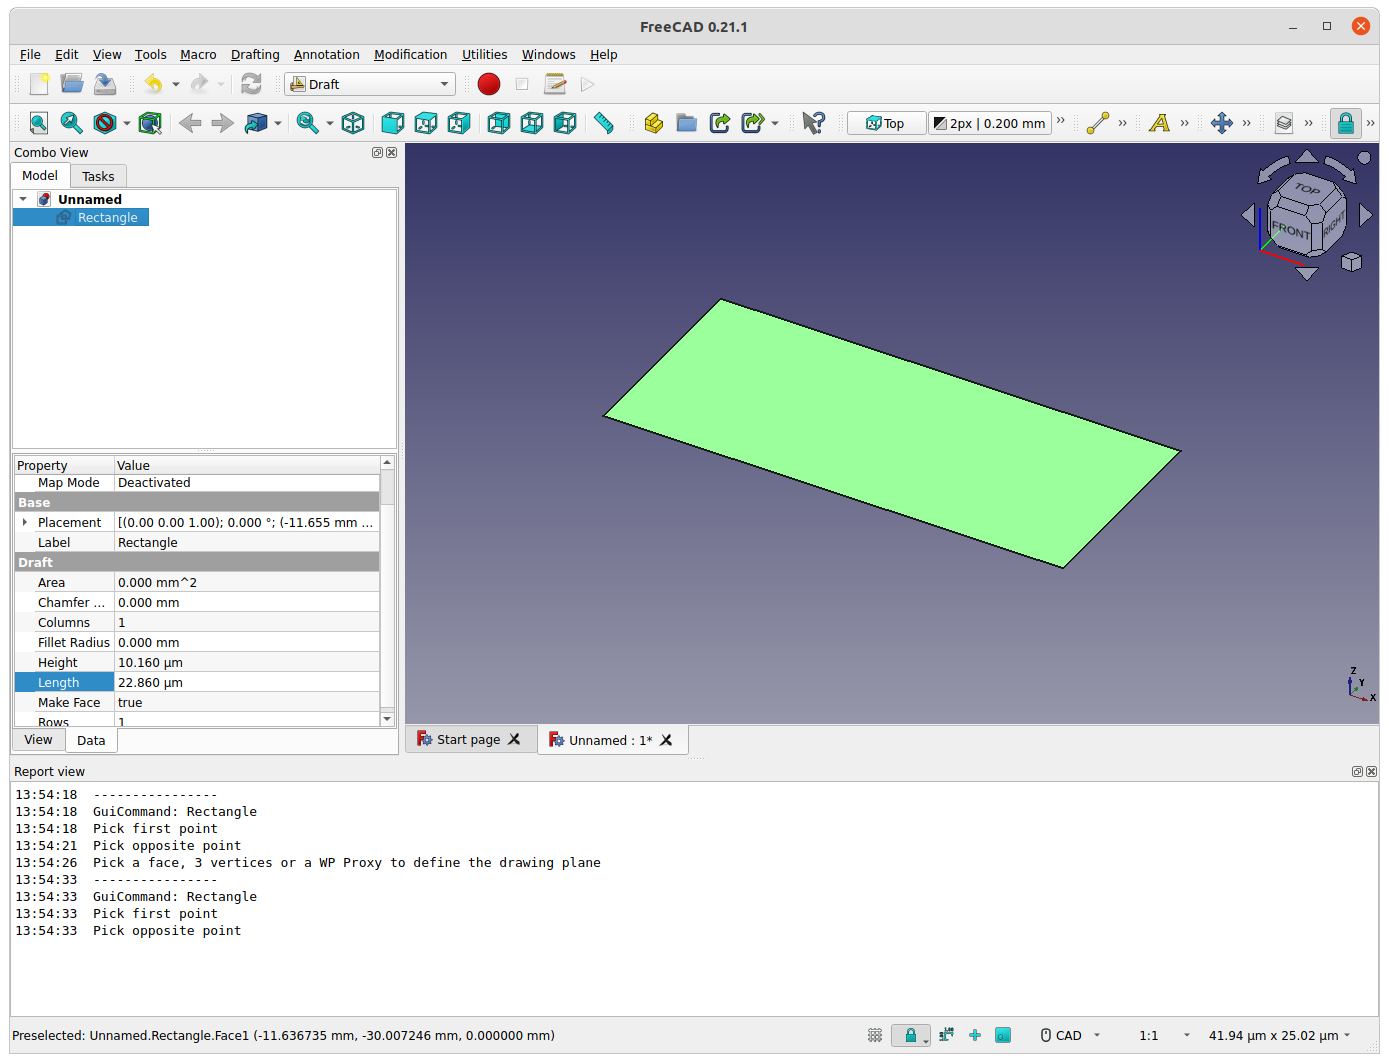
\includegraphics[width=0.75\textwidth]{../tutorials/OpenParEM3D/rectangular_waveguide/screenshots/rectangle}
  \caption{Screen shot of a rectangle sized for WR90 waveguide using $\mu$m for ultimate mm scaling.}
  \label{fig:rectangle}
\end{figure}
\item Switch to the \texttt{Part} Workbench with \texttt{View}$\rightarrow$\texttt{Workbench}$\rightarrow$\texttt{Part}.
\item Select the rectangle then select \texttt{Part}$\rightarrow$\texttt{Extrude ...}, then enter 100~um in the \texttt{Along} box.  Click \texttt{Ok}.
\item Select the item \texttt{Extrude} and view the \texttt{Properties} window to see the extrusion length in the \texttt{Length Fwd} value box.  If the length of the extrusion needs to be changed, change it here by editing the value of \texttt{Length Fwd}.
\item For learning purposes, change the extrusion length for the rectangle to 90 um and zoom to fit all.  A reference screen shot is shown in Fig.~\ref{fig:extrusion}.
\begin{figure}
  \centering
  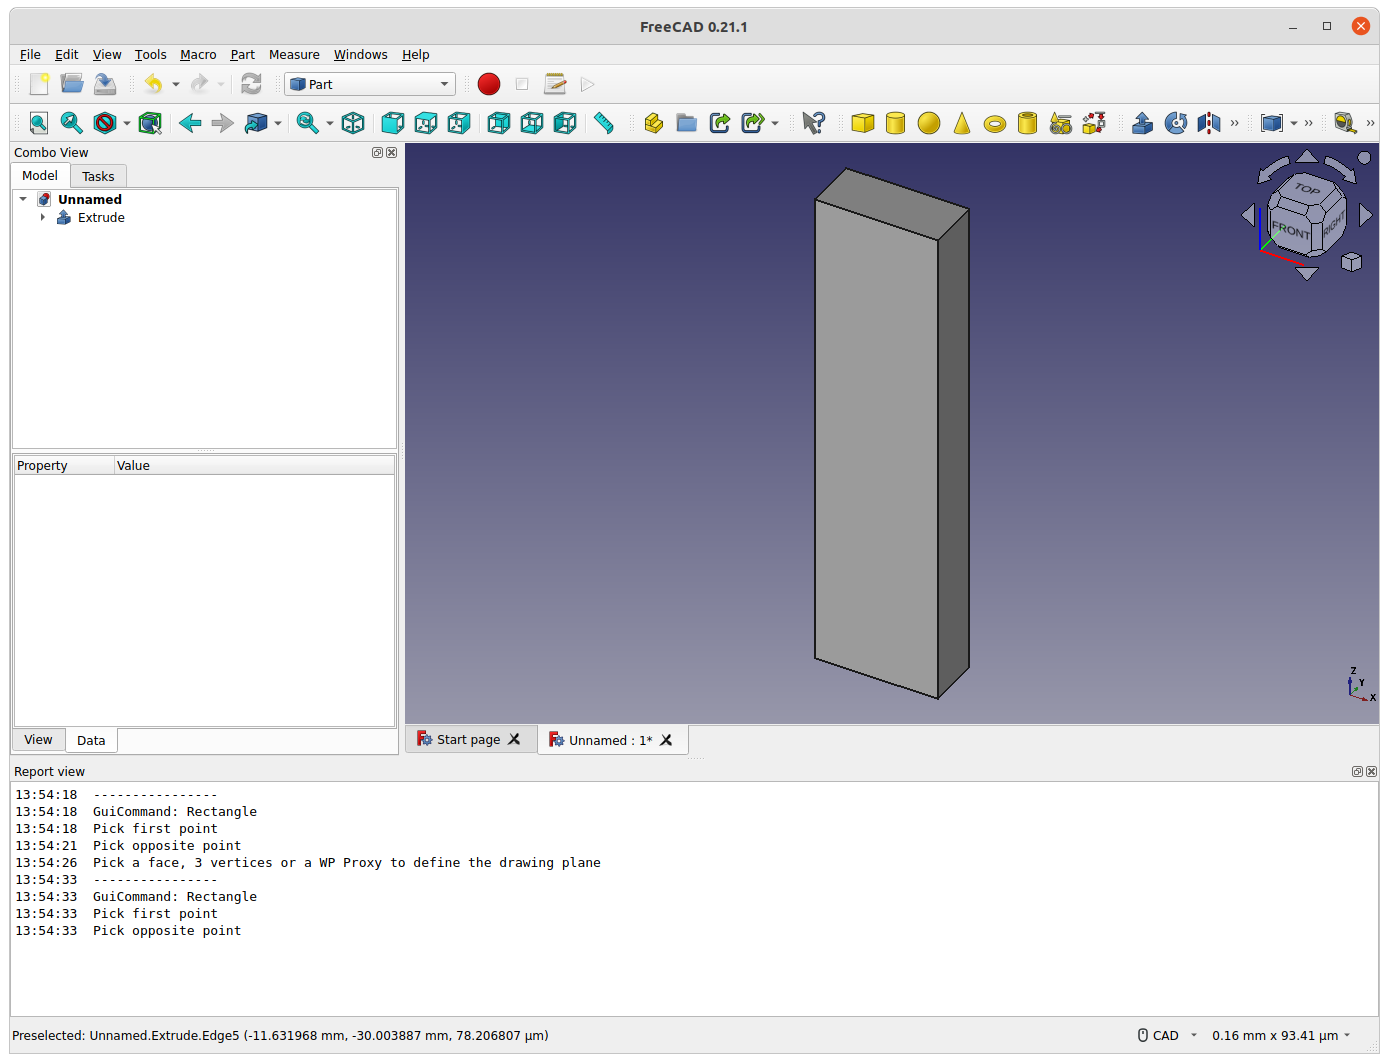
\includegraphics[width=0.75\textwidth]{../tutorials/OpenParEM3D/rectangular_waveguide/screenshots/extrusion}
  \caption{Screen shot of the rectangle extruded 90 um.}
  \label{fig:extrusion}
\end{figure}
\item In the \texttt{Combo View} window, click the small sideways triangle next to the \texttt{Extrude} item to show the \texttt{Rectangle} item.  Select the \texttt{Rectangle} item.  In the \texttt{Property} window, change the value of \texttt{Label} to \newline \texttt{\_Pportin}.  This rectangle marks the input port.
\item Change to the \texttt{Draft} workspace by selecting \texttt{View}$\rightarrow$\texttt{Workbench}$\rightarrow$\texttt{Draft}.
\item Save the drawing with the name \texttt{rectangular\_waveguide} using \texttt{File}$\rightarrow$\texttt{Save}.
\item Click on the end of the long extrusion that is opposite of \texttt{\_Pportin} then change the drawing plane to this plane by selecting \texttt{Utilities}$\rightarrow$\texttt{Select Plane}.  Alternatively, click the menu bar item as shown in Fig.~\ref{fig:portout} to change from \texttt{Top} to \texttt{Custom}.
\begin{figure}
  \centering
  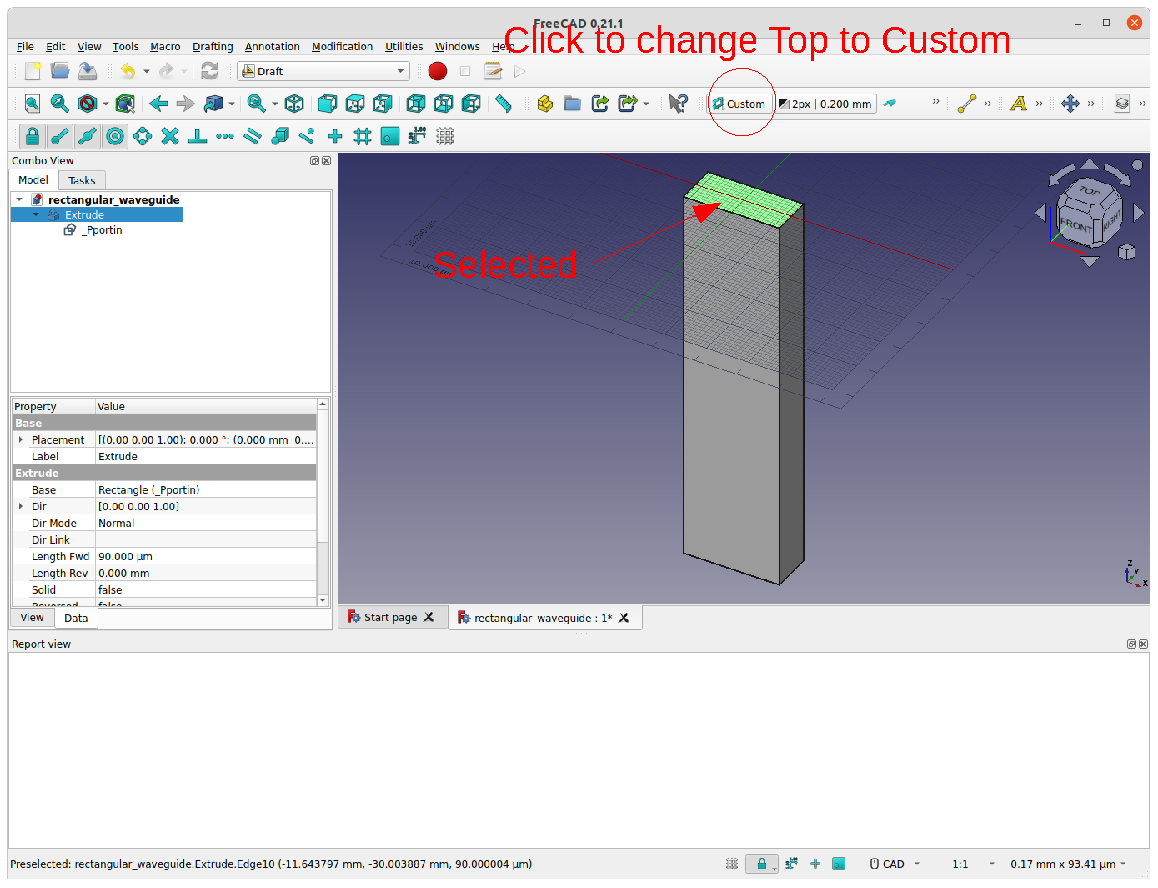
\includegraphics[width=0.75\textwidth]{../tutorials/OpenParEM3D/rectangular_waveguide/screenshots/portout-crop}
  \caption{Setting the drawing plane to the end of the extrusion.}
  \label{fig:portout}
\end{figure}
\item Draw a rectangle by snapping to diagonal corners of the end of the extrusion, then change the value of \texttt{Label} to \texttt{\_Pportout}. This rectangle marks the output port.
\item Hover the cursor over the \texttt{\_Pportout} in the \texttt{Combo View} window and the rectangle will highlight as shown in Fig.~\ref{fig:hover}.
\begin{figure}
  \centering
  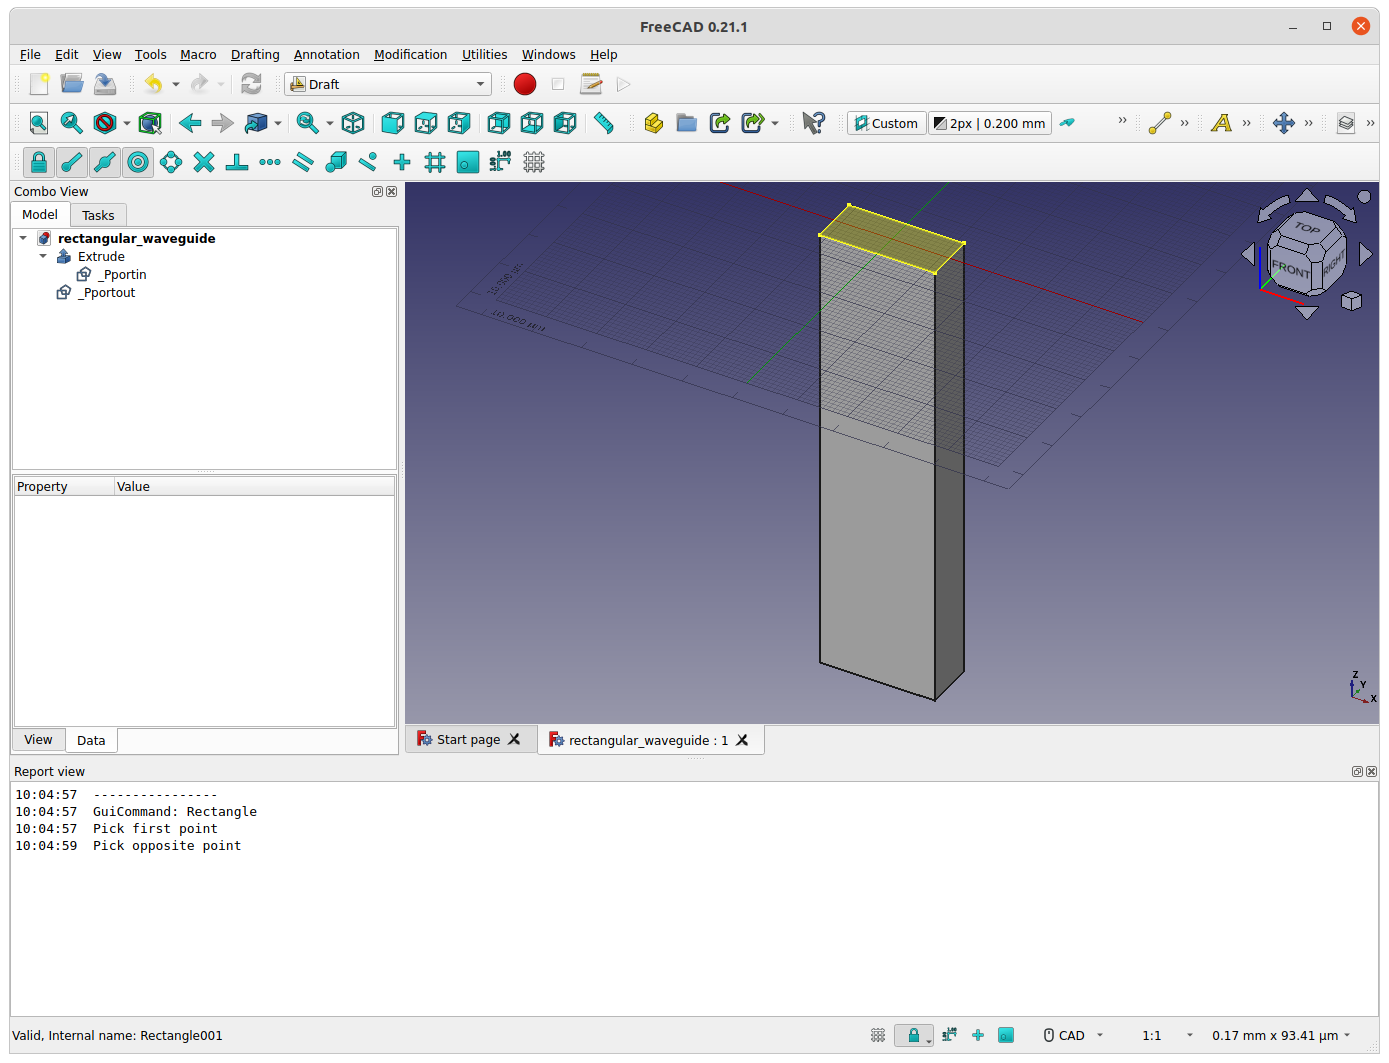
\includegraphics[width=0.75\textwidth]{../tutorials/OpenParEM3D/rectangular_waveguide/screenshots/hover}
  \caption{Hovering over the port object \hbox{\texttt{\_Pportout}} in the \texttt{Combo View} window highlights the output port.}
  \label{fig:hover}
\end{figure}
\item Expand the \texttt{lock} icon and select \texttt{Snap Midpoint}.  The screenshot in Fig.~\ref{fig:lock} shows the selection of the snapping to the midpoint of lines.
\begin{figure}
  \centering
  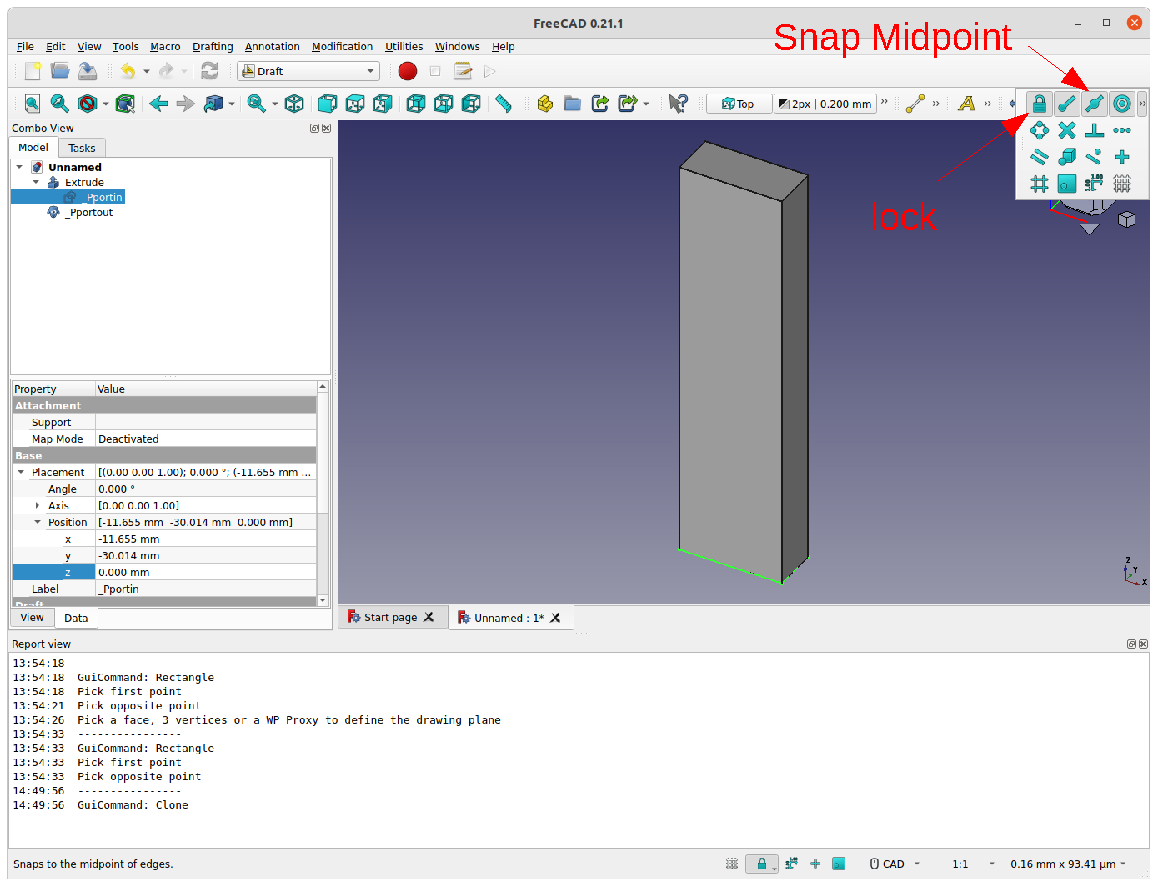
\includegraphics[width=0.75\textwidth]{../tutorials/OpenParEM3D/rectangular_waveguide/screenshots/lock-crop}
  \caption{Snapping selection showing snapping to line ends and centers and to face centers.}
  \label{fig:lock}
\end{figure}
\item View the input port with \texttt{View}$\rightarrow$\texttt{Standard views}$\rightarrow$\texttt{Bottom}.  Select line drawing with \texttt{Drafting}$\rightarrow$\texttt{Line} and draw a line from the center of the top of the rectangle to the bottom (i.e. directed in the $+$y direction).  Make sure it snaps to the line by only clicking when a white circle appears on the snap point.  It is critical that lines snap accurately to the geometry to avoid later errors in OpenParEM3D when things do not line up.  This line is the voltage integration line for the input port.  Change this line's \texttt{Label} to \texttt{\_Pvin}.
\item View the orthogonal view by selecting \texttt{View}$\rightarrow$\texttt{Standard views}$\rightarrow$\texttt{Home}. Draw a line from the bottom of the output port [long side] to the top of the port [long side] (i.e. directed in the $+$y direction).  Again, ensure that the line snaps to the middle of the side of the rectangle.  This line is the voltage integration line for the output port. Change this line's \texttt{Label} to \texttt{\_Pvout}.
\item Add a text item to the drawing by selecting \texttt{Annotation}$\rightarrow$\texttt{Text} and click anywhere in the drawing.  Enter a period in the popup text box, then click \texttt{Create text}. Select the new text object in the \texttt{Combo View} window, and change its \texttt{Label} to \texttt{\_Sin(PV)\{portin\}}.  This adds the input port using the power-voltage definition for characteristic impedance using the rectangle \texttt{\_Pportin}.
\item Repeat the adding of a text item, or copy/paste the existing one, and change its \texttt{Label} to \newline \texttt{\_Sout(PV)\{portout\}} to add the output port.
\item Add a text item and change its \texttt{Label} to \texttt{\_Min(1,voltage)\{vin\}} to add the S-parameter port 1 to port "in" using voltage calculation on the path defined by the line with label \texttt{\_Pvin}.
\item Add a text item and change its \texttt{Label} to \texttt{\_Mout(2,voltage)\{vout\}} to add the S-parameter port 2 to port "out" using voltage calculation on the path defined by the line with label \texttt{\_Pvout}.
\item Save the drawing since it is complete.
\item Select the \texttt{Extrude} object in the \texttt{Combo View} window, then export it with \texttt{File}$\rightarrow$\texttt{Export ...} then \texttt{Save}, removing the \verb+-Extrude+ part of the name.  The default format is \texttt{BREP} but can be verified before saving by checking the format drop-down.
\item Export the ports description file by selecting \texttt{Macro}$\rightarrow$\texttt{Macros ...}$\rightarrow$\texttt{OpenParEM3D\_save.py}$\rightarrow$\texttt{Execute}.  Enter the name \texttt{rectangular\_waveguide\_ports.txt}, then select \texttt{Save}.  Check the \texttt{Report view} window for errors.
\item A screen shot of the completed drawing with a successfully exported ports description file is shown in Fig.~\ref{fig:drawing_finished}.
\begin{figure}
  \centering
  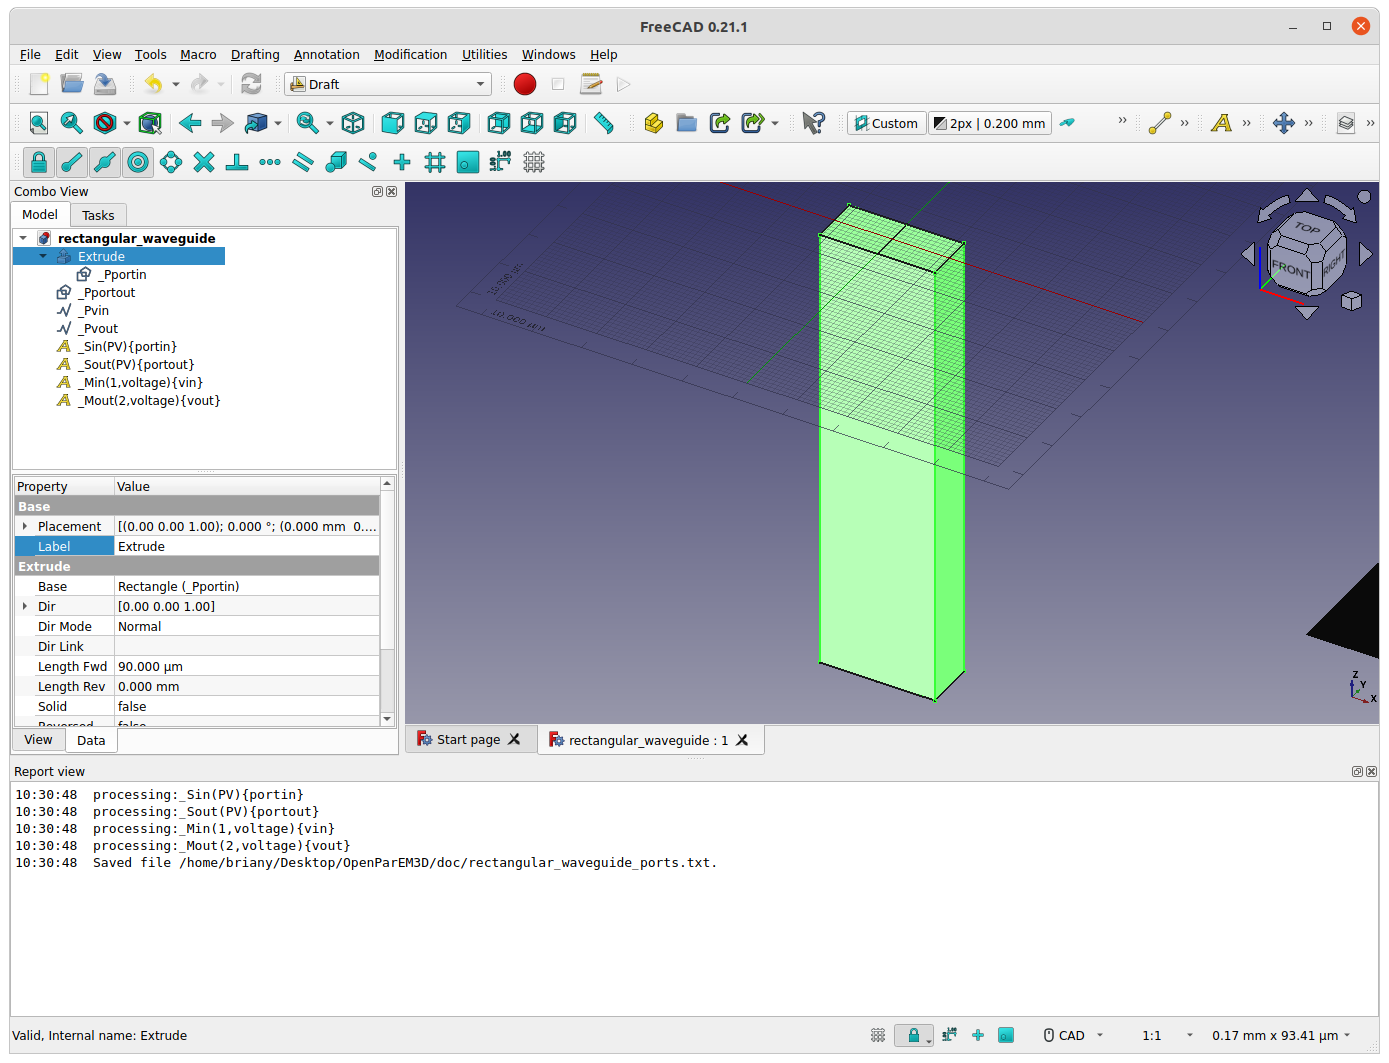
\includegraphics[width=0.75\textwidth]{../tutorials/OpenParEM3D/rectangular_waveguide/screenshots/drawing_finished}
  \caption{Screenshot of the completed drawing with exported ports description file.}
  \label{fig:drawing_finished}
\end{figure}
\item Save the drawing and exit FreeCAD.

\end{itemize}

\subsubsection{Meshing}

\begin{itemize}
\item Start gmsh as outlined in Sec.~\ref{sec:gmsh}.
\item Open the BREP file saved from the prior section by selecting \newline \texttt{File}$\rightarrow$\texttt{Open ...}$\rightarrow$\texttt{rectangular\_waveguide.brep}$\rightarrow$\texttt{Ok}.
\item Click and drag in the window to change the view.
\item Assign the material as air by clicking the options tree \newline$\boxplus$\texttt{Geometry}$\rightarrow$$\boxplus$\texttt{Physical Groups}$\rightarrow$$\boxplus$\texttt{Add}$\rightarrow$\texttt{Volume}.
\item In the pop-op window type \texttt{air} then select the yellow dot, which turns red.  Press the keyboard \texttt{e} and a new pop-up appears.  Click \texttt{Create new `.geo' file}.  Finally, press the keyboard \texttt{q} to finish.  [If the mouse does not select the dot, click the red box in the lower left to re-enable mouse input.]
\item To mesh the geometry, in the options tree click $\boxplus$\texttt{Mesh}$\rightarrow$\texttt{3D}. A screenshot of the mesh is shown in Fig.~\ref{fig:mesh}.
\begin{figure}
  \centering
  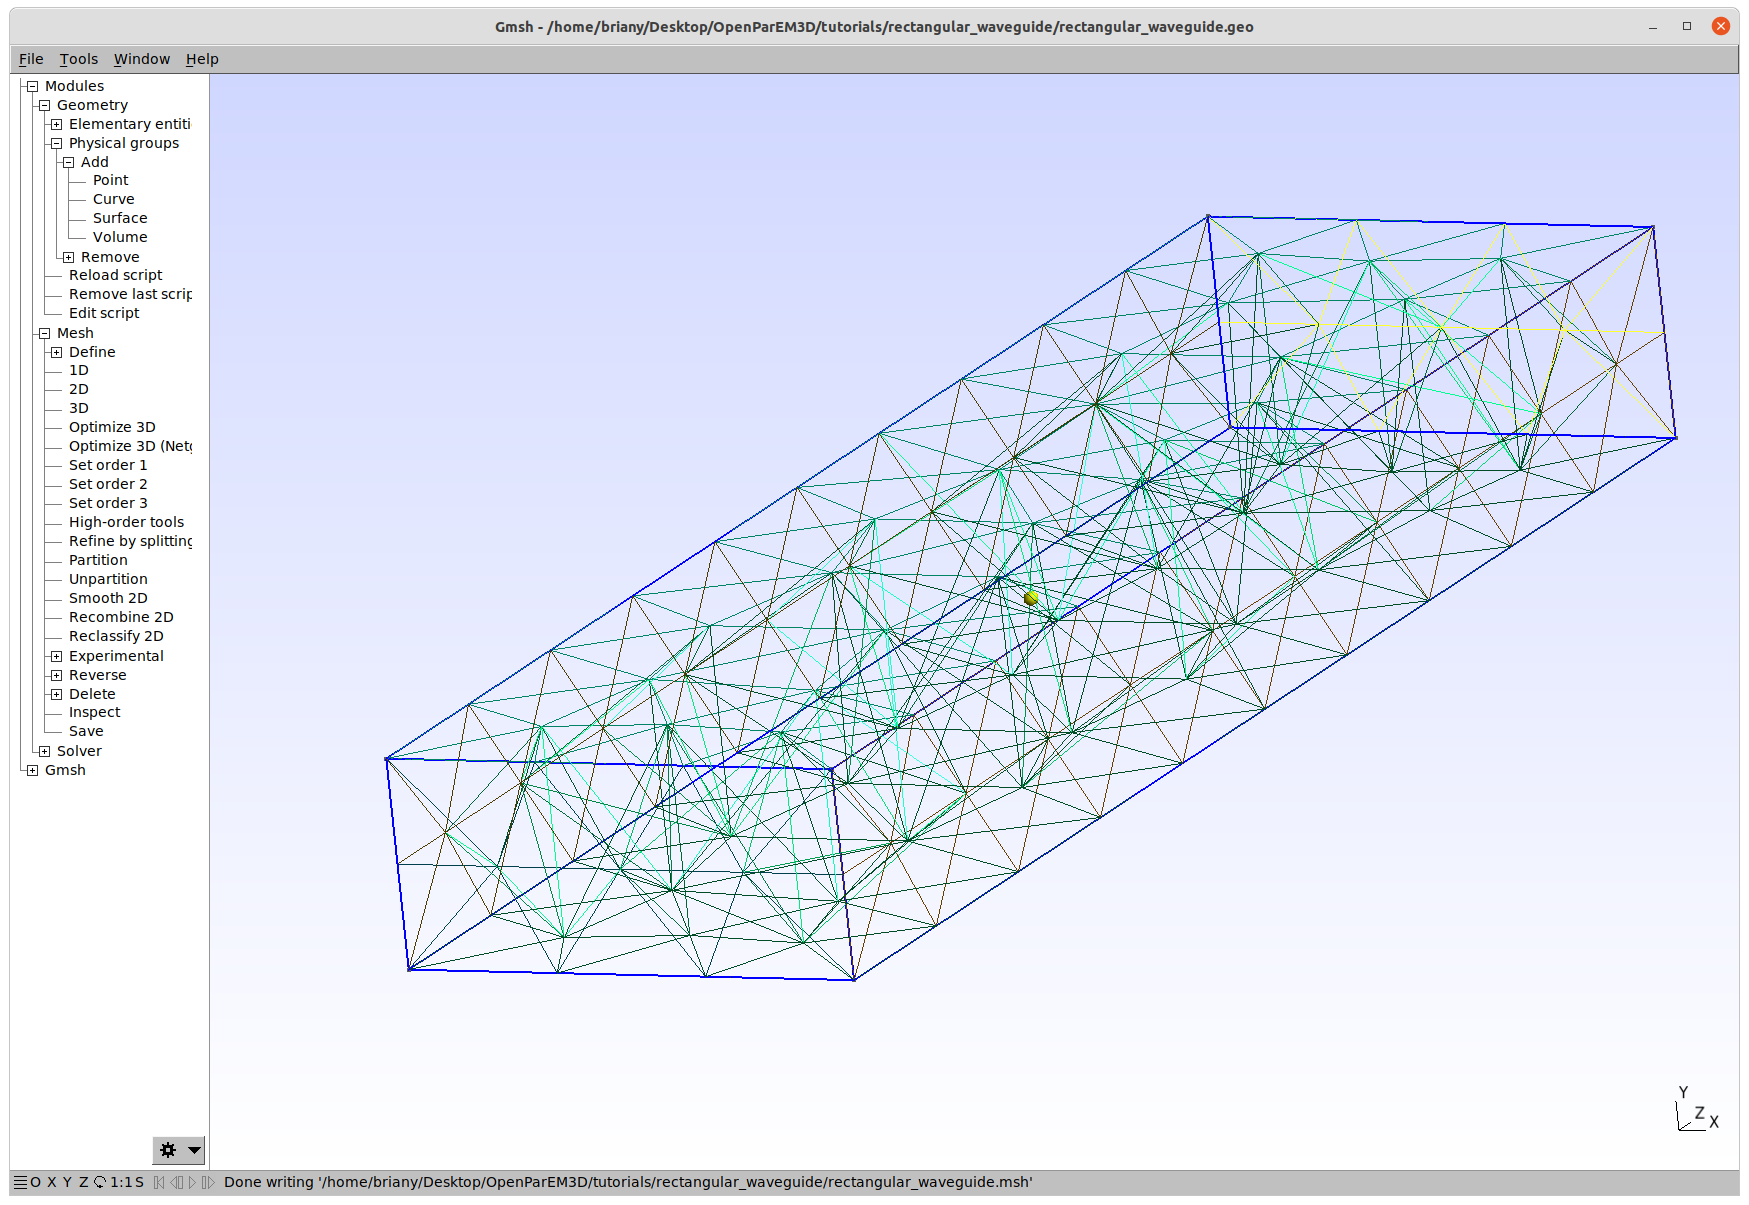
\includegraphics[width=0.75\textwidth]{../tutorials/OpenParEM3D/rectangular_waveguide/screenshots/mesh}
  \caption{Screenshot of the meshed straight section of rectangular waveguide.}
  \label{fig:mesh}
\end{figure}
\item Save the mesh by selecting \texttt{File}$\rightarrow$\texttt{Save Mesh}.
\item Quit gmsh.
\end{itemize}

\subsubsection{Solving}

\begin{itemize}

\item Create the materials file \texttt{global\_materials.txt} in any text editor and set the text contents to
\begin{Verbatim}[fontsize=\small]
  #OpenParEMmaterials 1.0
  Material
     name=air
     Temperature
        temperature=any
        Frequency
           frequency=any
           er=1.0006
           mur=1
           tand=0
           Rz=0
        EndFrequency
     EndTemperature
     Source
        Constantine A. Balanis, "Advanced Engineering Electromagnetics",
        John Wiley and Sons, 1989, p.79.
     EndSource
  EndMaterial
\end{Verbatim}
\item Create the project control file \texttt{rectangular\_waveguide.proj} in any text editor and set the text contents to
\begin{Verbatim}[fontsize=\small]
  #OpenParEM3Dproject 1.0
  project.save.fields            true
  mesh.file                      rectangular_waveguide.msh
  mesh.quality.limit             100
  mesh.order                     4
  port.definition.file           rectangular_waveguide_ports.txt
  materials.global.path          ./
  materials.global.name          global_materials.txt
  materials.local.path           ./
  materials.local.name           //local_materials.txt
  refinement.frequency           none
  refinement.iteration.min       1
  refinement.iteration.max       5
  refinement.required.passes     1
  refinement.relative.tolerance  1e-4
  refinement.variable            S
  frequency.plan.point           10e9
  reference.impedance            0
\end{Verbatim}

\noindent Note that iterative refinement is not needed for this problem since the mesh is fairly dense, 4$^{\textnormal{th}}$-order finite elements are used, and the fields vary slowly.  See Appendix~\ref{sec:control_file_spec} for a complete list of available keyword/value pairs that can be included in the project control file.

\item Run OpenParEM3D at the command line with
\begin{Verbatim}[fontsize=\small]
   $ OpenParEM3D rectangular_waveguide.proj
\end{Verbatim}
to run serially with a single core or with
\begin{Verbatim}[fontsize=\small]
   $ mpirun -q --oversubscribe -np 12 OpenParEM3D rectangular_waveguide.proj
\end{Verbatim}
to run in parallel with 12 cores.  Substitute a larger or smaller core number as needed.  The option \verb+--oversubscribe+ is not needed if the number of cores is less than or equal to half the number of available cores.
\item View the 2-port S-parameters, such as with \texttt{\$ more rectangular\_waveguide.s2p}, with the results looking very similar to 
\begin{Verbatim}[fontsize=\tiny]
! 2-port S-parameter data
! Sport 1 net1
! Sport 2 net2
# GHz S DB R 0
!freq dBS11 angS11 dBS21 angS21 dBS12 angS12 dBS22 angS22
10 -78.3715096672794 -55.5217603830515 0.000533264064487618 -96.4088426326485 0.000533264064487618 -96.4088426326485 -78.3907308077556 -52.6413868985043
\end{Verbatim}
These are serial results, and running in serial should produce almost identical results.  If running in parallel, due to the nature of MPI processing and iterative solution, the results can vary slightly.

Note the very high return loss since this is just a straight section of waveguide and the very slight positive insertion loss of 0.00053 dB since there are no conductor or dielectric losses.

From the result of the 2D simulations scrolled in the output when running OpenParEM3D, $\beta$=158.32151 rad/m.  Since the waveguide is 90~mm long, the expected phase shift is
 $\theta=-158.32151*0.090=-96.404^\circ$,
 which is in very close agreement to the 3D computed value of $-96.409^\circ$, or 0.0051\%.

\item Start ParaView at the command line with \verb+$ paraview &+, then navigate to and open the fields result \newline \texttt{rectangular\_waveguide\_frequency\_1e+10\_Sport\_1.pvd}
\item Click in the window and move the mouse to change the view.
\item Click on the box \texttt{Solid Color} then select \texttt{gridReE}.  Click \texttt{Apply} if nothing happens.
\item Click on the box \texttt{Magnitude} and select \texttt{Y} to view the y-component of the electric field.  A screen shot is shown in Fig.~\ref{fig:ReEy}.
\begin{figure}[H]
  \centering
  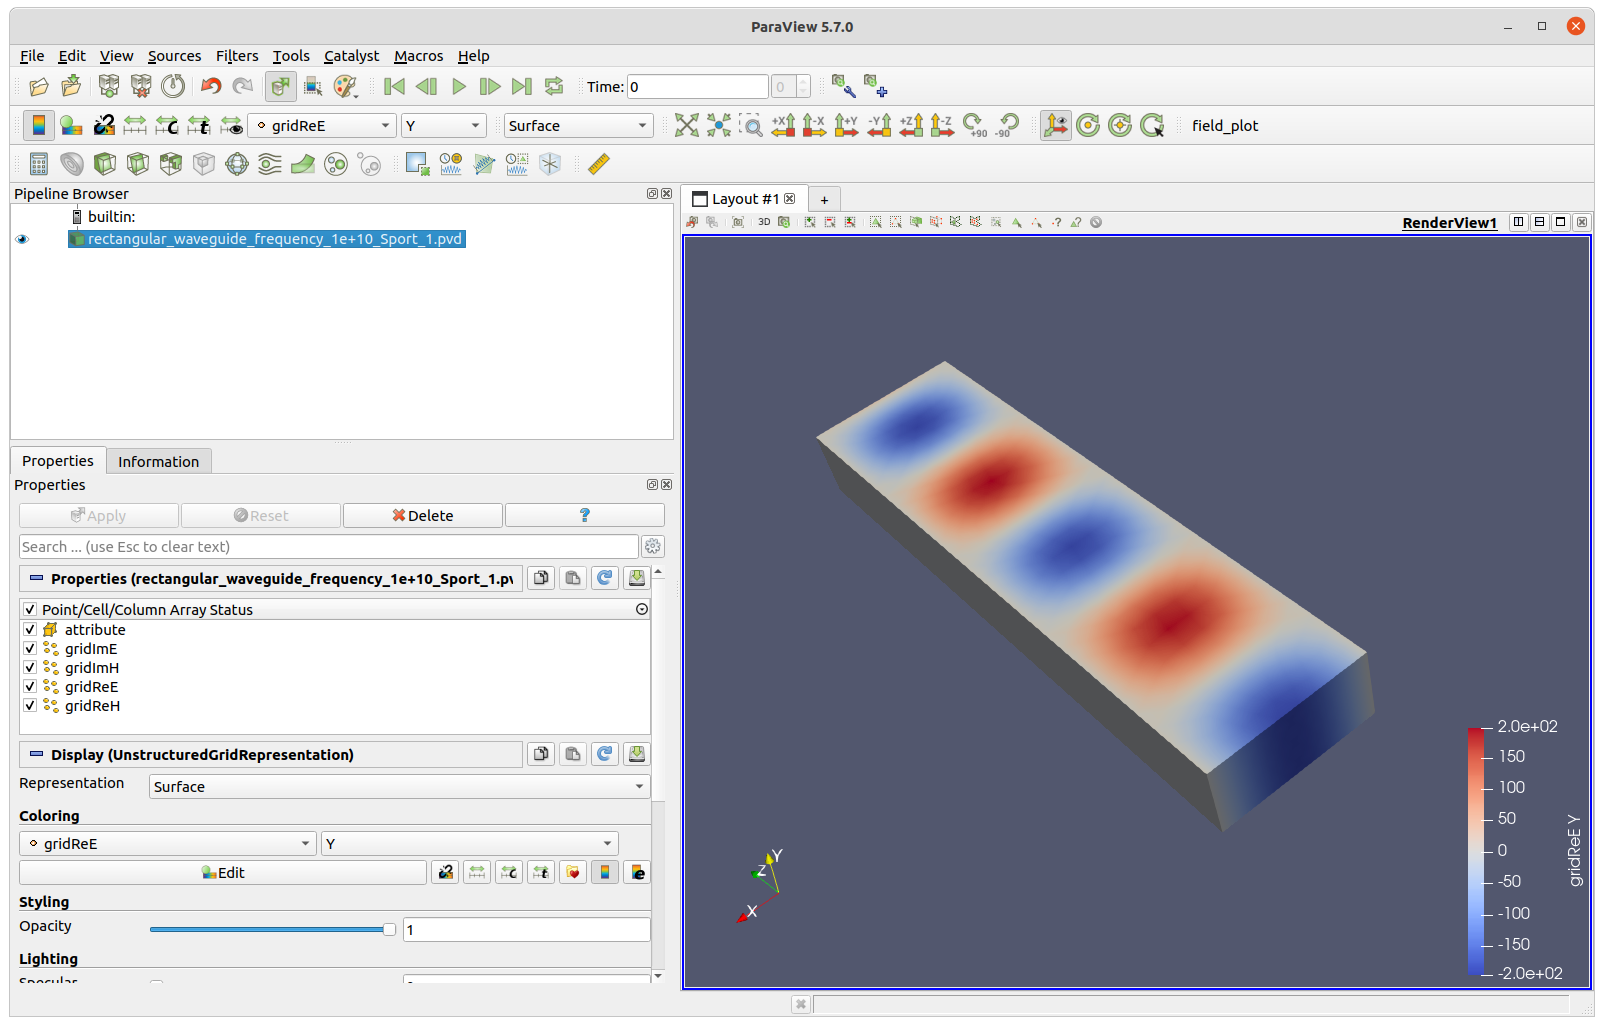
\includegraphics[width=0.75\textwidth]{../tutorials/OpenParEM3D/rectangular_waveguide/screenshots/ReEy}
  \caption{Re($E_y$) for the rectangular waveguide when driven by port 1.}
  \label{fig:ReEy}
\end{figure}
\item Vector plots can be viewed by selecting \texttt{Filters}$\rightarrow$\texttt{Alphabetical}$\rightarrow$\texttt{Glyph}.
\item Ensure that the \texttt{Glyph1} item in the \texttt{Pipeline Browser} is selected and that any other items are not.
\item Set \texttt{Orientation Array} to \texttt{gridReE} and the \texttt{Scale Array} to \texttt{gridReE}.
\item Set \texttt{Scale Factor} to 6.3e-05.
\item An outline of the geometry can be created by enabling \texttt{rectangular\_waveguide\_frequency\_1e+10\_Sport\_1.pvd}, then change \texttt{Representation} from \texttt{Surface} to \texttt{Outline}.
\item A similar plot for $\overline{H}$ can also be made.
\item Screenshots for $\overline{E}$ and $\overline{H}$ are shown in Fig.~\ref{fig:fields}.
\begin{figure}[H]
  \centering
  \begin{subfigure}{0.73\textwidth}
     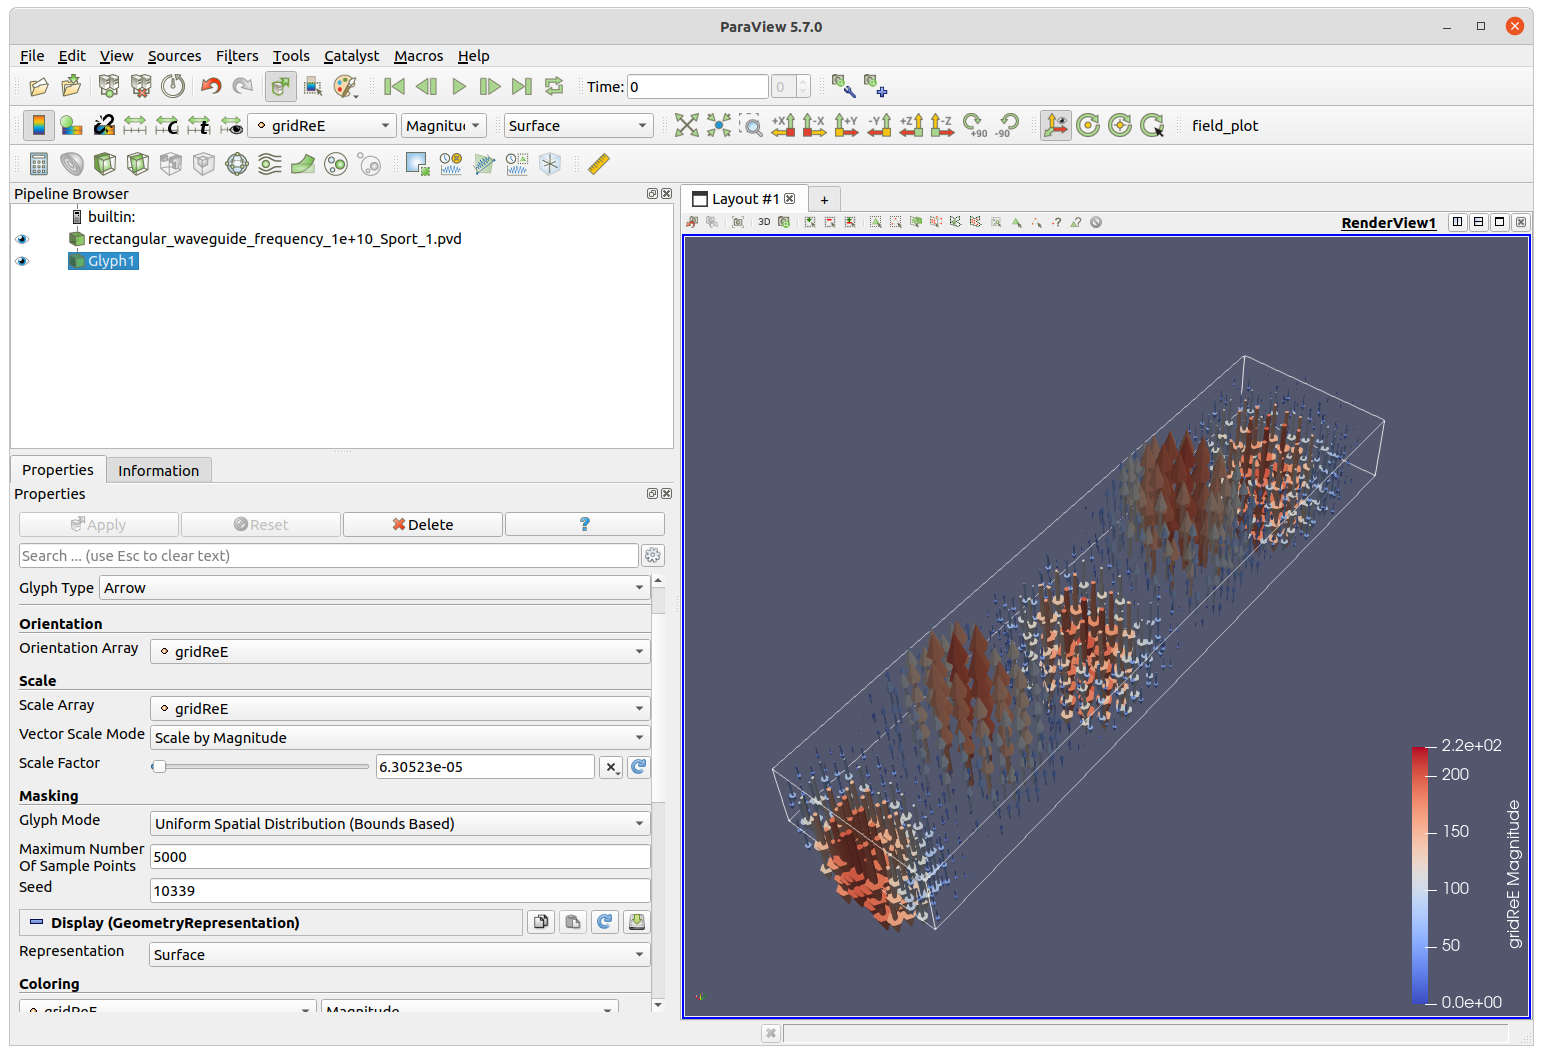
\includegraphics[width=\linewidth]{../tutorials/OpenParEM3D/rectangular_waveguide/screenshots/ReE} 
     \caption{Re($\overline{E}$)}
  \end{subfigure}
  \par\bigskip
  \begin{subfigure}{0.73\textwidth}
     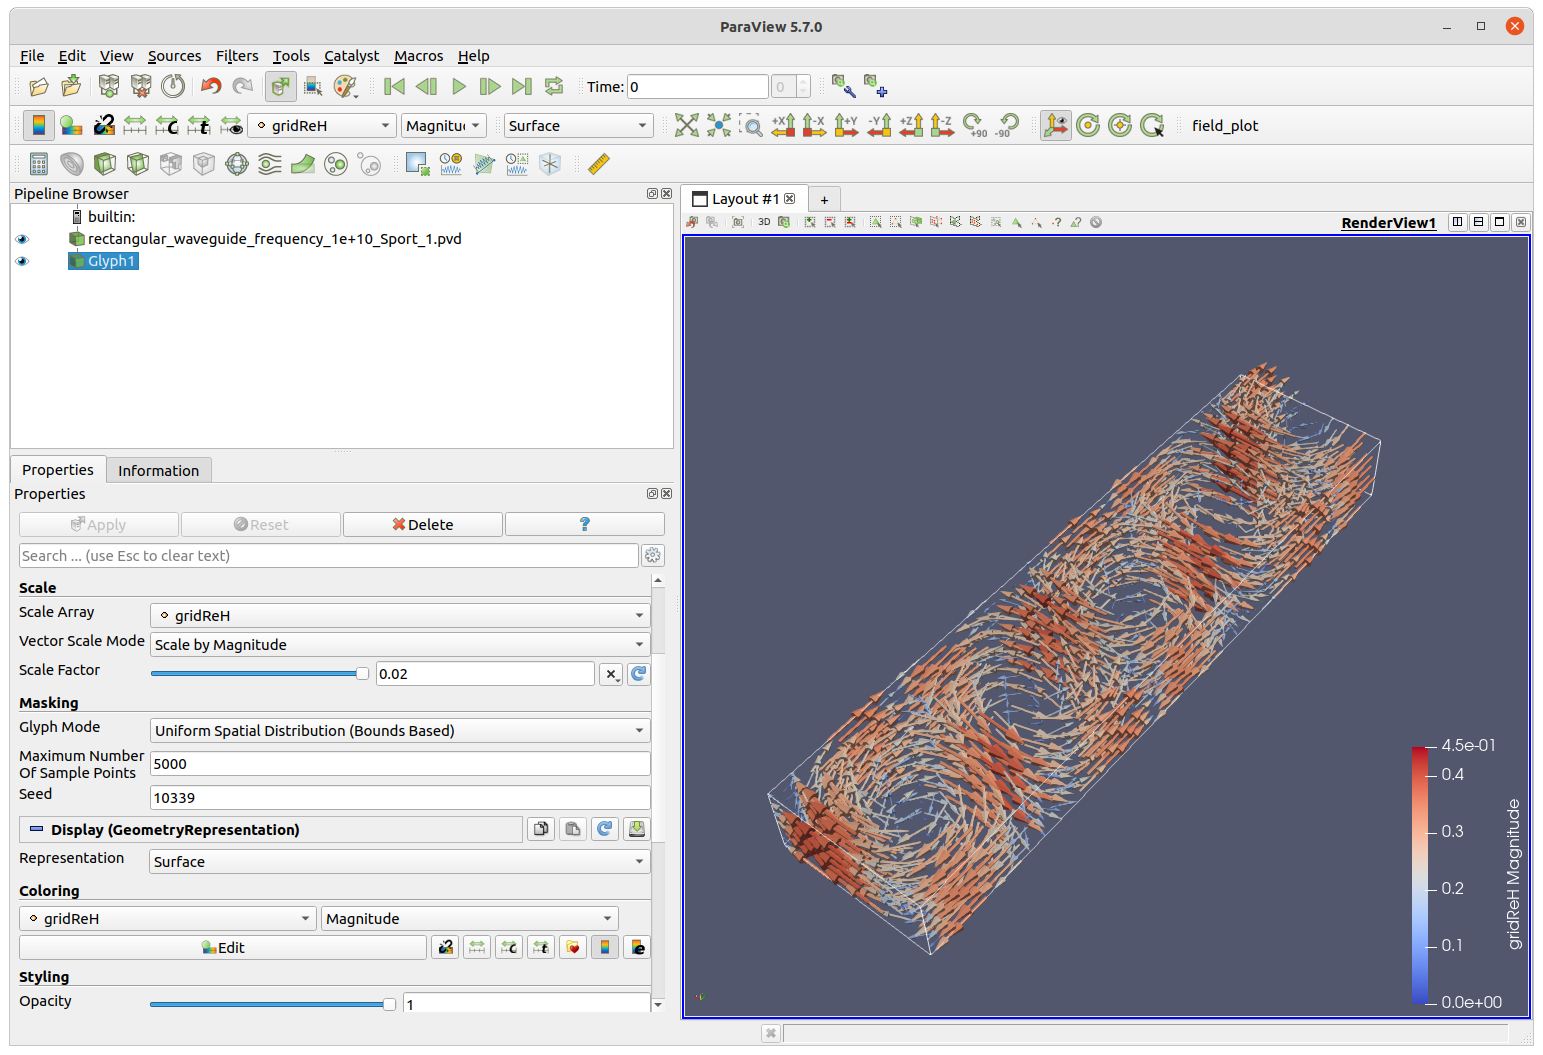
\includegraphics[width=\linewidth]{../tutorials/OpenParEM3D/rectangular_waveguide/screenshots/ReH}
     \caption{Re($\overline{H}$)}
  \end{subfigure}
  \caption{Vector fields for the rectangular waveguide when driven by port 1.}
  \label{fig:fields}
\end{figure}

\end{itemize}

\subsection{Microstrip Step in Width}

A straight section of microstrip with a step in width is constructed, annotated for 2-port S-parameter simulation, meshed, and solved.

\subsubsection{Drawing and Port Annotation}

\begin{itemize}
\item Create a directory for the project
\begin{Verbatim}[fontsize=\small]
$ mkdir microstrip_step
$ cd microstrip_step
\end{Verbatim}
\item Start FreeCAD, open a new drawing, set preferences [if needed], set the drawing workspace to \texttt{Draft}, and set the drawing plane to \texttt{Top} as outlined in Sec.~\ref{sec:freecad}.
\item Four rectangles are needed to eventually form the substrate, the input microstrip line, the output microstrip line, and the air above.  Add four rectangles and modify the properties to get them started.  Continuing the work-around with FreeCAD, the drawing is done in $\mu$m to end up with a mesh in mm.
\begin{itemize}
  \item Substrate: \texttt{label}$\rightarrow$\texttt{substrate2D}; \texttt{height}$\rightarrow$\texttt{0.254um}; \texttt{length}$\rightarrow$\texttt{2.54um}
  \item Input Microstrip: \texttt{label}$\rightarrow$\texttt{input2D}; \texttt{height}$\rightarrow$\texttt{0.025um}; \texttt{length}$\rightarrow$\texttt{0.254um}
  \item Output Microstrip: \texttt{label}$\rightarrow$\texttt{output2D}; \texttt{height}$\rightarrow$\texttt{0.025um}; \texttt{length}$\rightarrow$\texttt{0.508um}
  \item Air: \texttt{label}$\rightarrow$\texttt{air2D}; \texttt{height}$\rightarrow$\texttt{1.27um}; \texttt{length}$\rightarrow$\texttt{2.54um}
\end{itemize}
\item Position \texttt{substrate2D} to the origin by changing the properties \texttt{Base}$\rightarrow$\texttt{Placement}$\rightarrow$\texttt{Position}$\rightarrow$\texttt{x} to 0 and similarly for \texttt{y} and \texttt{z}.
\item Enable snapping to center as shown in Fig.~\ref{fig:lock}.
\item Select the object \texttt{air2D} then move it to snap the center of the bottom to the center of the top of the object \texttt{substrate2D} using \texttt{Modification}$\rightarrow$\texttt{Move}.  To do this, bring the mouse near the desired snap location until the white dot appears to show that the snap point is active, click and release the mouse, drag to the desired location until another white dot appears, then click to complete the move.  It is critical to click for the moves only with the white dots showing to achieve proper alignment.
\item Similar to \texttt{air2D}, select the object \texttt{input2D} and move/snap the bottom center to the top center of \texttt{substrate2D}.  Repeat for \texttt{output2D}.
\item If an object is in the way and prevents picking up the snap points of another object, hide the object by selecting it and pressing the space bar.  Unhide by selecting it in the \texttt{Combo View} window and pressing the space bar.
\item The project should look like the screen shot in Fig.~\ref{fig:microstrip2D}.
\begin{figure}
  \centering
  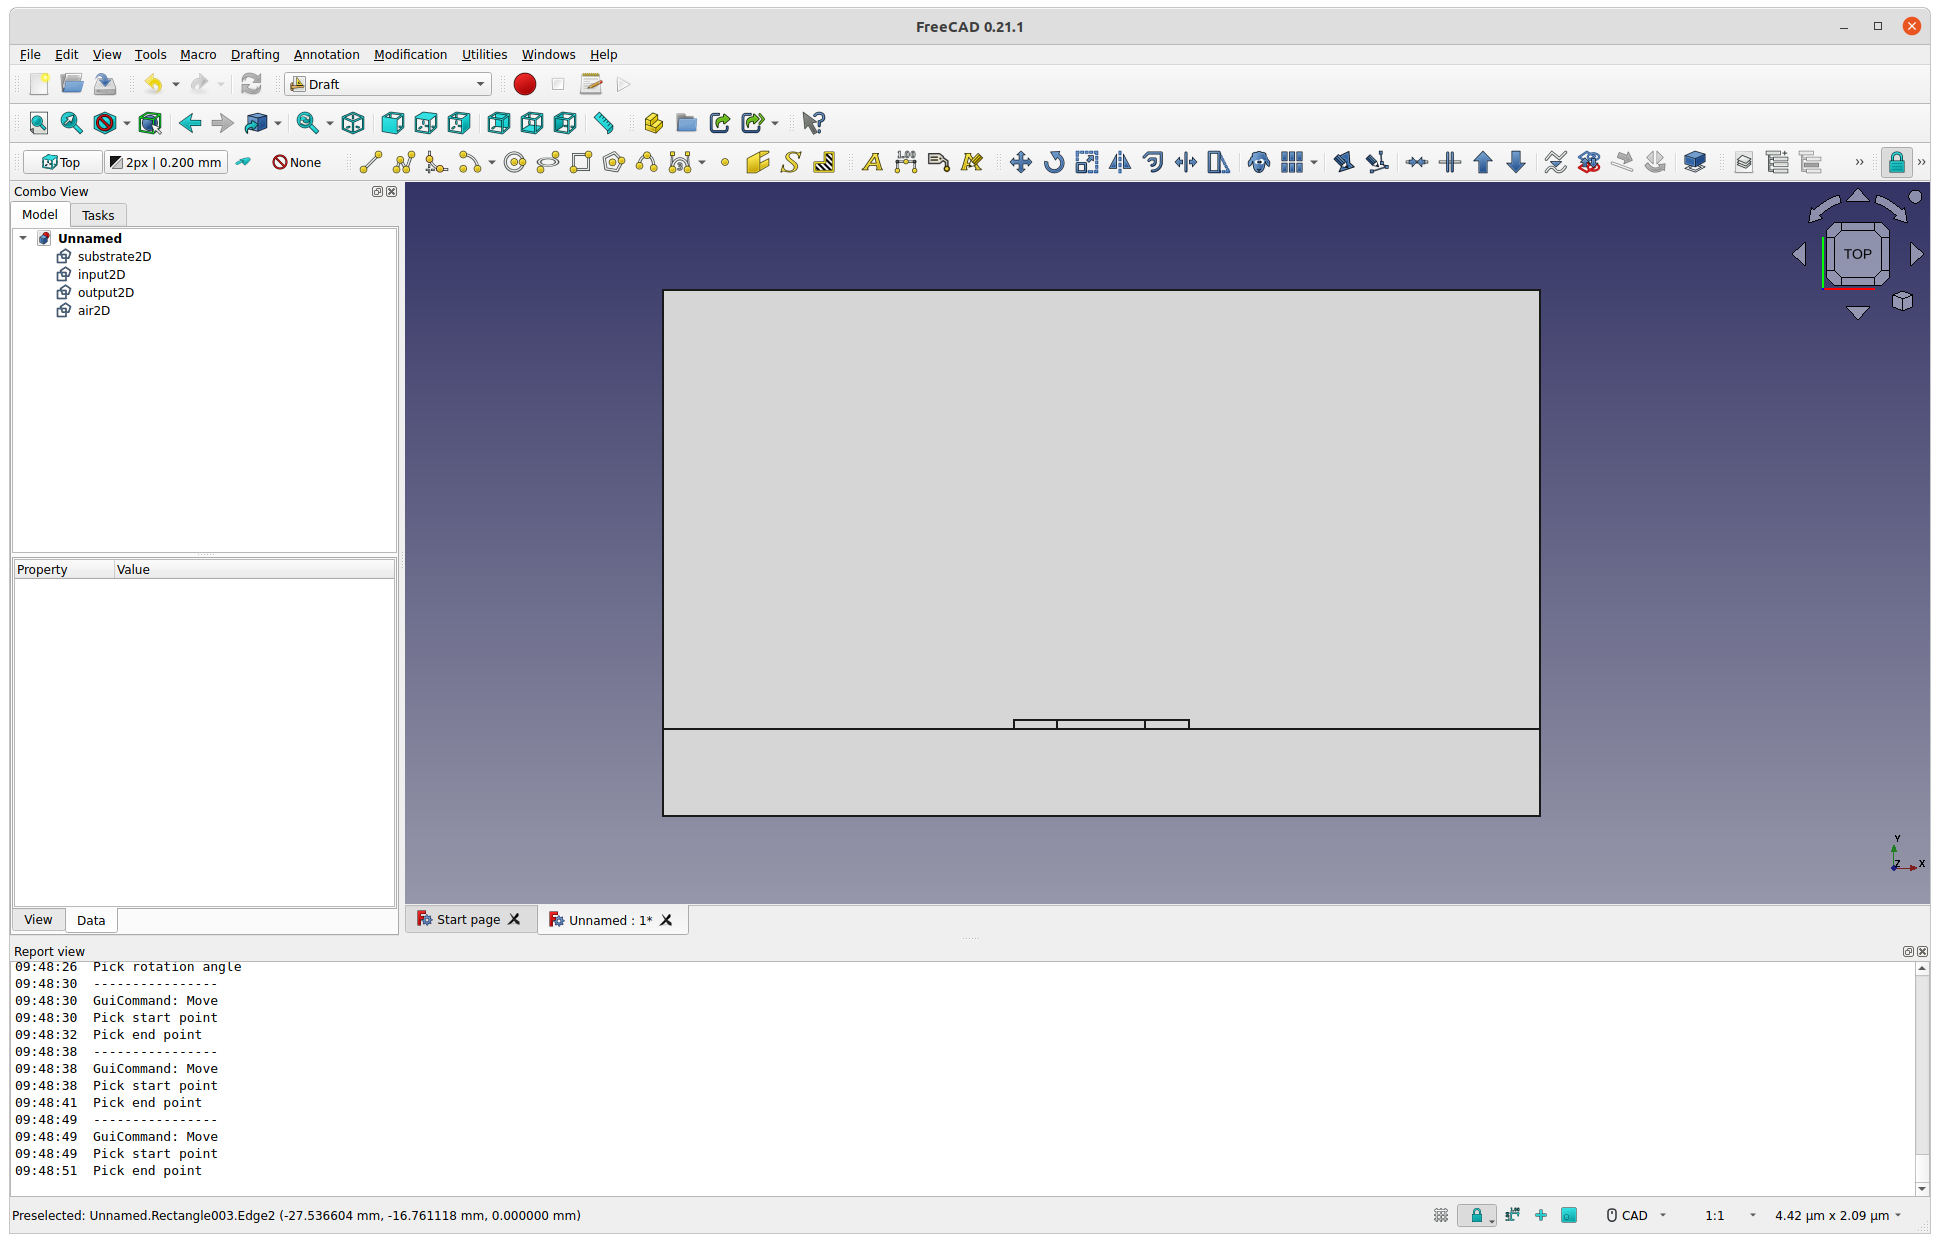
\includegraphics[width=0.75\textwidth]{../tutorials/OpenParEM3D/microstrip_step/screenshots/microstrip2D}
  \caption{Screenshot of the 2D setup for the microstrip-step-in-width tutorial.}
  \label{fig:microstrip2D}
\end{figure}
\item Save the drawing as \texttt{microstrip\_step}.
\item Change the workspace from \texttt{Draft} to \texttt{Part}.
\item Select all four rectangles, then \texttt{Part}$\rightarrow$\texttt{Extrude ...}$\rightarrow$\texttt{Along} and enter \texttt{10um} to extrude each box 10~$\mu$m.
\item Change the label of each extrusion to match the label of the underlying rectangle, so for example, \texttt{Extrude} is changed to \texttt{substrate}.
\item Put the display in a convenient view by \texttt{View}$\rightarrow$\texttt{Standard Views}$\rightarrow$\texttt{Home}.
\item Select the object \texttt{substrate} and hide it by pressing the space bar.
\item Select \texttt{input} and change the property \texttt{Length fwd} to \texttt{5um} to make it half as long.  Repeat for \texttt{output}.
\item Change back to the \texttt{Draft} workspace, then select \texttt{output} and move it 5~$\mu$m so that the near end snaps to the far end of \texttt{input}.  The two microstrip lines should be co-linear and end-to-end, as shown in Fig.~\ref{fig:microstrip_extrusion}.
\begin{figure}
  \centering
  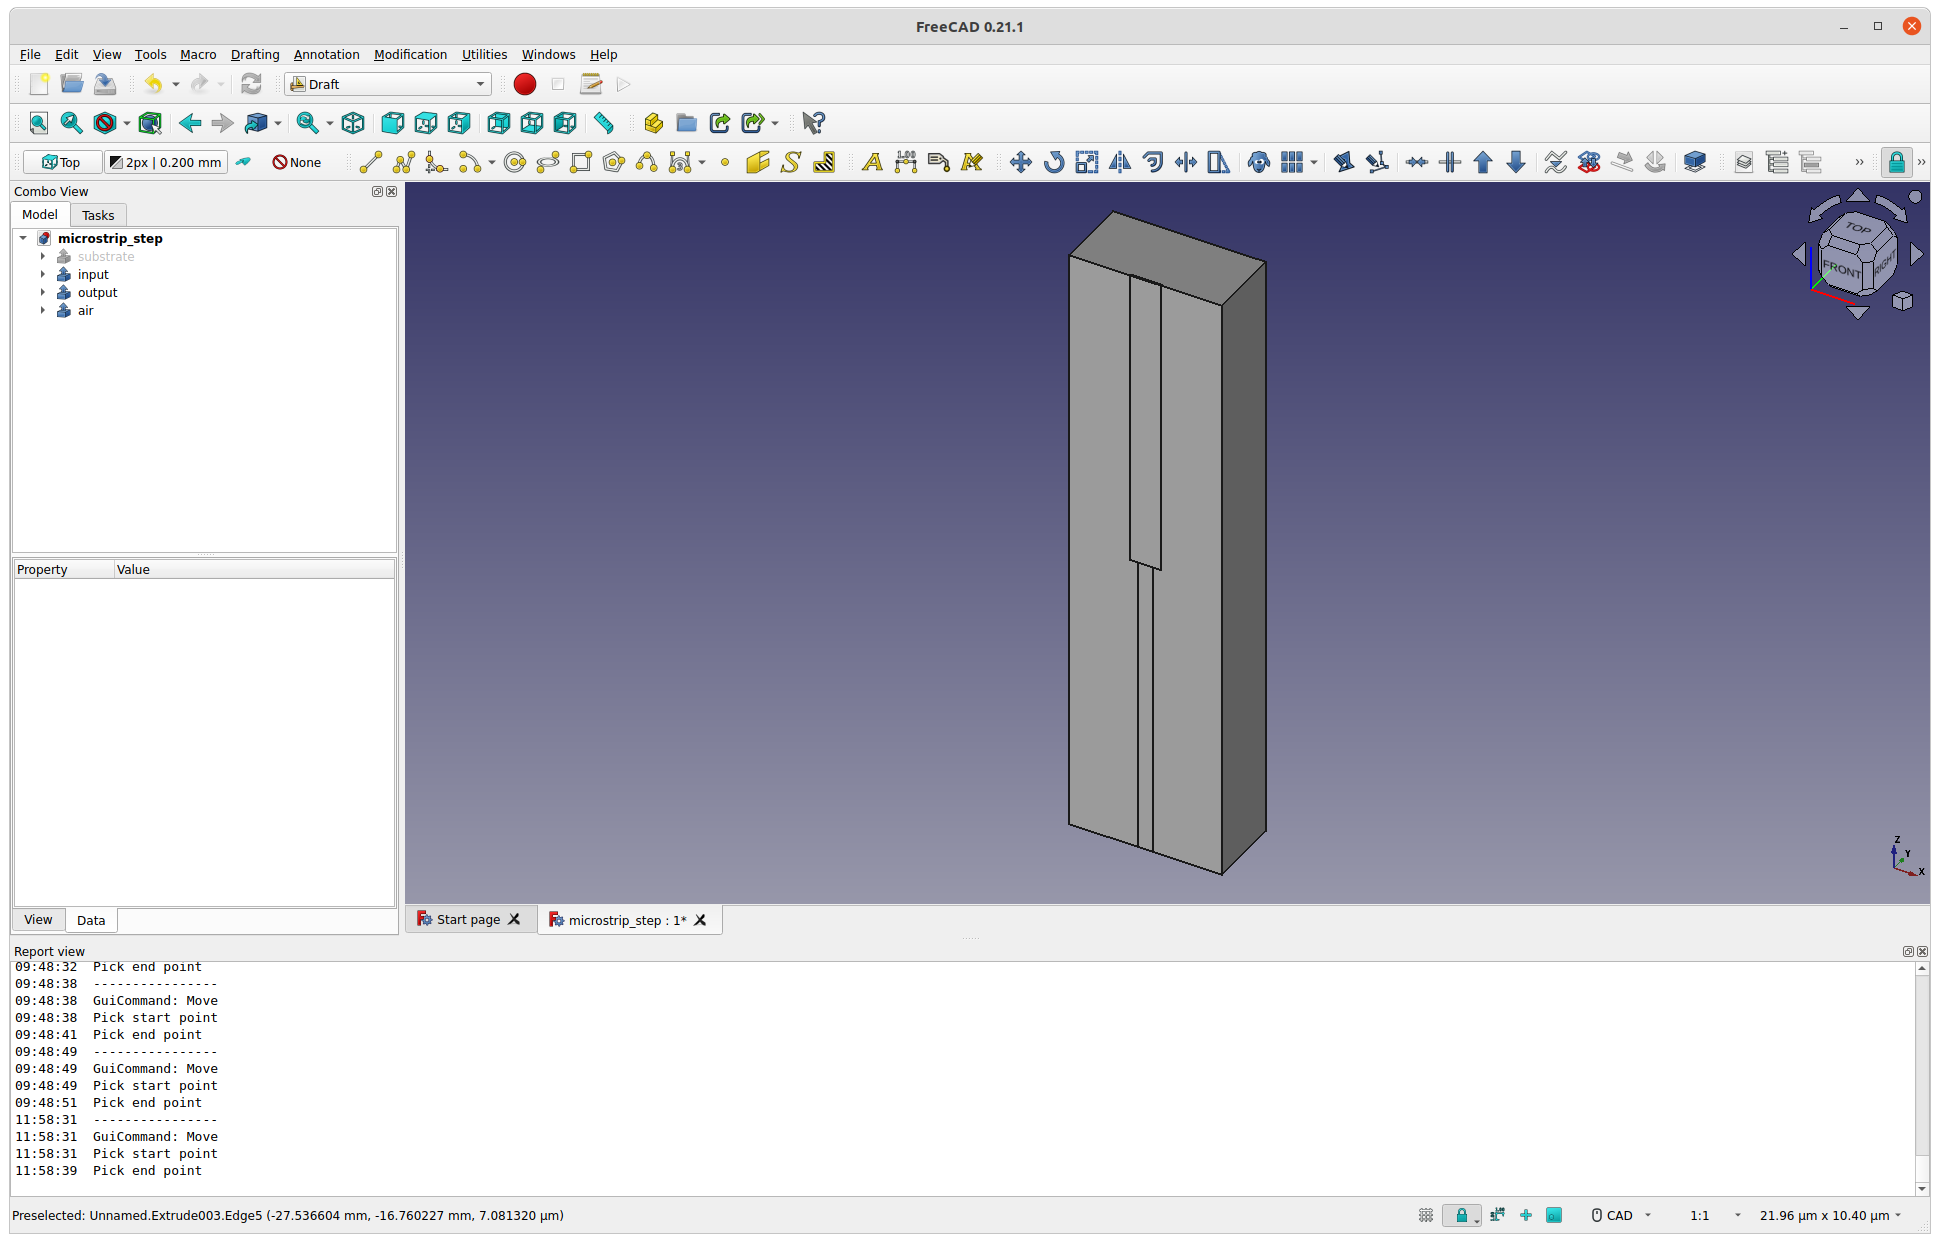
\includegraphics[width=0.75\textwidth]{../tutorials/OpenParEM3D/microstrip_step/screenshots/microstrip_extruded}
  \caption{Screenshot of the 3D setup after extrusion and movement of one microstrip segment.}
  \label{fig:microstrip_extrusion}
\end{figure}
\item All surfaces \textit{outside} the drawn geometry default to perfect electric conductors, so metal.  \textit{Outside} means a void where there is no geometry defined.  To create the microstrip lines, the drawn microstrips can be Boolean subtracted from the air to create the needed voids.  To do this, switch back to the \texttt{Part} workspace, select \texttt{air}, then add \texttt{input} to the selection by selecting it with the \texttt{Ctrl} key pressed, then select \texttt{Part}$\rightarrow$\texttt{Boolean}$\rightarrow$\texttt{Cut}.  Select the newly created cut item then add \texttt{output} to the selection and repeat the cut operation.  Change the label of the final cut object to \texttt{air\_metal}.
\item Select \texttt{substrate} and press the spacebar to enable viewing it.
\item Select \texttt{air\_metal} and \texttt{substrate}, then merge them by selecting \texttt{Part}$\rightarrow$\texttt{Split}$\rightarrow$\texttt{Boolean fragments}. 
\item Select the Boolean fragments object then export it a BREP file with the name \texttt{microstrip\_step.brep}.
\item At this point, there is a 3D substrate and 3D air with a void where the microstrip metal exists.  It is ready for port annotation.
\item Set up the port at the top for adding annotations by setting the workspace to \texttt{Draft}, selecting \texttt{View}$\rightarrow$\texttt{Standard views}$\rightarrow$\texttt{Top}, clicking on one of the rectangle faces to select it, and selecting the plane as the drawing plane with \texttt{Utilities}$\rightarrow$\texttt{Select Plane} or by clicking the related tool bar button.
\item To form the output port outline, draw a rectangle covering the full cross section and change the label to \texttt{\_Pportout}.
\item To add the output port current integration path, draw a rectangle over the microstrip and change the label to \texttt{\_PIout}.
\item To add the output port voltage integration path, draw a line from the center of the bottom of the substrate to the center of the microstrip line at the interface to the substrate and change the label to \texttt{\_PVout}.  Ensure that snapping-to-center is on for this operation.
\item For the input port, selecting \texttt{View}$\rightarrow$\texttt{Standard views}$\rightarrow${Bottom}, select a rectangle face, and set the drawing plane.  Add rectangles for \texttt{\_Pportin} and \texttt{\_PIin} and a line for \texttt{\_PVin}.  Note that the directions of the voltage lines between the two ports must be the same to avoid an extra $180^\circ$ phase shift, so both need to go from the ground to the strip or from the strip to the ground.  If the strip-to-ground direction is drawn, then the characteristic impedance using the V/I definition will be negative [which does not hurt anything].
\item Add text objects with labels to complete the ports with labels \texttt{\_Sin(PV){portin}}, \texttt{\_Min(1,voltage){Vin}}, \texttt{\_Min(1,current){Iin}}, \texttt{\_Sin(PV){portout}}, \texttt{\_Mout(2,voltage){Vout}}, and \texttt{\_Mout(2,current){Iout}}.  Since the PV definition for characteristic impedance is called out, the current mode definitions are not used.  The input microstrip port is S-parameter port 1, while the output microstrip port is S-parameter port 2.
\item Export the ports description file by selecting \texttt{Macro}$\rightarrow$\texttt{Macros ...}$\rightarrow$\texttt{OpenParEM3D\_save.py}$\rightarrow$\texttt{Execute}.  Enter the name \texttt{microstrip\_step\_ports.txt}, then select \texttt{Save}.  Check the \texttt{Report view} window for errors.
\item A screen shot of the completed drawing with successfully export ports description file is shown in Fig.~\ref{fig:microstrip3D}.
\begin{figure}
  \centering
  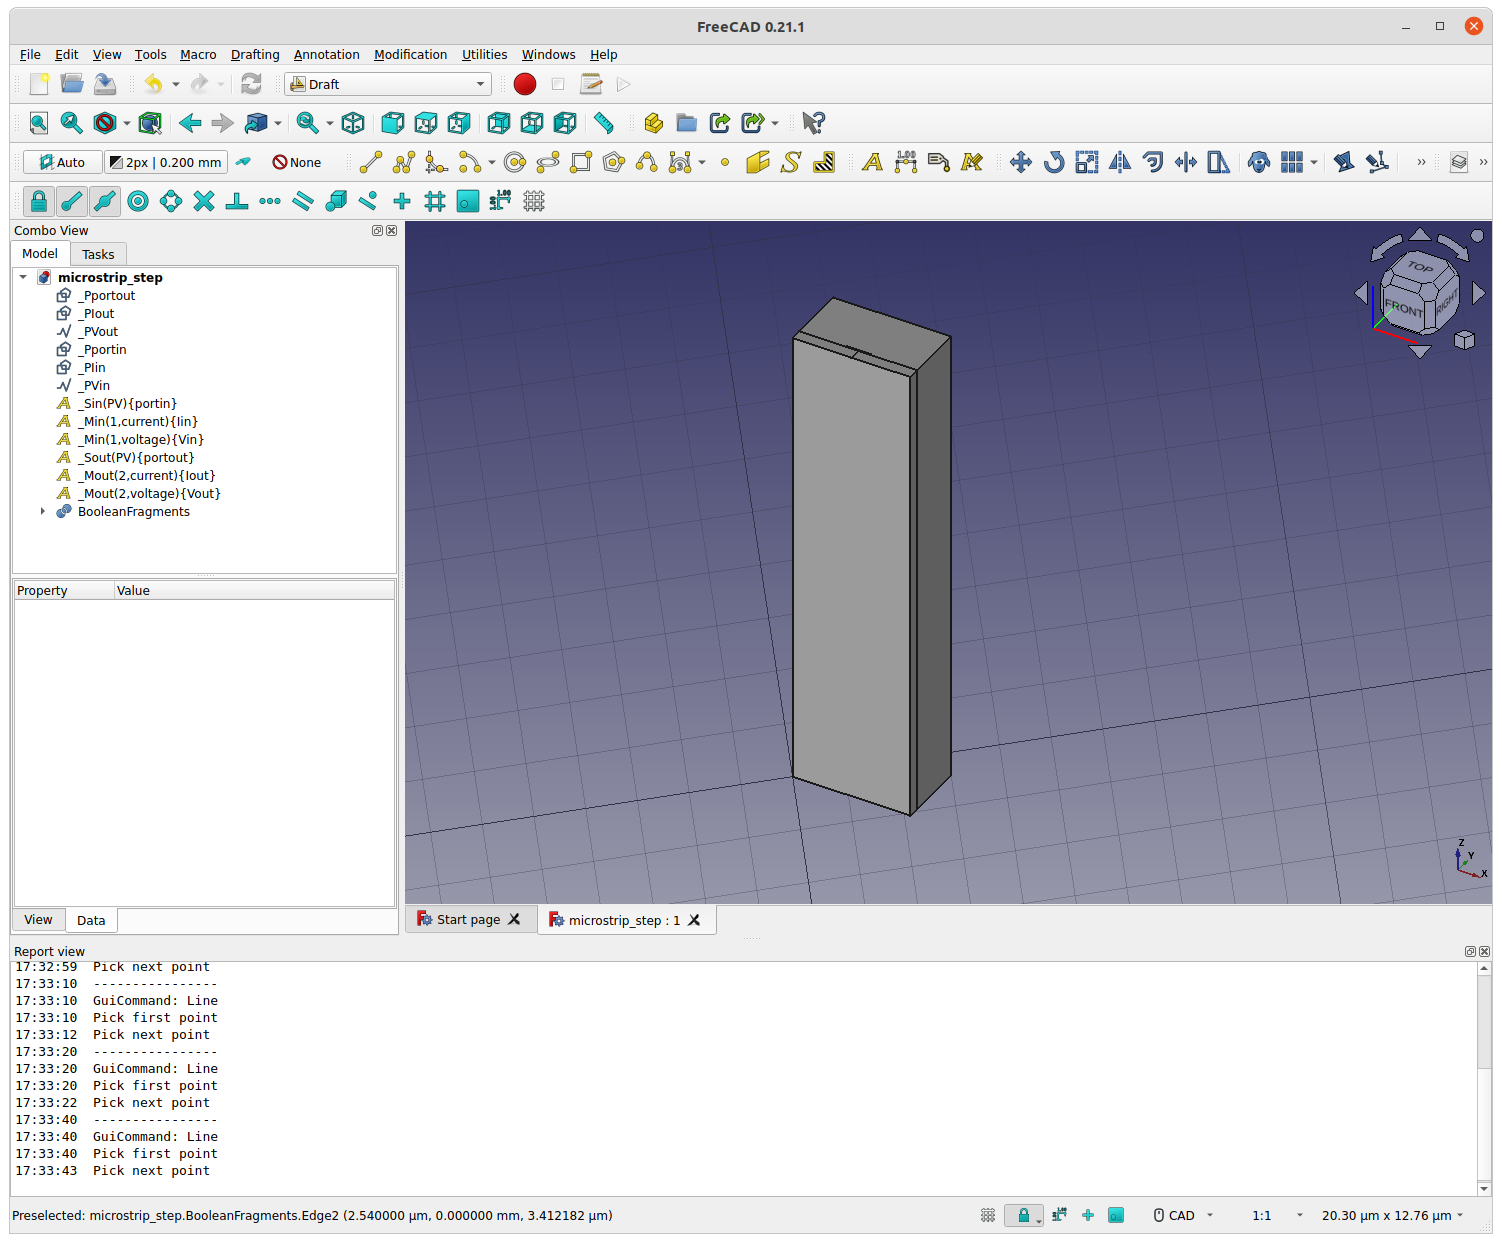
\includegraphics[width=0.75\textwidth]{../tutorials/OpenParEM3D/microstrip_step/screenshots/microstrip3D}
  \caption{Screenshot of the completed 3D setup.}
  \label{fig:microstrip3D}
\end{figure}
\item Save the drawing and exit FreeCAD.
\end{itemize}

\subsubsection{Meshing}
\begin{itemize}
\item Start gmsh and open the saved BREP file.
\item Assign materials by clicking the options tree $\boxplus$\texttt{Geometry}$\rightarrow$$\boxplus$\texttt{Physical Groups}$\rightarrow$$\boxplus$\texttt{Add}$\rightarrow$\texttt{Volume}.
\item In the pop-op window type \texttt{air} then select the yellow dot showing the area of air.  When selected, the dot turns red.  Press the keyboard \texttt{e} and a new pop-up appears.  Click \texttt{Create new `.geo' file}.
\item Change the text from \texttt{air} to \texttt{alumina} then select the yellow dot showing the substrate.  Press the keyboard \texttt{e}.
\item If the mouse does not select the dots, click the red box in the lower left to re-enable mouse input.
\item Since both materials are assigned, press the keyboard \texttt{q} to finish.
\item The default settings for this problem result in port meshes that are not very good with long thin triangles.  To address that, select \texttt{Tools}$\rightarrow$\texttt{Options} to pop up an options control window. Then select \texttt{Mesh}$\rightarrow$\texttt{General}$\rightarrow$\texttt{2D algorithm}$\rightarrow$\texttt{Packing of parallelograms}.  This choice is made simply by trying the various options to see which one produces the best mesh that avoids long thin triangles at the ports.
\item Mesh the geometry by selecting in the options tree click $\boxplus$\texttt{Mesh}$\rightarrow$\texttt{3D}. A screenshot of the mesh is shown in Fig.~\ref{fig:microstrip_mesh}.
\begin{figure}
  \centering
  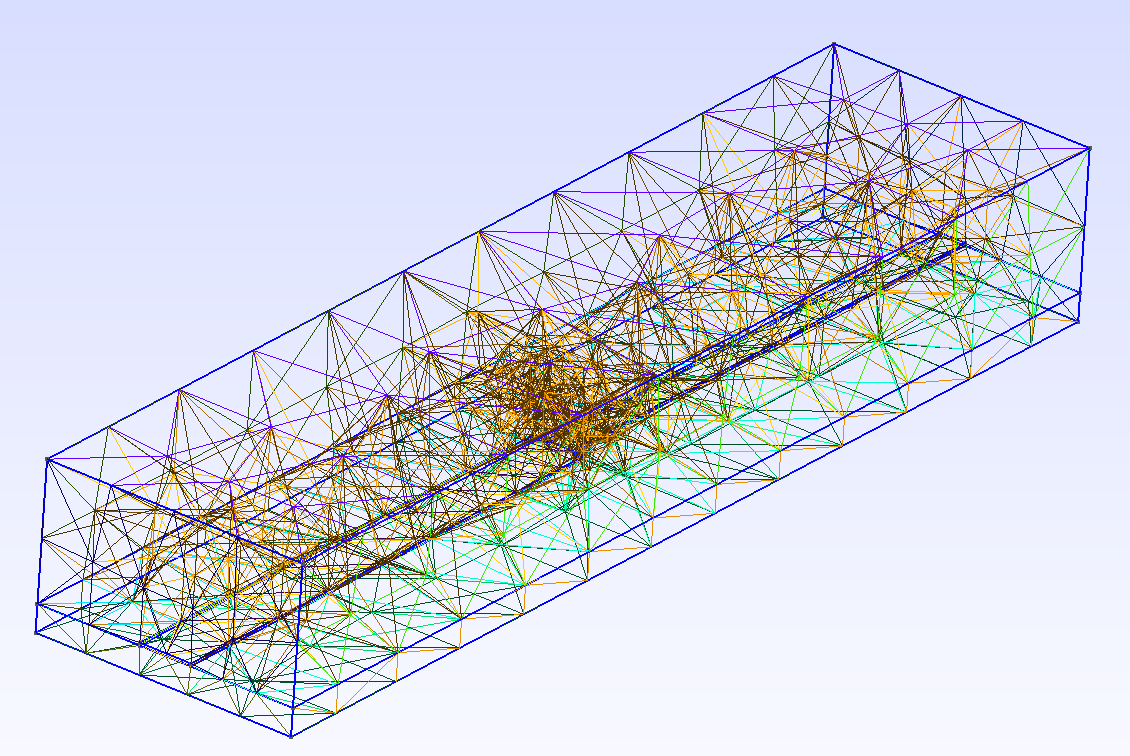
\includegraphics[width=0.75\textwidth]{../tutorials/OpenParEM3D/microstrip_step/screenshots/microstrip_mesh}
  \caption{Screenshot of the meshed microstrip step in width.}
  \label{fig:microstrip_mesh}
\end{figure}
\item Save the meshing options with \texttt{File}$\rightarrow$\texttt{Save Model Options}.  The options file is automatically loaded when loading the \texttt{*.geo} file to enable exactly reproducing a mesh, if needed, or to experiment with different settings based on the previous set.
\item Save the mesh by selecting \texttt{File}$\rightarrow$\texttt{Save Mesh}.
\item Quit gmsh.
\end{itemize}

\subsubsection{Solving}

\begin{itemize}

\item Create the materials file \texttt{local\_materials.txt} in any text editor and set the text contents to
\begin{Verbatim}[fontsize=\small]
#OpenParEMmaterials 1.0
Material
   name=air
   Temperature
      temperature=any
      Frequency
         frequency=any
         er=1.0006
         mur=1
         tand=0
         Rz=0
      EndFrequency
   EndTemperature
   Source
      Constantine A. Balanis, "Advanced Engineering Electromagnetics",
      John Wiley and Sons, 1989, p.79.
   EndSource
EndMaterial

Material
   name=alumina
   Temperature
      temperature=any
      Frequency
         frequency=any
         er=9.8
         mur=1
         tand=0.001
         Rz=0
      EndFrequency
   EndTemperature
   Source
      Generic numbers for testing.
   EndSource
EndMaterial
\end{Verbatim}

\item Create the project control file \texttt{microstrip\_step.proj} in any text editor and set the text contents to
\begin{Verbatim}[fontsize=\small]
#OpenParEM3Dproject 1.0
project.save.fields            true
mesh.file                      microstrip_step.msh
mesh.refinement.limit          0.001
mesh.quality.limit             1000
mesh.order                     3
port.definition.file           microstrip_step_ports.txt
materials.global.path          ./
materials.global.name          //global_materials.txt
materials.local.path           ./
materials.local.name           local_materials.txt
refinement.frequency           high
refinement.iteration.min       5
refinement.iteration.max       40
refinement.required.passes     1
refinement.relative.tolerance  0.01
refinement.absolute.tolerance  1e-06
refinement.variable            S
frequency.plan.point           10e9
reference.impedance            0
\end{Verbatim}

\noindent Adaptive refinement is applied due to the step and the edges of the microstrip lines.  With 3$^{\textnormal{rd}}$-order elements and a fairly dense mesh, extensive refinement is not required, so \texttt{mesh.refinement.limit} is set to 0.001 to avoid excess mesh refinement in areas that do not need it.
See Appendix~\ref{sec:control_file_spec} for a complete list of available keyword/value pairs that can be included in the project control file. Note that the reference impedance in the setup file is set to 0, so no renomalization of the S-parameters is performed.

\item Run OpenParEM3D at the command line with
\begin{Verbatim}[fontsize=\small]
   $ OpenParEM3D microstrip_step.proj
\end{Verbatim}
to run serially with a single core or with
\begin{Verbatim}[fontsize=\small]
   $ mpirun -q --oversubscribe -np 12 OpenParEM3D microstrip_step.proj
\end{Verbatim}
to run in parallel with 12 cores.  Substitute a larger or smaller core number as needed.  The option \verb+--oversubscribe+ is not needed if the number of cores is less than or equal to half the number of available cores.
\item View the 2-port S-parameters with any suitable command with the results looking very much like
\begin{Verbatim}[fontsize=\tiny]
#Touchstone format,DB
#frequency unit,GHz
#number of frequencies,1
#number of ports,2
#S-port 1,net1,not renormalized
#S-port 2,net2,not renormalized
#prior iterations pre-pended by #
#Frequency(GHz),dB(S(1;1)),deg(S(1;1)),dB(S(2;1)),deg(S(2;1)),dB(S(1;2)),deg(S(1;2)),dB(S(2;2)),deg(S(2;2))
#10,-14.3788194129828,-143.036442197428,-0.185196128220973,48.4464694369318,-0.185196128220973,48.4464694369318,-14.3755919817412,59.8969360333806
#10,-14.362668706561,-140.717182087972,-0.185757429822056,48.7203941057591,-0.185757429822056,48.7203941057591,-14.3605686334538,58.1152503635806
#10,-15.0609315968138,-140.446314251543,-0.161152208903268,48.9306989849119,-0.161152208903268,48.9306989849119,-15.0598550941328,58.2646381098206
#10,-14.9451364784807,-137.325796300873,-0.164934958702496,48.9940535036704,-0.164934958702496,48.9940535036704,-14.9442860056249,55.2642922102583
#10,-14.7133374053955,-130.774185096104,-0.172895827590975,49.4685808388707,-0.172895827590975,49.4685808388707,-14.7098431887646,49.664383434521
#10,-15.0736731086306,-126.892681553932,-0.160788555756301,49.8746771388686,-0.160788555756301,49.8746771388686,-15.0675315888474,46.6021770759152
#10,-14.3340642233797,-124.043577116534,-0.186785815594501,50.2794740952806,-0.186785815594501,50.2794740952806,-14.3297637712834,44.5637330342644
#10,-14.8900638973219,-124.283555395446,-0.16673100423588,50.4968103406548,-0.16673100423588,50.4968103406548,-14.8857288440341,45.2485990207109
#10,-15.1144957451646,-119.320411172487,-0.158159711324455,50.6089280321123,-0.158159711324455,50.6089280321123,-15.1098168809666,40.5542876526387
10,-14.9648003515474,-119.345393752942,-0.163069728604374,50.618965517188,-0.163069728604374,50.618965517188,-14.9590784928379,40.6098185523797
\end{Verbatim}
The results prepended by \# are the results at each iteration, and the final result is the last line without the \#.  Results from other computers will show some differences due to the nature of iterative solutions of the Ax=b problem combined with partioning with MPI.

The output from OpenParEM3D shows the results from the 2D port simulations, and the impedances for the input and output ports are 47.59~$\Omega$ and 33.25~$\Omega$, respectively.  Considering just the transmission lines, the return loss from these impedances is 20*log10(abs(33.25-47.59)/(33.25+47.59))=-15.02~dB, which is very close to the computed value of -14.96~dB.  Note also the expected close values for \textbar S11\textbar and \textbar S22\textbar.
\item Start ParaView and open the results file for port 1.
\item Add a filter by selecting \texttt{Filters}$\rightarrow$\texttt{Alphabetical}$\rightarrow$\texttt{Slice}.
\item In \texttt{Plane Parameters} select \texttt{Y Normal}, uncheck \texttt{Show Plane}, and change the y-component of the origin to 0.0002.
\item Click the \texttt{-Y} axis orientation on the tool bar.
\item Change \texttt{Solid Color} to \texttt{gridReE} and change the value shown from \texttt{Magnitude} to \texttt{Y} or \texttt{1}, depending on the version of ParaView.  In the buttons below, change the scale to be symmetric with a range of -4000 to +4000.
\item A screen shot of the resulting Re($E_y$) field just under the microstrip traces is shown in Fig.~\ref{fig:microstrip_ReEy}.
\begin{figure}[H]
  \centering
  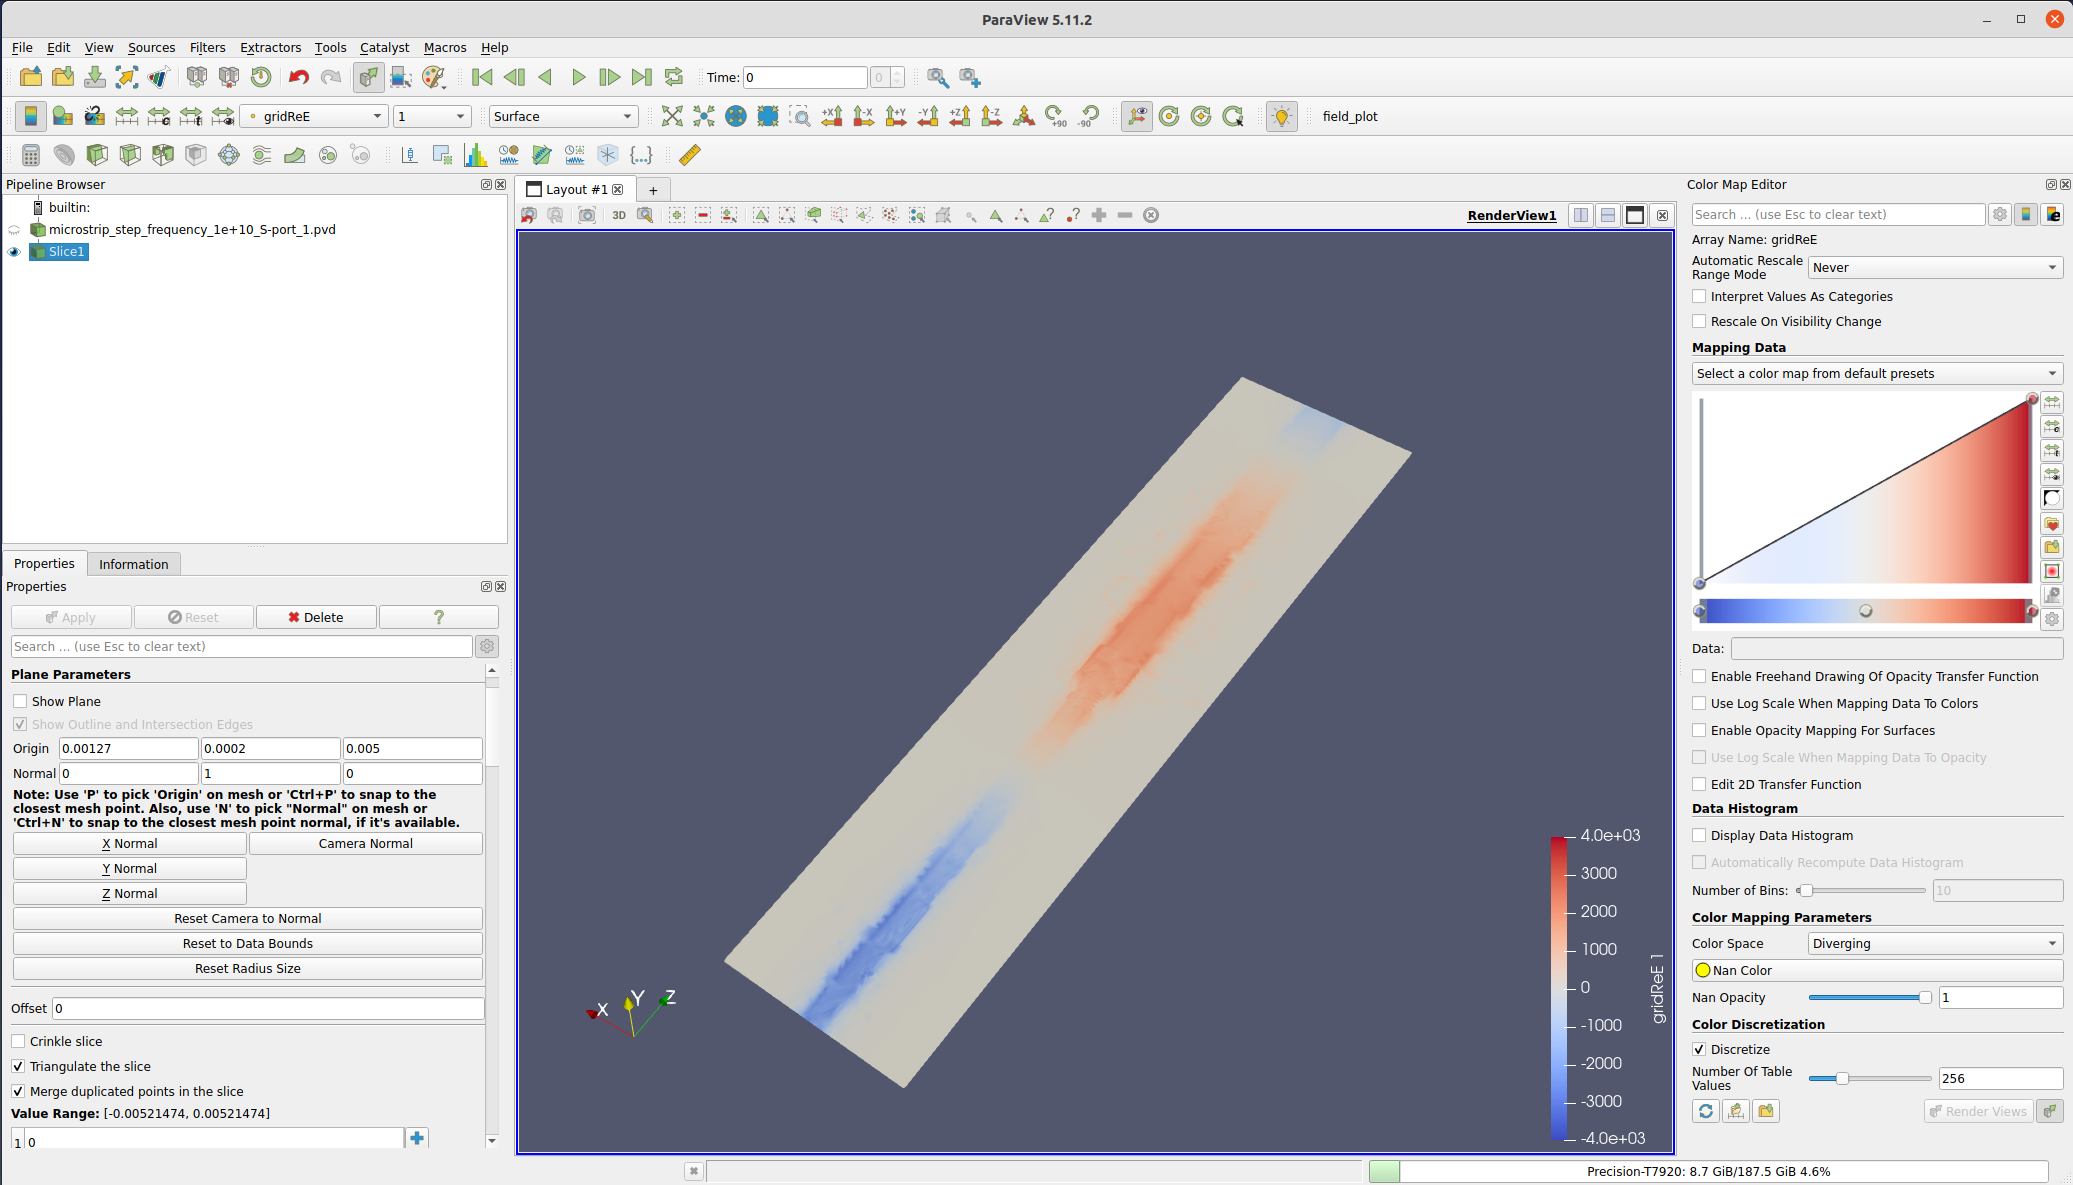
\includegraphics[width=0.75\textwidth]{../tutorials/OpenParEM3D/microstrip_step/screenshots/microstrip_ReEy}
  \caption{Screenshot of Re($E_y$) just under the microstrip lines.}
  \label{fig:microstrip_ReEy}
\end{figure}

\end{itemize}

\subsection{Monopole Antenna}
\label{sec:monpoleantenna}

A monopole antenna with coax feed is constructed and annotated for 1-port S-parameter simulation, meshed, and solved.  The tutorial demonstrates the modeling of round conductors, ports internal to the 3D drawing space, and manually applied boundary conditions [radiation in this tutorial].

\subsubsection{Drawing and Port Annotation}

\begin{itemize}
\item Create a directory for the project called \texttt{monopole\_antenna}.
\item Start FreeCAD, open a new drawing, set preferences [if needed], set the drawing workspace to \texttt{Draft}, and set the drawing plane to \texttt{Top} as outlined in Sec.~\ref{sec:freecad}.
\item Assuming that the prior tutorials have been completed, references to the workspace and specific property boxes are omitted.
\item Draw a multi-sided polygon to represent a circle by selecting \texttt{Drafting}$\rightarrow$\texttt{Polygon}.  Click on the drawing space to start the polygon then another place to complete it.
\item Select the polygon and edit its properties to center it on the origin, set the number of faces to 12, and set the radius to 0.6um to end up with a 6~mm radius in the mesh.
\item Extrude this polygon -20um to represent the pin of the feed coax.  Change its label to \texttt{pin}.
\item Draw another 12-sided polygon with a radius of 2.07um at the origin and extrude it -20um to represent the Teflon of the coax feed.  Change its label to \texttt{dielectric}.
\item Draw another 12-sided polygon with a radius of 2.5um at the origin and extrude it -21um to represent the outer conductor of the coax feed.  Change its label to \texttt{void}. This will eventually be a void to represent metal that also clears a space to place the port at the end of the coax, which must be on the outside facing a void.  The thickness of the outer conductor is somewhat arbitrary.
\item Draw a rectangle that is 100um per side, center it on the origin, then extrude it -0.5um to represent the ground plane for the antenna. Change its label to \texttt{gp}.
\item Save the drawing as \texttt{monopole\_antenna}.
\item The groundplane needs a hole in it to clear the monopole.  Clone \texttt{void}, then select \texttt{gp}, add the clone to the selection, then Boolean cut the clone from \texttt{gp}.  Change the label of the new object to \texttt{groundplane}.
\item Yes, there is a lot of back-and-forth between the \texttt{Draft} and \texttt{Part} workspaces.
\item Draw a 12-sided polygon with a radius of 1um at the origin and extrude it +15um to represent the dipole with an approximate resonant frequency of 5~GHz. Change its label to \texttt{monopole}.
\item Draw a rectangle that is 200um per side, center it on the origin, extrude it 200um, then shift the resulting box in the z-direction -100um to represent air. Change its label to \texttt{air}.
\item Right click in the drawing area and select \texttt{Draw style}$\rightarrow$\texttt{Wireframe}.  The view should look like that in Fig.~\ref{fig:monopole_building_blocks}.
\begin{figure}
  \centering
  \begin{subfigure}{0.75\textwidth}
     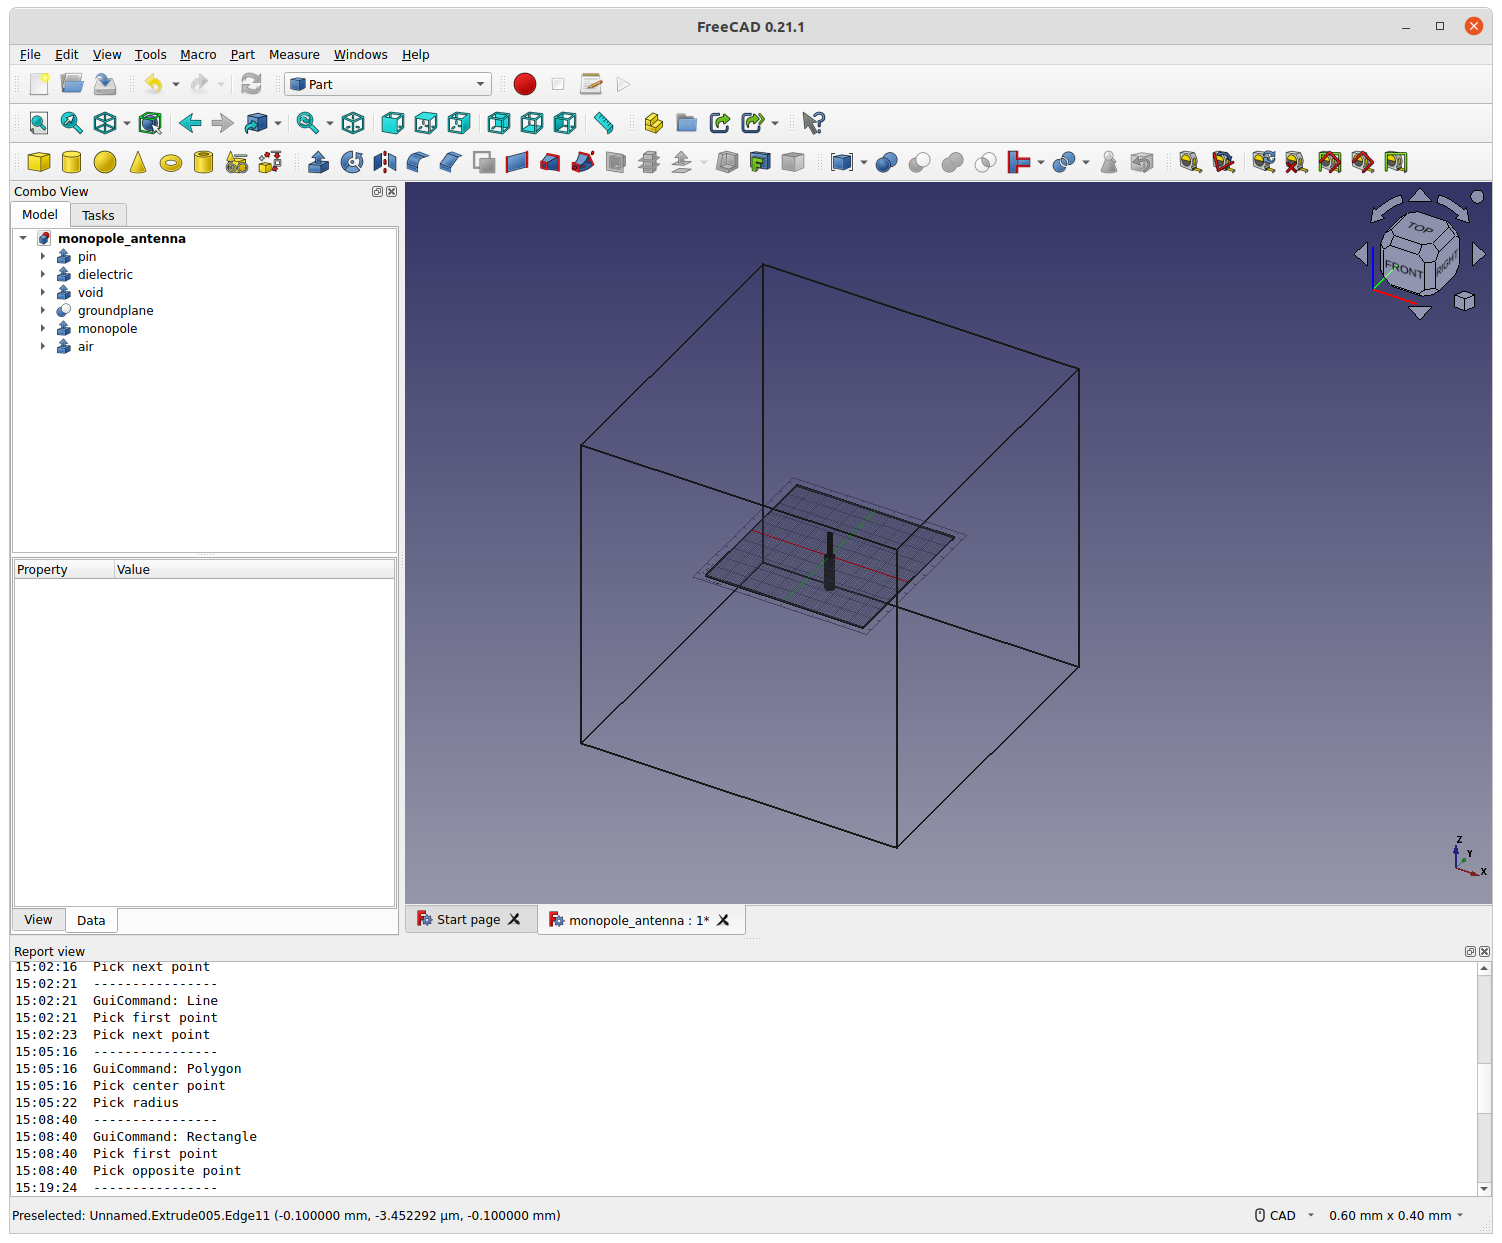
\includegraphics[width=\linewidth]{../tutorials/OpenParEM3D/monopole_antenna/screenshots/monopole_building_blocks}
     \caption{View of all}
  \end{subfigure}
  \par\bigskip
  \begin{subfigure}{0.75\textwidth}
     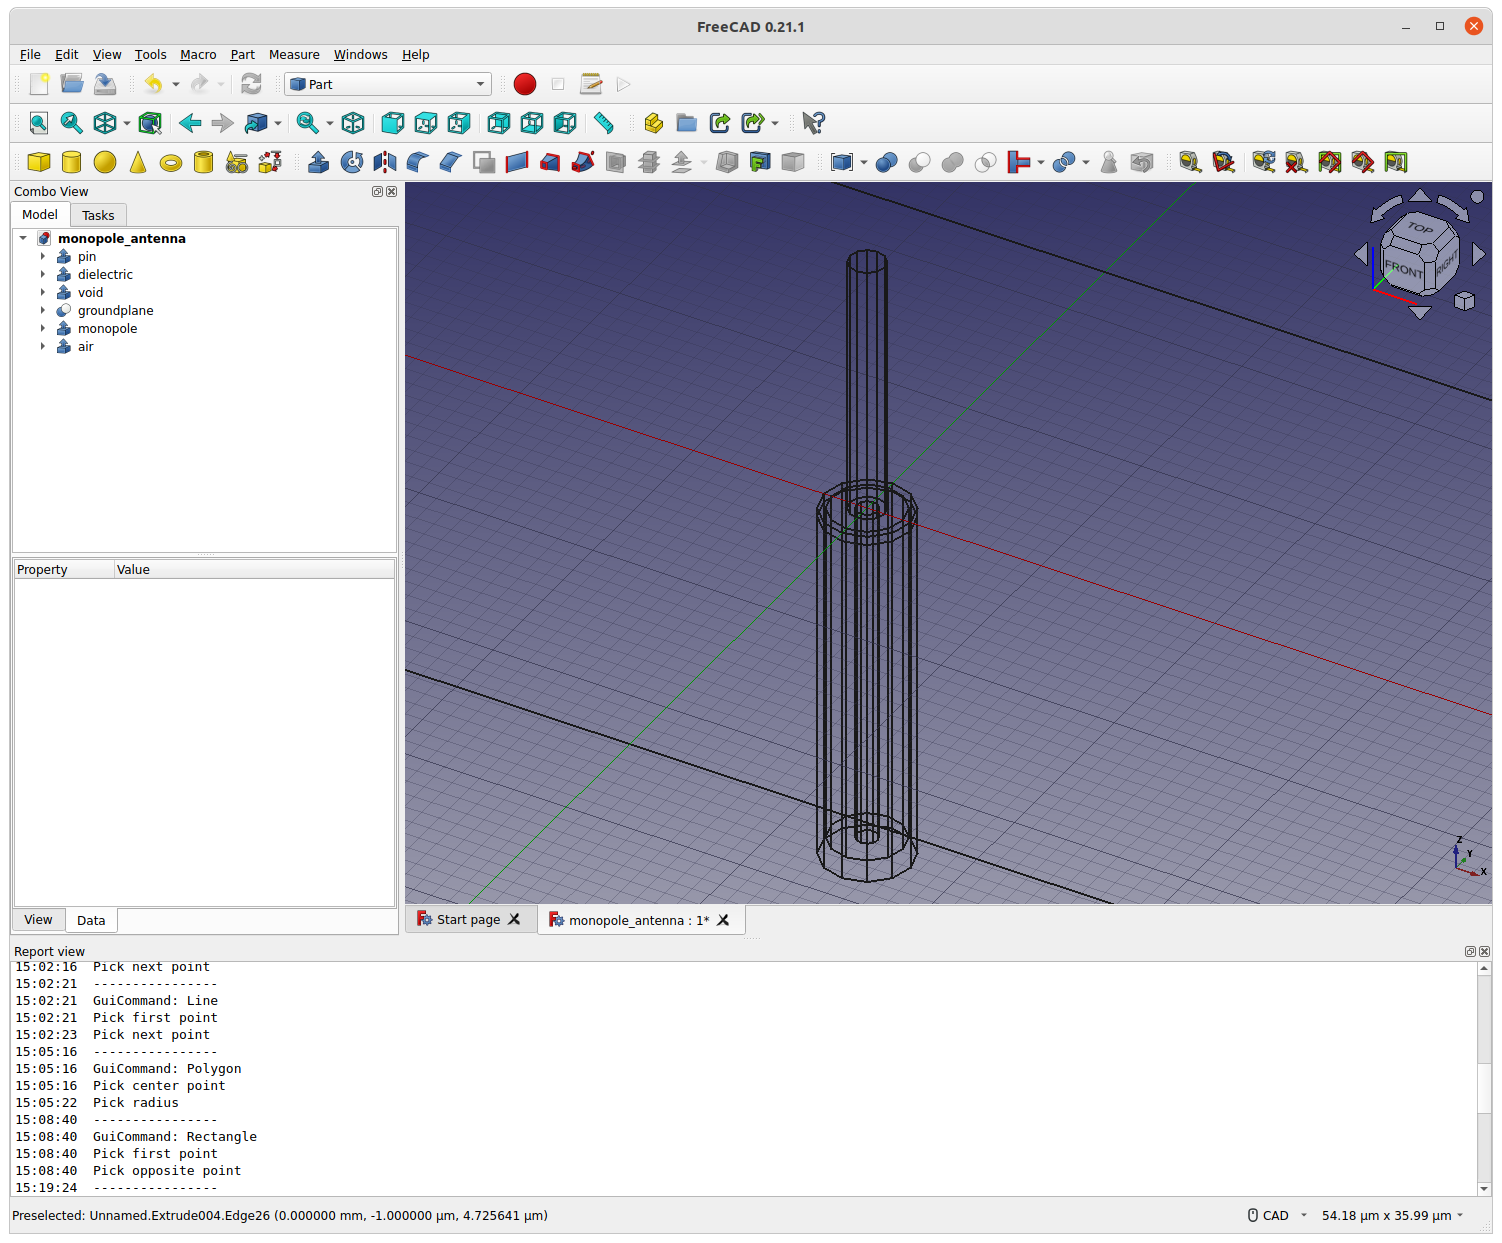
\includegraphics[width=\linewidth]{../tutorials/OpenParEM3D/monopole_antenna/screenshots/monopole_zoom}
     \caption{Zoom towards center}
  \end{subfigure}
  \caption{Monopole building blocks.}
  \label{fig:monopole_building_blocks}
\end{figure}
\item Right click in the drawing area and select \texttt{Draw style}$\rightarrow$\texttt{As is}.
\item Hide \texttt{air} and \texttt{void}.
\item Set the view to \texttt{Bottom}, select one of the visible surfaces, and set the drawing plane to that surface.
\item Draw a 12-side polygon to match the size of \texttt{dielectric}.  Verify that the radius is 2.07~$\mu$m.  Change its label to \texttt{\_Pport}.  This is the port on the end of the coax line.
\item Draw a line from the lowest vertex of \texttt{dielectric} to the lowest vertex of \texttt{pin}.  Verify that the length is 1.47~$\mu$m.  Change its label to \texttt{\_Pv}.  This is the voltage integration line on the port.
\item Set \texttt{air} to visible.
\item In the \texttt{Draft} workspace, select each of the six sides of the air box in turn, make that side the drawing plane, and draw a rectangle covering the complete side of the air box by snapping to the corners.  Do this six times and change the labels to \texttt{\_Pfront}, \texttt{\_Pback}, \texttt{\_Pleft}, \texttt{\_Pright}, \texttt{\_Ptop}, and \texttt{\_Pbottom}.  These six rectangles completely cover the air box.  Note that in a slightly more advanced usage, one side can be set as the drawing plane, and both rectangles parallel to that drawing plane can be drawn, so only three changes of the drawing plane are strictly necessary.
\item Select \texttt{dielectric} and cut \texttt{pin} from it.  Change its label to \texttt{teflon}.  Because of the void, the teflon piece has a metal pin embedded within it.
\item Select \texttt{air} and cut \texttt{void} from it.
\item Select the resulting object and cut \texttt{groundplane} from it.
\item Select the resulting object and cut \texttt{monopole} from it.
\item Select the resulting object and add \texttt{teflon} to the selection, then create a Boolean fragment.
\item Select the Boolean fragment and export a BREP file called \texttt{monopole\_antenna.brep}.
\item For the port, add text items with the labels \texttt{\_Sin(PV){port}} \texttt{\_Min(1,voltage){v}}.
\item For the radiation boundary conditions, add text items with the labels \texttt{\_Bfront(radiation){front}}, \newline\texttt{\_Bback(radiation){back}}, \texttt{\_Bleft(radiation){left}}, \texttt{\_Bright(radiation){right}}, \newline\texttt{\_Btop(radiation){top}}, and \texttt{\_Bbottom(radiation){bottom}}.
\item Run the macro "OpenParEM3D\_save.py" and save the results in \texttt{monopole\_antenna\_ports.txt}.  Verify that there are no errors.
\item Save the file and exit FreeCAD.
\end{itemize}

For layouts like this with thin structures, it can be very beneficial to take the time to draw nested cylinders or boxes to enclose the active structure that start a little larger than the active structure and progressively get bigger.  This helps the mesher focus the mesh in the neighborhood of the active structure and to limit long thin mesh elements.  The payoff for the extra drawing effort is faster convergence to a more accurate solution.  For this example, nested structures are not utilized for simplicity.

\subsubsection{Meshing}

The box boundary is 0.33$\lambda$ in air from the dipole at 1~GHz, which is too close for a 1$^{\textnormal{st}}$-order radiation boundary condition, so the computed results at very low frequencies will see a small impact.  At the expected resonance near 5~GHz, the boundary is 1.7$\lambda$ away, which is good for a 1$^{\textnormal{st}}$-order boundary.  At 10~GHz, the wavelength is 30~mm in air, and assuming the use of 4$^{\textnormal{th}}$-order finite elements, maximum mesh edge lengths of 0.75$\lambda$ can be accurately modeled without adaptive mesh refinement.  The setup sets the maximum edge length to 22.5~mm, then adaptive mesh refinement is confined to the near field by setting \texttt{mesh.refinement.fraction} to 0.001.

\begin{itemize}
\item Start gmsh and open the saved BREP file.
\item Assign the two volumes with their respective materials of \texttt{air} and \texttt{teflon}.
\item Set the maximum mesh edge length with \newline\texttt{Tools}$\rightarrow$\texttt{Options}$\rightarrow$\texttt{Mesh}$\rightarrow$\texttt{General}$\rightarrow$\texttt{Max element size}$\rightarrow$0.0225.
\item Create the 3D mesh and save it.
\item Save the mesh options with \texttt{File}$\rightarrow$\texttt{Save Model Options}.
\item Exit gmsh.
\end{itemize}

\subsubsection{Solving}

The solution for the monopole antenna is performed in two steps to minimize the number of files generated.  In the first step, the mesh is optimized at 10~GHz and the S-parameters are swept starting at 1~GHz.  The optimized mesh is saved, and in the second step, a second simulation is performed at 4.75~GHz using the optimized mesh to produce 3D volume fields, far fields, and computed antenna metrics.

\begin{itemize}

\item Create the materials file \texttt{local\_materials.txt} in any text editor and set the text contents to
\begin{Verbatim}[fontsize=\small]
#OpenParEMmaterials 1.0
Material
   name=air
   Temperature
      temperature=any
      Frequency
         frequency=any
         er=1.0006
         mur=1
         tand=0
         Rz=0
      EndFrequency
   EndTemperature
   Source
      Constantine A. Balanis, "Advanced Engineering Electromagnetics",
      John Wiley and Sons, 1989, p.79.
   EndSource
EndMaterial

Material
   name=teflon
   Temperature
      temperature=any
      Frequency
         frequency=any
         er=2.2
         mur=1
         tand=0.0
         Rz=0
      EndFrequency
   EndTemperature
   Source
      generic teflon
   EndSource
EndMaterial
\end{Verbatim}

\item Create the project control file \texttt{monopole\_antenna.proj} in any text editor and set the text contents to
\begin{Verbatim}[fontsize=\small]
#OpenParEM3Dproject 1.0
project.save.fields            false
mesh.file                      monopole_antenna.msh
mesh.refinement.fraction       0.001
mesh.quality.limit             1e4
mesh.save.refined              true
mesh.order                     4
port.definition.file           monopole_antenna_ports.txt
materials.global.path          ./
materials.global.name          //global_materials.txt
materials.local.path           ./ 
materials.local.name           local_materials.txt
refinement.frequency           plan
refinement.iteration.min       5
refinement.iteration.max       40
refinement.required.passes     1
refinement.relative.tolerance  0.01
refinement.absolute.tolerance  1e-06
refinement.variable            S
frequency.plan.point.refine    10e9
frequency.plan.linear          1e9,10e9,0.1e9
reference.impedance            0
\end{Verbatim}
\noindent This control file calls for mesh optimization and S-parameters but does not save any fields or compute any antenna metrics.

\item Run OpenParEM3D at the command line with
\begin{Verbatim}[fontsize=\small]
   $ mpirun -q --oversubscribe -np 12 OpenParEM3D monopole_antenna.proj
\end{Verbatim}

\item The computed S-parameters are shown in Fig.~\ref{fig:monopole_S}.
\begin{figure}[H]
  \centering
  \begin{subfigure}{0.5\textwidth}
     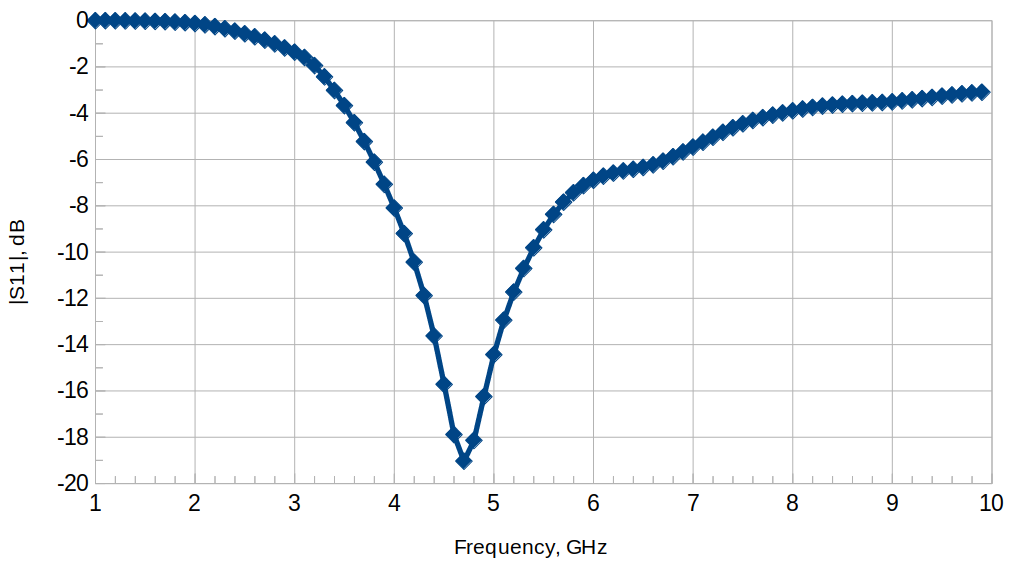
\includegraphics[width=\linewidth]{../tutorials/OpenParEM3D/monopole_antenna/screenshots/monopole_mag}
     \caption{Magnitude.}
  \end{subfigure}
  \par\bigskip
  \begin{subfigure}{0.5\textwidth}
     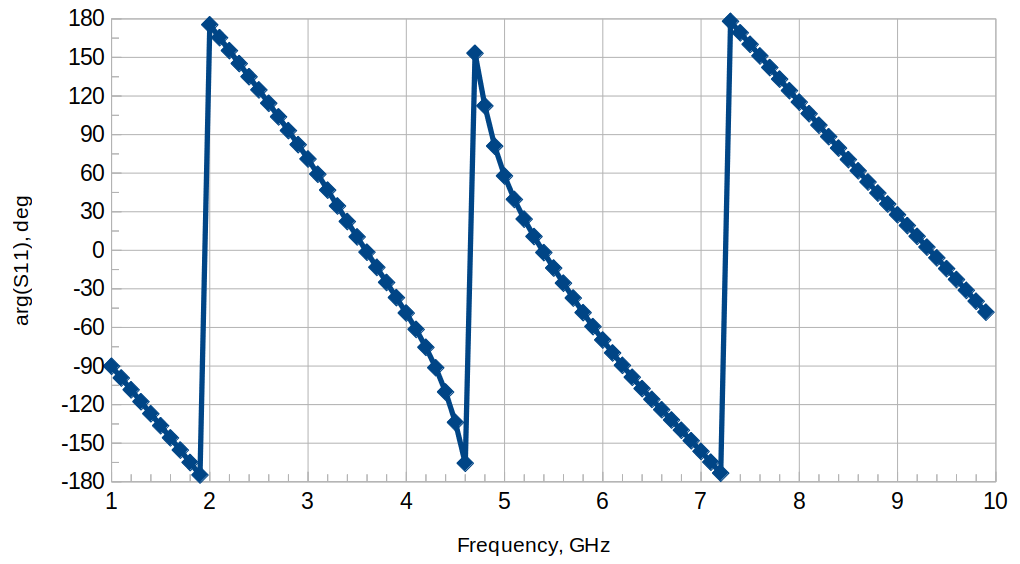
\includegraphics[width=\linewidth]{../tutorials/OpenParEM3D/monopole_antenna/screenshots/monopole_phase}
     \caption{Phase.}
  \end{subfigure}
  \caption{Computed S-parameters for a monopole antenna.}
  \label{fig:monopole_S}
\end{figure}

\item Create a second project control file \texttt{monopole\_antenna\_fields.proj} in any text editor and set the text contents to
\begin{Verbatim}[fontsize=\small]
#OpenParEM3Dproject 1.0
project.save.fields            true // false
mesh.file                      refined_monopole_antenna.msh // monopole_antenna.msh
mesh.refinement.fraction       0.001
mesh.quality.limit             1e4
mesh.save.refined              false // true
mesh.order                     4
port.definition.file           monopole_antenna_ports.txt
materials.global.path          ./
materials.global.name          //global_materials.txt
materials.local.path           ./
materials.local.name           local_materials.txt
refinement.frequency           none // plan
refinement.iteration.min       5
refinement.iteration.max       40
refinement.required.passes     1
refinement.relative.tolerance  0.01
refinement.absolute.tolerance  1e-06
refinement.variable            S
//frequency.plan.point.refine    10e9
//frequency.plan.linear          1e9,10e9,0.1e9
frequency.plan.point           4.75e9
reference.impedance            0
antenna.plot.3D.pattern        q=G
antenna.plot.2D.pattern        q1=G,plane=xy,latitude=15
antenna.plot.2D.pattern        q1=G,plane=xz,rotation=180
\end{Verbatim}
\noindent This control file pulls in the previously optimized mesh and solves for S-parameters, far-field radiation patterns, and antenna performance metrics.

\item Run OpenParEM3D at the command line with
\begin{Verbatim}[fontsize=\small]
   $ mpirun -q --oversubscribe -np 12 OpenParEM3D monopole_antenna_fields.proj
\end{Verbatim}
\noindent Note that this project can be run simultaneously with the project defined by \texttt{monopole\_antenna.proj} after it has completed mesh optimization and produced the final version of the mesh file \texttt{refined\_monopole\_antenna.msh}.  It is not necessary to wait for the first project file to complete its sweep before running the second project file.

\item The computed antenna metrics are saved to the file \texttt{monopole\_antenna\_fields\_FarField\_results.csv}, copied here as
\begin{Verbatim}[fontsize=\small]
#prior iterations pre-pended by #
#S-port,frequency,gain,directivity,radiation efficiency
1,4750000000,4.08382872576697,4.11573461423741,0.992680318001095
\end{Verbatim}
\noindent As shown in the file, the gain is 4.08~dB, the directivity is 4.12~dB, and the radiation efficiency is 99.3\%.  Since the simulation has no dielectric or conductor losses, the radiation efficiency is very high at resonance.  In such a simualation, it would not be unexpected for the efficiency to exceed 100\% by a small amount due to the approximate nature of a finite element solution.  For an infinite ground plane, the gain would be a slightly over 5, but the finite ground plane allows some energy behind the ground plane, as visible in the backside lobes in Fig.~\ref{fig:monopole_G}, reducing the gain to 4.08~dB.

\item View the computed far fields with ParaView using the files saved in the directory \texttt{ParaView\_monopole\_antenna\_fields\_FarField}.

Open the file \texttt{G\_4.75e+09\_SP1}, change \texttt{Solid Color} to \texttt{G}, set \texttt{Normal Array} to \texttt{normals}, and set \texttt{Specular} to \texttt{1}.  The 3D far-field gain is shown in Fig.~\ref{fig:monopole_G}(a), where the influence of the finite ground plane can be seen on the field.

Open the files \texttt{slice\_G\_4.75e+09\_xz\_0\_0\_SP1} and \texttt{slice\_G\_4.75e+09\_xz\_0\_0\_SP1} to show slices cut through the 3D pattern as shown in Fig.~\ref{fig:monopole_G}(b).  View all together to ensure that the slices are as expected, and de-select various plots to explore the slices in isolation.

\begin{figure}[H]
  \centering
  \begin{subfigure}{0.33\textwidth}
     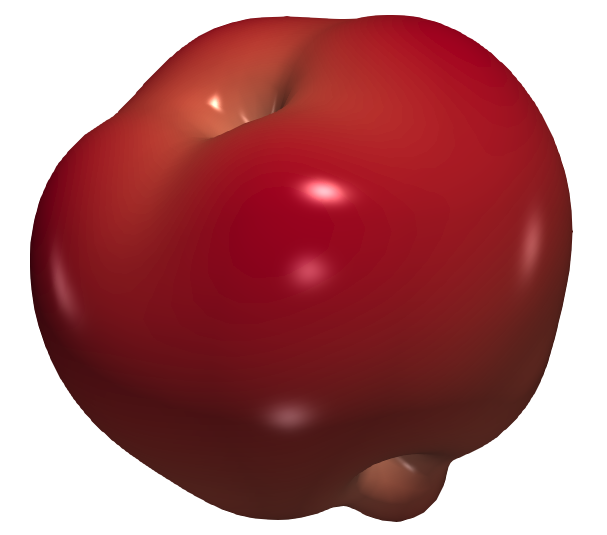
\includegraphics[width=\linewidth]{../tutorials/OpenParEM3D/monopole_antenna/screenshots/monopole_3D_gain}
     \caption{Isotropic gain.}
  \end{subfigure}
  \begin{subfigure}{0.33\textwidth}
     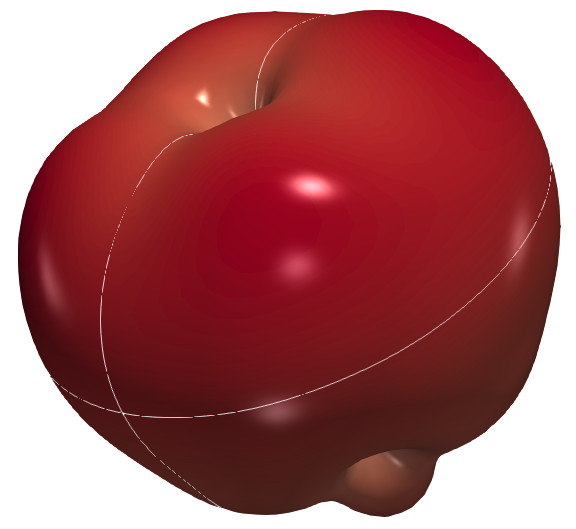
\includegraphics[width=\linewidth]{../tutorials/OpenParEM3D/monopole_antenna/screenshots/monopole_3D_gain_slices}
     \caption{Isotropic gain with slices.}
  \end{subfigure}
  \caption{Isotropic gain at 4.75 GHz.}
  \label{fig:monopole_G}
\end{figure}

\item Reports for the slices are in the directory \texttt{Report\_monopole\_antenna\_fields\_FarField}.  These can be viewed by executing
\begin{Verbatim}[fontsize=\small]
   $ evince radiation_pattern_G_4.75e+09_xy_15_0_SP1.pdf &
   $ evince radiation_pattern_G_4.75e+09_xz_0_0_SP1.pdf &
\end{Verbatim}
\noindent The reports are shown in Fig.~\ref{fig:monopole_G_slices}.  Note that the gains and directivities shown on the slice report are the maximum values on that slice.  The maximum values for the 3D pattern overall are given in the far-field results file, \texttt{monopole\_antenna\_fields\_FarField\_results.csv} for this project.

\begin{figure}[H]
  \centering
  \begin{subfigure}{0.408\textwidth}
     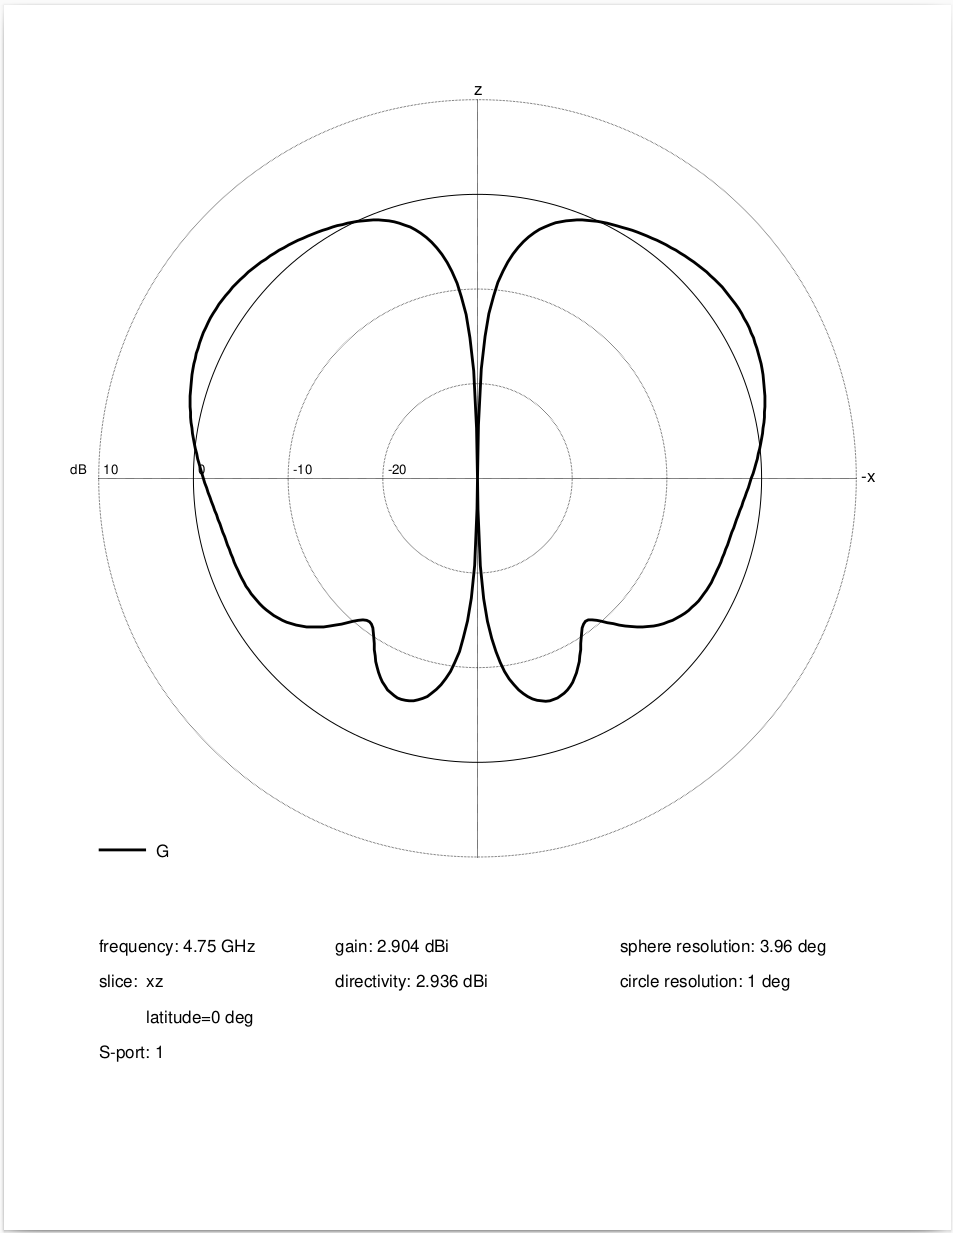
\includegraphics[width=\linewidth]{../tutorials/OpenParEM3D/monopole_antenna/screenshots/radiation_pattern_G_4.75e+09_xz_0_180_SP1}
     \caption{Slice through the x-z plane.}
  \end{subfigure}
  \begin{subfigure}{0.41\textwidth}
     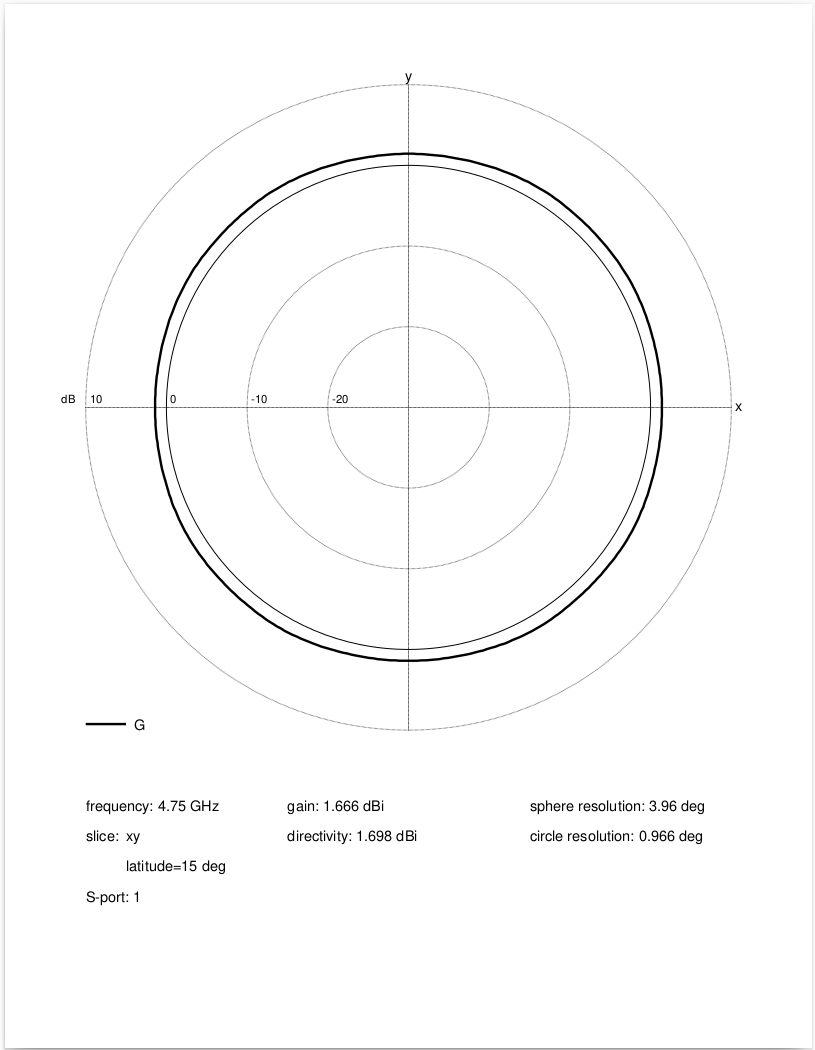
\includegraphics[width=\linewidth]{../tutorials/OpenParEM3D/monopole_antenna/screenshots/radiation_pattern_G_4.75e+09_xy_15_0_SP1}
     \caption{Slice through the x-y plane at latitude 15$^\circ$.}
  \end{subfigure}
  \caption{Isotropic gain slice reports at 4.75 GHz.}
  \label{fig:monopole_G_slices}
\end{figure}

\item Field plots throughout the 3D volume can be set up and viewed in ParaView.  Taking slices through the volume, the real part of the electric field computed at 4.75~GHz on the x-z plane is shown in Fig.~\ref{fig:monopole_ReE}, while Fig.~\ref{fig:monopole_ReH} shows the real part of the magnetic field on the x-y plane at z=4~mm.

\begin{figure}[H]
  \centering
  \begin{subfigure}{0.6\textwidth}
     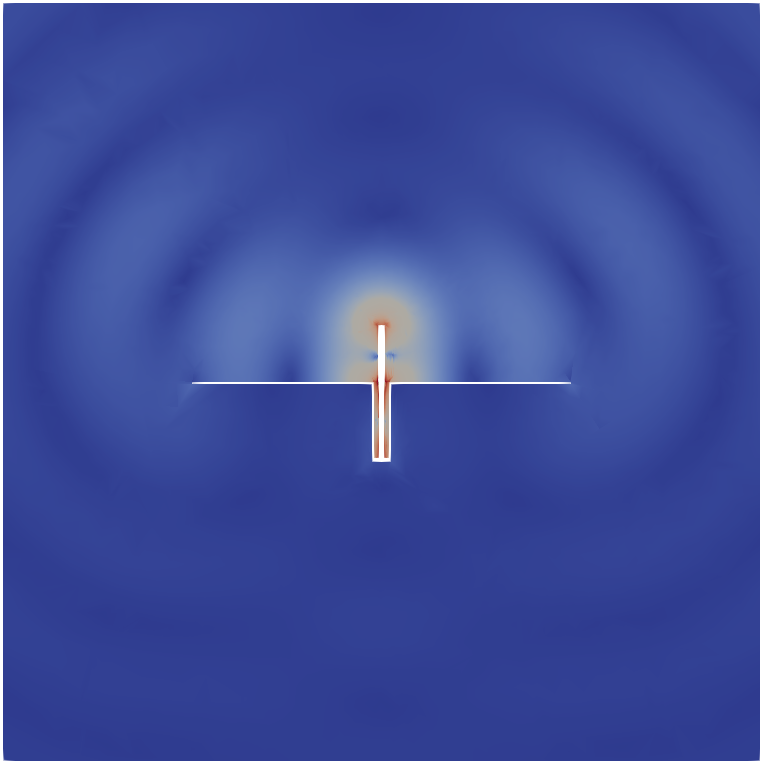
\includegraphics[width=\linewidth]{../tutorials/OpenParEM3D/monopole_antenna/screenshots/Eplane_4p75GHz}
     \caption{$|\textnormal{Re}(\overline{E})|$}
  \end{subfigure}
  \par\bigskip
  \begin{subfigure}{0.6\textwidth}
     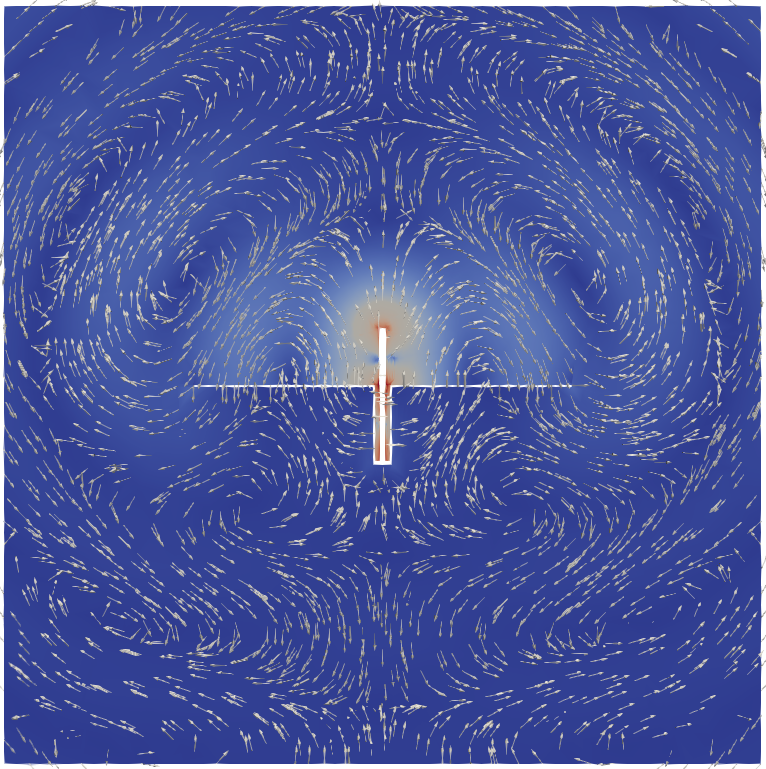
\includegraphics[width=\linewidth]{../tutorials/OpenParEM3D/monopole_antenna/screenshots/Eplane_vector_4p75GHz}
     \caption{$\textnormal{Re}(\overline{E})$}
  \end{subfigure}
  \caption{Real part of the electric field at 4.75~GHz.}
  \label{fig:monopole_ReE}
\end{figure}
\begin{figure}[H]
  \centering
  \begin{subfigure}{0.6\textwidth}
     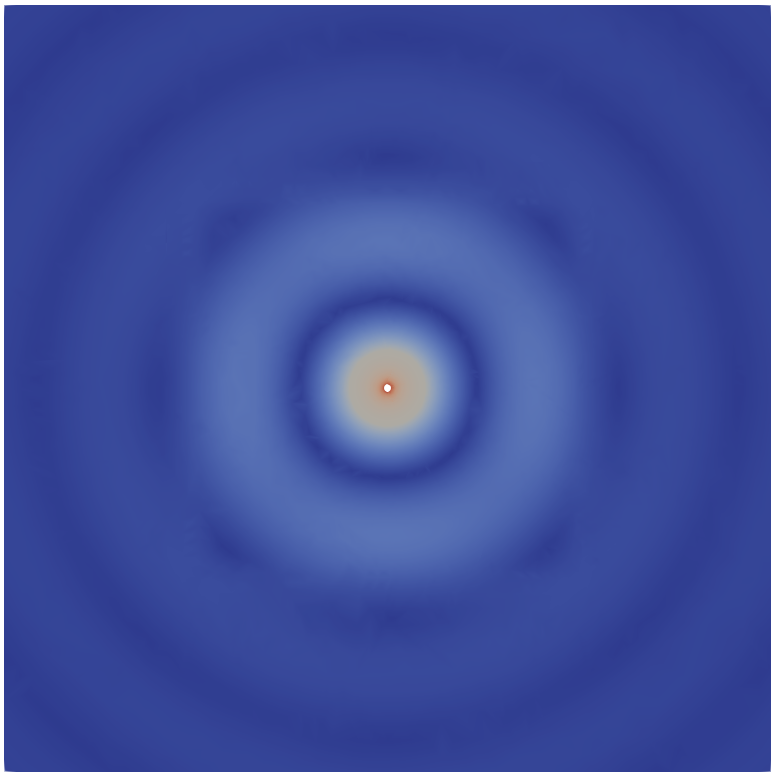
\includegraphics[width=\linewidth]{../tutorials/OpenParEM3D/monopole_antenna/screenshots/Hplane_4p75GHz}
     \caption{$|\textnormal{Re}(\overline{H})|$}
  \end{subfigure}
  \par\bigskip
  \begin{subfigure}{0.6\textwidth}
     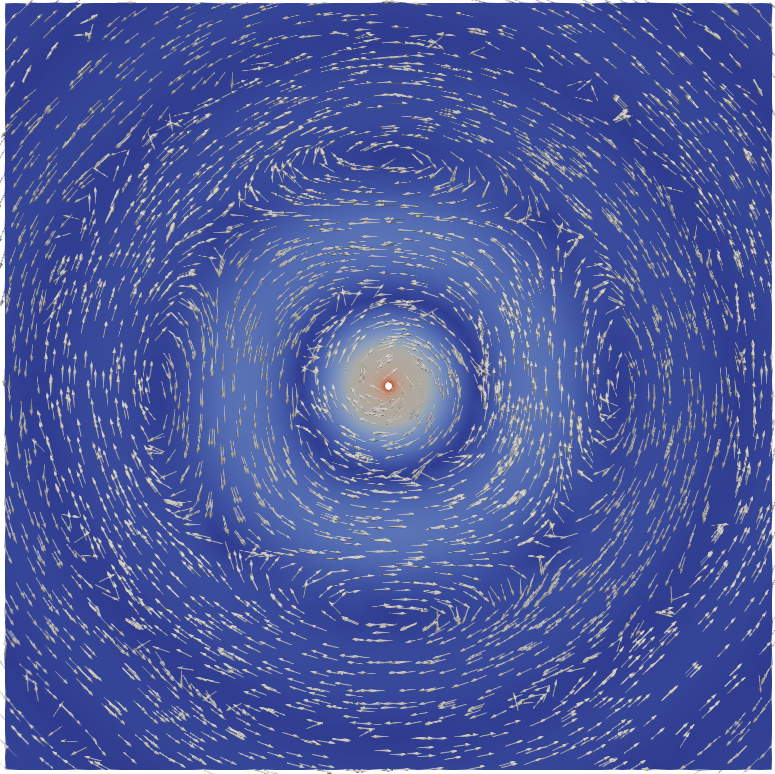
\includegraphics[width=\linewidth]{../tutorials/OpenParEM3D/monopole_antenna/screenshots/Hplane_vector_4p75GHz}
     \caption{$\textnormal{Re}(\overline{H})$}
  \end{subfigure}
  \caption{Real part of the magnetic field at 4.75~GHz.}
  \label{fig:monopole_ReH}
\end{figure}


\end{itemize}

\section{Techniques}

\subsection{Wave Ports}

The math behind OpenParEM3D assumes that the 3D electromagnetic fields at the ports represent transmission lines or waveguides, meaning that the field dependence along the direction orthogonal to the port ($\hat{n}$) has the dependence $e^{-\gamma n}$.  Ports must be placed on the ends of transmission lines or waveguides that are long enough to ensure that the electromagnetic fields have settled into their modal configurations.  How long is long enough?  A reasonable rule-of-thumb is to make the transmission lines or waveguides twice as long as the lateral extent of the fields, which may or may not align with the dimensions of the port.  For critical work, it could be reasonable to run the problem a second time with a longer transmission lines or waveguides to see if the S-parameters change.  Visual inspection of the fields from a completed solution can also help determine if the transmission lines or waveguides for the ports are long enough.  \textit{Failure to ensure that the port transmission lines or waveguides are long enough will result in incorrect answers with no warning from OpenParEM3D.}

In some setups, the parasitic effects from short port transmission lines or waveguides produce minimal error and may be acceptable.  When the port transmission lines or waveguides are too short, the 2D field imposed at the port carries into the 3D space, where the 3D fields adjust to create the needed parasitics to satisfy Maxwell's equations.  These parasitics are not correct, but their impact may be small enough to ignore.  It is up to the user to decide if the parasitics can be negelected.

\subsection{Multimode Ports With Unequal $\gamma$}

For non-driven ports, an absorbing boundary condition is applied to absorb energy propagating towards the port from within the 3D space.  The absorbing boundary condition (ABC) is dependent on the complex propagation constant, $\gamma$, selected for the 2D ABC, and only one $\gamma$ can be applied at a given port.  If more than one mode is present, such as for differential pairs, the largest $\gamma$ is used.  If the $\gamma$s for the other modes are significantly different, then they will suffer some reflection that puts energy back into the 3D space that affects the solution.  The larger the reflection, the worse the effect on accuracy.  OpenParEM3D detects when the span of $\gamma$ is too large, prints an error, and exits.  However, there may be cases where the impact on accuracy is not significant, so the option to override the error detection is available.  To allow OpenParEM3D to simulate cases with multimode ports with non-equal $\gamma$, set the keyword \texttt{solution.check.homogeneous} to \texttt{false}.  This limitation is expected to be addressed with a PML absorbing boundary, when implemented.

\subsection{Finite Element Order}

The finite element order is set with the keyword/value pair \texttt{mesh.order N} in the project control file.  \texttt{N} can be any integer and sets the order of the polynomial approximating the field in each finite element.  All elements in a mesh have the same element order.

Higher values for \texttt{N} have potential advantages due to the polynomial accommodating larger field variations within any given element.  The advantages of higher order include:
\begin{itemize}
\item Greater accuracy for a given mesh size.
\item Smaller mesh size for a given accuracy.
\item Better accuracy for frequency sweeps.
\item Smoother fields for visualization.
\end{itemize}
\noindent However, there are also disadvantages of higher order:
\begin{itemize}
\item Slower run times for a given mesh size.
\item Larger memory consumption.
\item Harder convergence in 2D simulations, although order-ramping in OpenParEM2D may offer a fix, when implemented.
\end{itemize}
\noindent The disadvantages ramp quickly with increasing \texttt{N}.
OpenParEM3D does not currently support GPU computing, which can alleviate the disadvantages of higher \texttt{N}.

\subsubsection{Guidelines}

Experience to date suggests the following guidelines for selecting \texttt{N}:
\begin{itemize}
\item Assuming a simulation runs to completion in an acceptable time, higher \texttt{N} is always better than lower \texttt{N}.
\item Avoid \texttt{N=1}.  Adaptive refinement is required and the number of iterations is just too great.  Improved adaptive meshing algorithms might address this issue.
\item Generally, \texttt{N=3} and \texttt{N=4} are good options.
\item Choose the largest \texttt{N} that allows a quick first iteration when using adaptive refinement.  What qualifies as \textit{quick} depends on mesh size, the speed of the computer, and user patience.
\item In the first iteration, if the 2D port solutions take more than a few seconds or require a very large iteration limit [like 100,000], then decrease \texttt{N}.  Conversely, if the first iteration is very quick, then try increasing \texttt{N}.  Note that very slow convergence for the 2D simulations can be caused by a poor mesh at the ports, so it is important to ensure that the mesh has good triangulation at the ports by avoiding long thin triangles.
\item Problems with relatively smooth fields, such as those using waveguide, greatly benefit from larger \text{N}.  For some problems, adaptive refinement may not be needed.
\item Problems with sharp edges, such as edge-coupled stripline, benefit from a highly refined mesh around the edges.  To keep run times reasonable, it can be beneficial to use \texttt{N=2}.
\item If using iterative refinement, and the number of iterations is very large, then an increase in \texttt{N} could be in order.  Conversely, if only a couple of iterations are needed, then a smaller \texttt{N} could be useful to force an increase in the number of iterations to help uncover potential areas where additional refinement would improve the S-parameters.
\item Dense meshes with element edges that are small compared to the wavelength should use smaller $N$ to avoid numerical issues due to over-meshing as discussed in Sec.~\ref{sec:overmeshing}.
\item Meshes with large areas where there is little field variation should use smaller $N$ to avoid numerical issues due to over-meshing as discussed in Sec
.~\ref{sec:overmeshing}.
\item ParaView supports \texttt{N} up to 6.  If ParaView will be used to review field plots, then keep \texttt{N} to 6 or fewer.
\end{itemize}

\subsubsection{Sinusoidal Fields}

If the fields in a given problem are known to have a sinusoidal or near-sinusoidal distribution, such as the transition and far-field regions of antennas, the finite element order can be selected along with a constraint on the mesh generation to accelerate convergence with AMR or to help avoid AMR entirely.  Table~\ref{table:sinusoidal} shows a few cases of error vs. wavelength vs. order.  For example, by restricting the maximum element edge to 0.5$\lambda$ during meshing, 3$^{\textnormal{rd}}$-order elements can be used to achieve $\pm$0.81\% error without AMR in the sinusoidal and near-sinusoidal areas.  AMR can then focus on the remaining areas for quicker convergence and better accuracy.

\begin{table}
\small
\caption{Polynomial Fitting Accuracy for Sinusoids}
\begin{center}
\begin{tabular}{|c|c|c|}
\hline
Order & Wavelength Fraction & Error, \% \\
\hline
2 & 0.25 & $\pm$0.19 \\
2 & 0.5	 & $\pm$2.8 \\
3 & 0.25 & $\pm$0.027 \\
3 & 0.5 & $\pm$0.81 \\
3 & 0.666 & $\pm$4.0 \\
3 & 1     & $\pm$18 \\
4 & 0.5   & $\pm$0.10 \\
4 & 0.75  & $\pm$1.1 \\
\hline
\end{tabular}
\end{center}
\label{table:sinusoidal}
\end{table}

\subsection{Over-Meshing}
\label{sec:overmeshing}

All computations involve finite precision, and it is possible to demand more precision from a computer than it can provide, in which case accuracy will degrade.  For finite element programs such as OpenParEM3D, excess precision requirements occur when a problem has far more mesh density than that required to accurately solve a problem.  This is called \textit{over-meshing}.  

Consider an example of a problem minimally meshed such that the geometry is barely but accurately captured by the mesh and that first-order finite elements are used to solve the problem with adaptive mesh refinement.  At the first iteration, the computed result will have poor accuracy because the linear finite elements cannot capture the curvature of the fields.  Adaptive refinement subdivides the mesh in areas of high error, meaning areas where the linear approximation is poor, thereby improving the ability of the linear elements to describe the field.  This process continues with additional refinements until the linear approximation provides a reasonable fit to the field curvature in all areas.

Now, what happens if adaptive refinement continues after the approximation of the linear finite elements already provides a good fit to the field curvature?  Certainly, the fit of the field gets better.  However, a problem begins to develop where the improvement starts to push down to lower decimal places.  So with hypothetical numbers, the first iteration provides a 10\% improvement, the second 1\%, third 0.1\%, fourth 0.01\%, etc.  Eventually, the required precision runs out of decimals for accurate calculation, and the computed solution starts losing accuracy.  More iterations just make it worse.

The same effect can happen by choosing finite element orders that provide too much variability than that required by the problem.  For example, a perfectly linear field structure would be accurately described by a linear finite element and a second-order finite element.  However, for the second-order element, the computation must accurately zero out the quadratic term, which requires extra digits of precision.  Once a field is accurately captured by a finite element order, going substantially higher in order can actually decrease accuracy.

The key is to avoid relying on excessive numerical precision by not over-meshing a problem.  The concept is the same whether low- or high- order finite elements are used.  Generally, the higher the order of the finite elements, the less dense the mesh needs to be to avoid over-meshing.

Best practice is to simply mesh the problem with minimal settings and then let adaptive mesh refinement or stepping up the finite element order converge the solution to engineering accuracy then stopping. This practice also results in minimal run time.  The goal is really to just not "play it safe" by targeting excessively high accuracies.  

\subsubsection{identifying over-meshing}

Over-meshing is most likely to occur during adaptive mesh refinement, and its onset can generally be identified by  the behaviors of the relative S error and the H error metric in the file \texttt{projectname\_iterations.txt}.  For the relative S error, over-meshing produces inconsistent convergence with increasing iteration count, where the solution may appear to be converging then a large jump in the error occurs, then the cycle repeats.  For the H error metric, over-meshing is identifiable when the metric stops improving with iteration count, moving down and up, without making steady progress towards a lower error.  

\subsubsection{mesh edge length/wavelength in element}

OpenParEM3D provides an output during execution to help with determining settings to avoid over-meshing, and this is the \texttt{mesh edge length/wavelength in element} line.  At each frequency, the length of each edge of every element is divided by the wavelength in the material in which the element resides, then the minimum and maximum fractions are reported.  So for example, the output will show something like
\begin{Verbatim}[fontsize=\small]
    mesh edge length/wavelength in element: shortest=0.000965796 longest=0.00846018
\end{Verbatim}
In this example, the longest element is short compared to the wavelength at just 0.85\%.  The field cannot change very much in such a small element, so low-order finite elements are appropriate, and care must be taken to not force too many iterations.

\subsubsection{concentrated fields}

Geometries that have concentrated fields in small areas that are located within large spaces result in areas with limited field variations.  These should generally use lower-order finite elements to prevent high-order elements from causing numerical problems modeling fields with low spatial variation away from the area of concentrated fields.  An example of such a case is a step in width of microstrip.

\subsubsection{diffuse fields}

Geometries with fields varying throughout the problem space strongly benefit from using higher-order elements.

\subsubsection{small mesh elements}

Initial meshes with very small maximum length elements reported by \texttt{mesh edge length/wavelength in element} should generally use lower-order finite elements.

\subsubsection{large mesh elements}

Initial meshes with large maximum length elements reported by \texttt{mesh edge length/wavelength in element} can take advantage of higher-order finite elements to accelerate convergence with adaptive mesh refinement.

\subsubsection{mesh.refinement.fraction}

The setting \texttt{mesh.refinement.fraction} determines how many mesh elements are refined at each pass of adaptive mesh refinement.  For problems with fields varying across the entire problem space, a larger value such as the default 0.005 is a good choice to avoid excessive iteration count.

For problems where most of the field variation is concenterated in a small percentage of the volume, the default value for \texttt{mesh.refinement.fraction} can lead to over-meshing.  The reason is that \newline\texttt{mesh.refinement.fraction} sets the number of elements to refine irrrespective of the element errors, so if only a few elements have high errors, then refinement spills over to low-error elements, which is bad for numerical accuracy.  For problems with concentrated fields, a good value for \texttt{mesh.refinement.fraction} is 0.001 to 0.002.  With such a small refinement fraction, the user must take care to avoid early termination in the first few iterations.

\subsubsection{refinement.required.passes}

Sometimes, the S-parameter relative tolerance can be met before the field accuracy is sufficient when a mesh refinement does not happen to significantly impact the S-parameters.  A protection against this is to set \texttt{refinement.required.passes} to 2 or more.  However, this can lead to over-meshing, especially for larger problems.

\subsubsection{refinement.absolute.tolerance}

Use of \texttt{refinement.absolute.tolerance} can drive adaptive mesh refinement to excessive numbers of iterations if it is set too low.  It is most useful in helping to avoid early termination when a mesh adaptation does not happen to produce a large change in the S-parameters, so the relative convergence criteria is met too early.  Instead of setting \texttt{refinement.required.passes} to 2 or more, \texttt{refinement.absolute.tolerance} can be set to a moderate error and \texttt{refinement.variable} to \texttt{SandH} to avoid an early termination.

\subsubsection{1$^{\textnormal{st}}$-order elements}

1$^{\textnormal{st}}$-order elements are not the most efficient way to solve a problem, but they are probably the safest in avoiding over-meshing.  New users may choose to use 1$^{\textnormal{st}}$-order elements to gain experience before moving on to higher-order elements.  Experienced users may find it useful to re-run a questionable case with 1$^{\textnormal{st}}$-order elements to double-check results.

\subsection{FreeCAD Port Alignment to Mesh}

The port must align exactly to the mesh.  In cases where the port does not fall naturally on geometric features, simply include the port in the selection while creating the Boolean fragments object for exporting a BREP file.  During meshing, gmsh will force mesh elements to follow the port outline.

Including voltage integration paths in the Boolean fragments object will also force mesh edges to follow the path, and this may slightly improve the simulation accuracy.

\subsection{Mesh Re-Use}

When using adaptive mesh refinement, the refined mesh can be saved by setting \texttt{mesh.save.refined true} in the project control file.  This can be used to advantage when multiple frequency sweeps are expected.  A first simulation pass can be done to just adaptively refine the mesh.  Then, the project control file can be copied, the mesh changed to the refined mesh, refinement disabled, and the frequency sweep added.  Multiple frequency sweeps can be make without having to re-refine the mesh.  For example, a relatively coarse sweep can be made, then finer sweeps can be done to fill in sharp resonance peaks and nulls.

The refined mesh is in the MFEM native format rather than the gmsh format.  To view the MFEM mesh directly, glvis can be used.

\subsection{Adaptive Mesh Refinement Convergence}

There are two controls for deciding when to terminate adaptive mesh refinement: convergence on S with a relative error and convergence on the H field with an absolute error.  One or the other or both can be used as the convergence criteria.

\subsubsection{S with relative error}

In the project control file, set \texttt{refinement.variable S} and \texttt{refinement.relative.tolerance reltol}, where \texttt{reltol} is set to some value such as 0.01.

Converging exclusively on S with a relative error can result in early termination of adaptive refinement.  Sometimes a round of mesh refinement improves the fields but does not significantly change the S-parameters, leading to termination while the field accuracy is still low.  To protect against this, the project control file can require more than one consecutive iterations using \texttt{refinement.required.passes N} to meet the relative convergence criteria.  However, this can turn into a bit of a guessing game: what relative convergence to set and how many consecutive iterations are needed.  An alternative strategy is to set a minimum number of iterations using \texttt{refinement.iteration.min N} to ensure that at least $N$ iterations are performed before the convergence criteria can be accepted.

\subsubsection{H with absolute error}

In the project control file, set \texttt{refinement.variable SandH}, \texttt{refinement.relative.tolerance reltol}, and \texttt{refinement.absolute.tolerance abstol}.  Set \texttt{reltol} to a large value such as 0.1 such that it very easy to meet the convergence criteria on S.  Set \texttt{abstol} to a value such as 1e-06.  Iterations will proceed until both convergence criteria are met, and since S is easy, then the criteria on the field error becomes the ultimate gating limit.

The adaptive mesh refinement algorithm calculates an absolute error metric on the H field.  Setting the convergence criteria so that the field error becomes the gating limit ensures that the fields reach a good level of refinement.  The downside is that if \texttt{abstol} is set too tight, extra iterations may be made even though the S-parameters may be converged, and excess iterations can also impact accuracy through over-meshing.

\subsubsection{S with relative error \textit{and} H with absolute error}

Use the \texttt{SandH} refinement option as above, but set \texttt{reltol} to a value such as 0.01.  Use an \texttt{abstol} such as 1e-06.  Set \texttt{refinement.required.passes 1}.

Effectively, adaptive refinement continues while the field error is high, preventing early termination when the relative error on S does not change much.  After the fields reach a certain level of refinement, then iteration continues, if needed, until the S-parameters converge on the relative error.

\subsubsection{S with relative error \textit{or} H with absolute error}

This option is included for completeness, but it may not be useful in general.

\subsection{Conductor Loss}

Conductor losses are added with polygons defined on each surface to convert from the default perfect electric conductor (PEC) boundary to some other conductor.  Until additional scripting is available in FreeCAD to automate this, it can be very tedious to draw these except for the simplest of cases.

If all metals are the same, then there is an option to change the default boundary condition from PEC to a defined material, such as copper.  To make this change, add the keyword/value pair \newline\texttt{materials.default.boundary some\_metal} to the project control file, where \texttt{some\_metal} is a conductor defined in either the local or global material databases.  Other boundary conditions can still be applied to override the default boundary condition.

\subsection{Antennas}

Much of the volume that is meshed and solved for an antenna is the freespace between the antenna and the radiation boundary condition.  Since OpenParEM3D has a 1$^{\textnormal{st}}$-order radiation boundary condition, the boundary must be placed about 1$\lambda$ or more from the antenna at the lowest simulation freqeuncy to avoid reflections.  The field must be well-modeled throughout the volume to avoid reflections from poorly modeled regions.  In other words, the fields must be well-resolved throughout the 3D volume.

Since it is known that the fields must be well-modelled everywhere, it is good practice to not rely exclusively on AMR to resolve the fields in the transition and far-field areas.  Since the fields are close to or are sinusoidal in these regions, higher order finite elements along with a constrained mesh size can ensure that the fields are accurately represented in the transition and far-field areas.  For example, if the mesher is set to produce a mesh with no edge longer than 1/2$\lambda$, then Table~\ref{table:sinusoidal} shows that a 3$^{\textnormal{rd}}$-order finite element can model the transition and far-fields with $\pm 0.8\%$ accuracy without AMR, and then AMR is only required in the near field near the antenna.  This can accelerate AMR to a more consistent final solution.

If this strategy is used, then it is important to be careful with the setting for \texttt{mesh.refinement.fraction}.  Since the mesh is dominated by transition and far-field mesh elements and since AMR works by subdividing the \texttt{mesh.refinement.fraction} of the mesh elements with the highest error, if \texttt{mesh.refinement.fraction} is set too high, then the subdivisions will spill over from the near field to the transition and far-field regions and create overly dense mesh where it is not needed, impacting both run time and solution quality as discussed in Sec.~\ref{sec:overmeshing}. When using the strategy outlined in this section, keeping \texttt{mesh.refinement.fraction} to a small value, such as 0.001, helps keep AMR focussed on the near field where it is needed. 

\subsection{OpenParEM2D Run Time with MPI}

OpenParEM3D runs OpenParEM2D at the wave ports, and with MPI parallel processing, an efficiency issue occurs with OpenParEM2D.  With MPI, the 3D problem is subdivided and spread across many processors as described in Sec.~\ref{sec:files}.  Generally, the surface areas representing wave ports are a small fraction of the overall 3D problem, so when a large number of processors are specified to \texttt{mpirun}, only a small percentage of them are involved with solving the 2D problem with OpenParEM2D.  However, all the processors must still communicate to solve the problem, so for OpenParEM2D, the MPI overhead of communication increases but the computational power does not. 

When running OpenParEM2D standalone, increasing the number of processors reduces run time until the computer saturates its bandwidth.  When running OpenParEM3D, increasing the number of processors reduces the 3D run time [until the computer saturates], but the OpenParEM2D run times while being run from OpenParEM3D will generally \texttt{increase} even for small numbers of processors.

The overall run time of a 3D problem is dominated by the 3D solve time, not the 2D port solve times.  So while OpenParEM2D suffers a reduction in efficiency, the impact on overall run times is negligible.  However, it can be disconcerting to see the port solves slowing down as the number of processors applied for MPI increases.

\subsection{OpenParEM2D Convergence}

The first step in solving a 3D problem is to solve the 2D eigenvalue problem for the fields and propagation constants at the wave ports.  Since these calculations are full-wave electromagnetic simulations, they can become problematic if they are failing to converge since that stalls the 3D simulation.  Scenarios leading to issues with 2D wave port convergence are described in the following sections.

\subsubsection{Poor Mesh Quality}

Since the 2D simulations are eigenvalue problems, they are more susceptible to poor mesh quality that the 3D simulation.  The output from OpenParEM2D shows the mesh quality at the port, and if the mesh quality is too low (i.e. a large number), then convergence can become very slow.  There are two remedies for this issue: re-mesh to improve the mesh quality at the ports, or decrease the finite element order since high-order elements generally require better mesh quality.

\subsubsection{Large Frequency Step}

Once the 2D simulations successfully complete the first time, the complex propagation constants are stored and used as initial guesses for the next 2D solve.  If the frequencies are closely spaced, then the initial guess is good and the next 2D solve is very quick without convergence issues.  However, if the step is too large, then the initial guess is not as good and convergence issues may occur.  The remedy in this case is to increase the frequency density.

A special case of a large frequency step is when adaptive mesh refinement occurs at a high frequency followed by a frequency sweep starting at a very low frequency.  If convergence at the low frequency is proving difficult, then adaptive refinement can be added at lower frequencies to step down the frequency so that the initial guess is better.  For example, suppose a problem is adaptively refined at 50~GHz with a subsequent sweep starting at 0.1~GHz.  The complex propagation constant at 50~GHz is used as the initial guess at 0.1~GHz, for a 500:1 step down in frequency.  To reduce the size of the step, adaptive mesh refinement at 50~GHz can be followed by adaptive mesh refinement at 5~GHz and then additionally at 0.5~GHz so that the maximum step down in frequency for the initial guess is never more than 10.  [In a case like this, to avoid excessive refinement and very long run times, the convergence tolerance can be relaxed since multiple rounds of adaptive refinement are applied and good accuracy will still be obtained.]

\subsection{MPI and Iterative Solvers}

MPI works by dividing a matrix by rows and spreading them across multiple cores.  Exactly how the split is done depends on the current loading of the computer, so there is variability from run-to-run.  The cores communicate with each other with packets of information and the timing of these also depend on loading, and the order of execution can change from run-to-run.  OpenParEM3D uses iterative solvers for the linear solves of $\overline{E}$ and $\overline{H}$, and the progression of the iterations changes slightly because the data used at each iteration changes due to the variation in the data split and the timing of MPI data packets.  The net result is that the answers produced by OpenParEM3D change slightly from run-to-run.

A low-accuracy simulation demonstrates higher variation from run-to-run than a high-accuracy simulation.  This behavior can be used to build confidence that a solution is converged by re-running the simulation with a different number of cores and seeing how much the answer changes.  Changing the number of cores forces a change in the split of the matrices across cores and has more effect on the computed results.  If the number of cores is not changed, it is possible that the split is identical with similar timings so that the final result does not actually change much.

\subsection{Companion Tool builder}

A companion tool called \textit{builder} helps to quickly build projects for straight sections of some common transmission line and waveguide types. Builder is primarily a tool for optimization of dimensions and materials for characteristic impedance using OpenParEM2D.  However, it includes the option for providing a length to extrude the 2D cross-section into a 3D object. The target uses are calculations of the effect of the conductor losses on delay and generation of S-parameter files for use in circuit simulations with transmission lines or waveguides.
A simple text file with keyword/value pairs describes the physical aspects of the problem to be solved, then builder constructs all of the needed files for OpenParEM3D with the exception of the mesh, which still must be generated in gmsh.  However, in gmsh the materials are already defined, so the process can be as simple as opening the geo file, meshing, then exiting.  The template proj file can be touched up with the remaining specifics for a given simulation. Builder is documented in "builder\_User\_Manual.pdf".

\appendix

\newpage
\section{Control File Specification}
\label{sec:control_file_spec}

OpenParEM3D is controlled by a text file consisting of keyword/value pairs.  The rules for setting up the control file are listed below.
\begin{itemize}[nosep]
  \item The first line of the file must be \verb+#OpenParEM3Dproject 1.0+
  \item One keyword/value pair per line
  \item Except for file names, each keyword has a default value
  \item Keyword/value pairs can appear in the file more than once, and excepting frequency.plan.* and antenna.plot.pattern, the last entry is the one that is used.  Note: No error message or warning is issued when keyword values are overwritten.
  \item All units are MKS: meter, Ohms, Hz, S/m, Celsius.
  \item Angles are in degrees.
\end{itemize}

\tabcolsep=0.05cm
\small
\begin{longtable}[c]{|lccp{8cm}|}
    \hline
    \textbf{Keyword} & \textbf{Value} & \textbf{Default} & \textbf{Description} \\
    \hline
    \endfirsthead
    \hline
    \textbf{Keyword} & \textbf{Value} & \textbf{Default} & \textbf{Description} \\
    \hline
    \endhead
    project.calculate.poynting   & bool   & false & Calculate the Poynting vector (power flow) \\
    project.save.fields          & bool   & false & Save the vector field results for viewing with ParaView \\
    mesh.file                    & string &       & File name of the mesh file \\
    mesh.order                   & int    & 1     & Order of the finite elements \\
    mesh.save.refined            & bool   & false & Save the mesh for re-use in a later run \\
    mesh.refinement.fraction     & double & 0.005 & Maximum fraction of the mesh to refine at each iteration \\
    mesh.quality.limit           & double & 20    & Limit above which a fatal error is triggered. Typically has to be set higher \\
    port.definition.file         & string &       & File name for the boundary condition/port definition file \\
    materials.global.path        & string & ../   & Path to a global materials file serving as a library.  Can also be blank or ./ for the local directory \\
    materials.global.name        & string & global\_materials & File name for the global materials file \\
    materials.local.path         & string & ./    & Path to a local materials file. Can also be blank. \\
    materials.local.name         & string & local\_materials & File name for the local materials file \\
    materials.check.limits       & bool   & true  & Check the material values against range limits \\
    materials.default.boundary   & string & PEC   & Default material to use for unspecified boundaries.  PMC and metals, such as copper, from the materials library are valid entries \\
    refinement.frequency         & string & highlow & Sets the frequency or frequencies on which adaptive mesh refinement is applied.
                                                   
                                                   Options: 
                                                   \begin{itemize}[nosep]
                                                     \item none    - refine at no frequencies and simulate with the initial mesh
                                                     \item all     - refine at each frequency starting from the initial mesh
                                                     \item high    - refine at the highest frequency then simulate at all frequencies with that mesh
                                                     \item low     - refine at the lowest frequency then simulate at all frequencies with that mesh
                                                     \item highlow - refine at the highest then lowest frequencies then simulate at all frequencies with that mesh
                                                     \item lowhigh - refine at the lowest then highest frequencies then simulate at all frequencies with that mesh
                                                     \item plan    - refine at the frequencies marked in the frequency plan then simulate at all frequencies with that mesh
                                                   \end{itemize}\\ 
    refinement.iteration.min      & int    & 1      &  Minimum number of iterations to perform \\
    refinement.iteration.max      & int    & 10     &  Maximum number of iterations to perform \\
    refinement.required.passes    & int    & 3      &  The number of consecutive iterations that must meet the refinement tolerance \\
    refinement.relative.tolerance & double & 0.02   & Relative tolerance for convergence during adaptive refinement \\
    refinement.absolute.tolerance & double & 1e-06  & Absolute tolerance for convergence during adaptive refinement. \\
    refinement.variable           & string & SandH  & Variable to test for convergence

                                                      Options:
                                                      \begin{itemize}[nosep]
                                                         \item S    - Converged if the S-parameter error metric meets refinement.relative.tolerance
                                                         \item SorH - Converged if the S-parameter error metric meets refinement.relative.tolerance \textit{or} the electric field error meets refinement.absolute.tolerance
                                                         \item SandH - Converged if the S-parameter error metric meets refinement.relative.tolerance \textit{and} the electric field error meets refinement.absolute.tolerance
                                                      \end{itemize} \\ 
    frequency.plan.log            & string & none   & Adds solution frequencies to the frequency plan using a log scale with the comma-separated list start,stop,pointsPerDecade \\
    frequency.plan.log.refine     & string & none   & Same as frequency.plan.log plus mesh refinement is applied at these frequencies \\
    frequency.plan.linear         & string & none   & Adds solution frequencies to the frequency plan using a linear scale with the comma-separated list start,stop,step \\
    frequency.plan.linear.refine  & string & none   & Same as frequency.plan.linear plus mesh refinement is applied at these frequencies \\
    frequency.plan.point          & double & none   & Adds the given solution frequency to the frequency plan \\
    frequency.plan.point.refine   & double & none   & Same as frequency.plan.point plus mesh refinement is applied at the given frequency \\
    reference.impedance           & double & 50     & Renormalize the S-parameters to the given impedance. Use 0 to skip renormalization \\
    touchstone.frequency.unit     & string & GHz    & Valid inputs are Hz, kHz, MHz, and GHz \\
    touchstone.format             & string & DB     & Valid inputs are DB, MA, and RI. Angles are in degrees \\
    solution.temperature          & double & 25     & Temperature used for materials selection \\
    solution.2D.tolerance         & double & 1e-13  & Tolerance for the 2D eigenvalue solution and H field calculation \\
    solution.3D.tolerance         & double & 1e-13  & Tolerance for the 3D field solutions \\
    solution.iteration.limit      & int    & 5000   & Iteration limit for the iterative eigenvalue and Hfield solvers \\
    solution.check.homogeneous    & bool   & true   & Check if the complex propagation constant is uniform across the modes at each port \\
    solution.modes.buffer         & int    & 0      & Additional number of modes over solution.modes to solve in 2D port simulations.  Increase this value if not all of the solution.modes solutions are found \\
    solution.check.closed.loop    & bool   & true   & Check if current loops are closed.  Set to false when use of symmetry causes valid open-loop current paths \\
    solution.accurate.residual    & bool   & false  & Sets an input parameter to the eigenvalue solver that may produce higher accuracy results. In many cases, the eigenvalue solver will hang with this is set to true \\
    solution.shift.invert         & bool   & true   & Sets the eigenvalue solver to use the shift-and-invert method \\
    solution.use.initial.guess    & bool   & true   & Use the current eigenvalue solution as the initial guess in the following iteration \\
    solution.shift.factor         & double & 1.0    & Multiplier for the initial guess eigenvalue \\
    antenna.plot.3D.pattern       & string &  none  & Specifies a 3D plot.  At least one 3D plot must be specified to calculate the antenna metrics such as gain.\\
                                  &        &        &    The string takes the form: \\
                                  &        &        &       q=G\textbar D\textbar Etheta\textbar Ephi\textbar Htheta\textbar Hphi\\
                                  &        &        &    examples: \\
                                  &        &        &       antenna.plot.3D.pattern   q=G\\
                                  &        &        &       antenna.plot.3D.pattern   q=Ephi\\
    antenna.plot.2D.pattern       & string & none   & Defines a plane that cuts a slice through the 3D antenna pattern and the quantity or quantities to plot on that plane. The basic cut plane is the x-y plane through z=0.  The plane can be reoriented by providing values for the spherical coordinate angles theta and phi.  Phi is the angle in the x-y plane from the x-axis, and theta is the angle from the z-axis.  For convenience, theta and phi can be specified by substituting the named planes xy, xz, or yz.  The plane can be shifted from the origin using the optional latitude, where the direction of movement is normal to the plane. \\
                                  &        &        &    \\
                                  &        &        &    The string consists of a comma-separated list of the following keyword/value pairs: \\
                                  &        &        &       q1=G\textbar D\textbar Etheta\textbar Ephi\textbar Htheta\textbar Hphi\\
                                  &        &        &       q2=Etheta\textbar Ephi\textbar Htheta\textbar Hphi\\
                                  &        &        &       plane=xy\textbar xz\textbar yz\\
                                  &        &        &       theta=double\\
                                  &        &        &       phi=double\\
                                  &        &        &       latitude=double\\
                                  &        &        &       rotation=double\\
                                  &        &        &    \\
                                  &        &        &    G - isotropic gain in dBi\\
                                  &        &        &    D - directivity in dBi\\
                                  &        &        &    fields - in spherical coordinates plotted in dB\\
                                  &        &        &    \\
                                  &        &        &    keyword/value pairs can appear in any order\\
                                  &        &        &    q1 is required; all others are optional\\
                                  &        &        &    q2 field must align with q1\\
                                  &        &        &    all angles are in degrees\\
                                  &        &        &    theta and phi are limited to [-180,180]\\
                                  &        &        &    latitude is limited to [-90,90]\\
                                  &        &        &    rotation is limited to [-360,360]\\
                                  &        &        &    \\
                                  &        &        &    examples: \\
                                  &        &        &       antenna.plot.2D.pattern   q1=D,plane=xy \\
                                  &        &        &       antenna.plot.2D.pattern   q1=Etheta,theta=-90,phi=-30 \\
                                  &        &        &       antenna.plot.2D.pattern   q1=Etheta,q2=Ephi,rotaion=90 \\
                                  &        &        &       antenna.plot.2D.pattern   q1=G,plane=xy,latitude=63 \\
    antenna.plot.current.resolution & double & 0.1  & Maximum size of the current elements on radiation boundaries as a fraction of the wavelength \\
    antenna.plot.2D.range         & double & 40     & Value range for plots on polar plots in dB \\
    antenna.plot.2D.interval      & double & 10     & Axis interval for 2D plots in dB \\
    antenna.plot.2D.resolution    & double & 1      & 2D pattern plot resolution in degrees \\
    antenna.plot.2D.annotations   & bool   & true   & Add antenna summary data to the radiation pattern.  Useful for including the report pdf within a report document. \\
    antenna.plot.2D.save          & bool   & true   & Save the 2D far-field pattern plots.  Setting to false is useful for frequency sweeps to avoid generating a large number of reports \\
    antenna.plot.3D.refinement    & int    & 4      & Number of refinements to apply to the 3D pattern plot. \\
                                  &        &        &    Values and resolutions: \\
                                  &        &        &      $<$2 - not allowed \\
                                  &        &        &       2 - 15.9 deg \\
                                  &        &        &       3 - 7.83 deg \\
                                  &        &        &       4 - 3.96 deg  (default) \\
                                  &        &        &       5 - 1.98 deg  (slow) \\
                                  &        &        &       6 - 0.991 deg (very slow) \\
                                  &        &        &      $>$6 - supported but overkill \\
                                  &        &        &    \\
                                  &        &        &    Names can be substituted for numbers for convenience: \\
                                  &        &        &       2 - verycoarse \\
                                  &        &        &       3 - coarse \\
                                  &        &        &       4 - medium    (default) \\
                                  &        &        &       5 - fine      (slow) \\
                                  &        &        &       6 - veryfine  (very slow) \\
                                  &        &        &    \\
                                  &        &        &    Coarser plots may still produce sufficient accuracy for gain and radiation efficiency. Many users may find that the "coarse" setting is sufficient with minimal run time impact. \\
    antenna.plot.3D.sphere        & bool   & false  & View the 3D plot on a sphere with unit radius \\ 
    antenna.plot.3D.save          & bool   & true   & Save the 3D far-field pattern plots.  Setting to false is useful for frequency sweeps to avoid generating a large number ParaView files \\
    antenna.plot.raw.save         & bool   & false  & Save the computed data from each point on the 3D far-field sphere and from each 2D slice.  This file can get quite large. \\
    output.show.refining.mesh     & bool   & false  & Show details about the mesh during adaptive refinement \\
    output.show.postprocessing    & bool   & false  & Show details about the post-processing steps after the eigenvalue solution is found \\
    output.show.iterations        & bool   & false  & Show the eigenvalue solve iterations when running OpenParEM2D \\
    output.show.license           & bool   & false  & Show the license governing use of the software \\
    test.create.cases             & bool   & false  & Create test cases useful for setting up regression testing \\
    test.show.detailed.cases      & bool   & false  & Show detailed information about the test cases when regression testing with the program called “process”.  This keyword is not used by OpenParEM2D \\
    debug.show.memory             & bool   & false  & Show memory usage at strategic times to look for memory leaks.  Not very comprehensive \\
    debug.show.project            & bool   & false  & Show the full set of project keywords and their values \\
    debug.show.frequency.plan     & bool   & false  & Show the full set of simulation and refinement frequencies \\
    debug.show.materials          & bool   & false  & Show the full set of materials from the material databases \\
    debug.show.port.definitions   & bool   & false  & Show the setups used for port definitions \\
    debug.show.impedance.details  & bool   & false  & Show all voltages, currents, powers, and impedance calculations \\
    debug.save.port.fields        & bool   & false  & Show 2D port fields at various points in the 3D calculation \\
    debug.skip.mixed.conversion   & bool   & false  & Skip the mixed mode conversion if the setup calls for one using DifferentialPair/EndDifferentialPair blocks \\
    debug.skip.forced.reciprocity & bool   & false  & Skip enforcement of reciprocity on S-parameter matrices \\
    debug.refine.preconditioner   & int    & 1      & Select the pre-conditioner to use for adaptive mesh refinement mesh error calculation.  Select 0 for the preconditioner used in OpenParEM3D Version 1.0 \\
    debug.tempfiles.keep          & bool   & false  & Keep temporary files \\

    \hline
\end{longtable}

\newpage
\section{Materials File Specification}
\label{sec:materials_file_spec}

Materials are specified in text files with the format given below.  Two material files can be specified in the project control file: global and local.  The global file can be a general materials library, and the local file can contain a specialized set of materials just for the project.  When both global and local material files are specified, the local materials file takes precedence over the global file when the same material name is used in both.

Dielectrics can be specified with a Debye model or by properties at a single frequency or a list of frequencies.  Conductors are specified by properties at a single frequency or a list of frequencies.

Note that material properties files and information contained in copyrighted simulators are covered by the copyright of the simulator.  It is a violation of the copyright to copy material parameters from these sources.  Valid sources for material parameters are datasheets, books, and papers with appropriate citations in the Source/EndSource block.
\newline

\begin{Verbatim}[fontsize=\small]
// a comment

#OpenParEMmaterials 1.0   // required on first real line

// All units are MKS
// meter, Ohms, Hz, S/m, Celsius
// "any" means that the model applies at all temperatures

// Any number of Material blocks can be specified.

// Debye model
// dielectric only
Material
   name=text
   Temperature
      {temperature||temp||t}={double||any}
      {epsr_infinity||er_infinity}=double
      {delta_epsr||delta_er}=double
      m1=double
      m2=double
      {relative_permeability||mur}=double
      {loss_tangent||tand||tandel||conductivity||sigma)=double
   EndTemperature
   ... more Temperature blocks, optional
   Source
      any text
      any text
      ...
      any text
   EndSource
   ... more Source blocks, optional
EndMaterial

// frequency list
// dielectrics or metals
// linear interpolation is supported 
// extrapolation is not supported
Material
   name=text
   Temperature
      {temperature||temp||t}={double||any}
      Frequency
         {frequency||freq||f}={double||any}
         {relative_permittivity||er||epsr}=double
         {relative_permeability||mur}=double
         {loss_tangent||tand|||tandel||conductivity||sigma)=double
         Rz=double   // for surface roughness if a conductor
      EndFrequency
      ... more Frequency blocks, optional
   EndTemperature
   ... more Temperature blocks, optional
   Source
      any text
      any text
      ...
      any text
   EndSource
   ... more Source blocks, optional
EndMaterial
\end{Verbatim}

\newpage
\section{Port File Specification}
\label{sec:port_file_spec}

Ports and boundaries are specified in a text file with information on locations and type. The file is generally referred to as the "port definition file" even though it contains both port and boundary specifications.  Paths are first defined to provide physical locations, then ports and boundaries use the paths to complete the setups.  Paths can be re-used across ports and boundaries.
\newline

\begin{Verbatim}[fontsize=\small]
// a comment

#OpenParEMports 1.0   // required on first real line

// All coordinates are in m.

// This block is informational use only.
// Only one File/EndFile block can be specified.
File
   name=string  // name of the file from which the lines are generated
EndFile

// Paths are used to define voltage integration lines, current integration loops, 
// locations for boundary conditions, and ports.
// Any number of paths can be defined.
// Paths are not required to be used.
// Names must be unique within all path definitions.
Path
   name=string
   point=(double,double,double)      // (x,y,z)
   point=(double,double,double)      // any number of points
   ...
   point=(double,double,double)
   closed=bool                       // false if the path is open and true if the path is closed
EndPath

// For closed loops, do not duplicate the starting and stopping points.  Using closed=true
// closes the loop during calculations.
// Specify any number of boundaries.
// Definition is unchanged from OpenParEM2D - see OpenParEM2D specification for details.
Boundary
   name=string
   type=surface_impedance|perfect_electric_conductor|perfect_magnetic_conductor|radiation
   material=string            // required for surface impedance
   wave_impedance=double      // optional; default wave impedance of free space ~ 376.73
   path=name1                 // no sign means that the direction of the path is unchanged    
   path-=name2                // minus sign means that the direction of the path is reversed
   ...
   path+=name3                // plus sign means that the direction of the path is unchanged
EndBoundary

// Specify any number of ports.
// S parameter ports must be numbered sequentially across all ports starting with 1.  0 is not 
// a valid S-port number.
//
// impedance_calculation=modal is for expert use only.  The user must set up the integration 
// paths correctly for for the modes as found in OpenParEM2D.
//
// The Mode blocks are applied in order, so the first mode found in OpenParEM2D is
// paired with the first Mode/EndMode block, etc.  An example of misalignment is for coupled
// microstrip where the first mode in OpenParEM2D is the even mode, so if the the first 
// Mode/EndMode block gives a differential integration path, then the computed voltage and
// currents will be zero.

Port
   name=text  // text name for a port; can be a number, but these are not used as S-port numbers
   path=name  // define the outline of the port on the outside of the 3D problem
   path-=name
   …
   path+=name
   impedance_definition=VI | PV | PI       // see OpenParEM2D specification for description
   impedance_calculation=modal | line      // see OpenParEM2D specification for description
  
   // Specify any number of modes per port.  Each mode can have two IntegrationPaths, one for
   // voltage and one for current.
   // 
   // Either Mode or Line blocks can be used, but pairing Mode with impedance_calculation=modal
   // and Line with impedance_calculation=line makes for a cleaner file.
   Mode                       
      Sport=integer           // S-parameter port number 
      [net=text]
      IntegrationPath
         type=voltage|current
         [scale=double]          // default=1
         path=+name
         path-=name
         ...
         path=name
      EndIntegrationPath
         IntegrationPath
         type=voltage|current
         [scale=double]          // default=1
         path=+name
         path-=name
         ...
         path=name
      EndIntegrationPath
   EndMode
   Line                       
      Sport=integer          // S-parameter port number 
      [net=text]
      IntegrationPath
         type=voltage|current
         [scale=double]          // default=1
         path=+name
         path-=name
         ...
         path=name
      EndIntegrationPath
         IntegrationPath
         type=voltage|current
         [scale=double]          // default=1
         path=+name
         path-=name
         ...
         path=name
      EndIntegrationPath
   EndLine
   // Specify any number of differential pairs for impedance_calculation=line only
   // and the number of pairs must align with the number of Sports
   DifferentialPair 
      Sport_P=integer
      Sport_N=integer
   EndDifferentialPair
EndPort
\end{Verbatim}

\newpage
\section{Regression Suite}
\label{sec:regression_suite}

The projects are located in the installation area in the "regression" directory.  For cases comparing against literature results, see the document "OpenParEM3D\_Theory\_Methology\_Accuracy.pdf" for references.

\tabcolsep=0.1cm
\small
\begin{longtable}[c]{|p{7cm}p{9cm}|}
    \hline
    \textbf{Project} & \textbf{Description} \\
    \hline
    \endfirsthead
    \hline
    \textbf{Project} & \textbf{Description} \\
    \hline
    \endhead
   WR90/opened/opened.proj                  & Open-circuited 1-port waveguide to test PMC boundary condition and S11 extraction with strong reflection \\
   WR90/shorted/shorted.proj                  & Short-circuited 1-port waveguide to test PEC boundary condition and S11 extraction with strong reflection \\
   WR90/shorted-adaptive/shorted.proj         & Re-run the project WR90/shorted using adaptive refinement to test convergence \\
   WR90/shorted-adaptive/shorted\_field.proj       & Re-run the project WR90/shorted-adaptive to test convergence using the absolute error in the H field error metric \\
   WR90/straight/straight.proj                 & Straight section of waveguide to test S-parameter magnitude and phase accuracies \\
   WR90/straight-adaptive/straight.proj       & Re-run of the project WR90/straight using adaptive refinement to test convergence \\
   WR90/straight-adaptive-reuse/straight.proj  & Re-run of the project WR90/straight to test the use of a previously refined mesh \\
   WR90/straight-asymmetric/straight-asymmetric.proj      & Similar the project WR90/straight to test with an asymmetric mesh that mesh rotations are properly applied \\
   WR90/straight-flipped/straight-flipped.proj         & Flipped section of waveguide to test port orientation \\
   WR90/straight-rotated-x/straight-rotated.proj      & Waveguide with rotation about x-axis to test port orientation \\
   WR90/straight-rotated-y/straight-rotated.proj       & Waveguide with rotation about y-axis to test port orientation \\
   WR90/straight-rotated-xyz/straight-rotated.proj     & Waveguide with arbitrary rotation to test port orientation \\
   WR90/straight-lossy/straight.proj           & Straight waveguide with lossy walls to test the impedance boundary condition \\
   WR90/straight-loaded/straight-loaded.proj          & Loaded straight waveguide to test S-parameter and phase accuracy for a mixed dielectric system \\
   WR90/straight-loaded-adaptive/straight-loaded.proj & Re-run of the project WR90/straight-loaded to test adaptive mesh refinement for a mixed dielectric system \\
   WR90/straight-loaded-adaptive/straight-loaded\_field.proj &  Re-run of the project WR90/straight-loaded-adaptive/straight-loaded.proj to test for convergence using the H field error metric \\
   WR90/straight-loaded-lossy/straight-loaded.proj    & Re-run of the project WR90/straight-loaded the impedance boundary condition for a mixed dielectric system \\
   WR90/straight-steps/small/straight-steps.proj           & Cascade of waveguides with different impedance and shunt capacitors to test S-parameter calculation against the direct calculation computed by tline3 \\
   WR90/straight-steps/small-renorm/straight-steps.proj     & Re-run of the project WR90/straight-steps/small to test renomalization against the direct calculation computed by tline3 \\
   WR90/tee/tee.proj                      & Junction of waveguides to test 3-port S-parameter calculations \\ 
   WR75/dielectric-loading/dielectric-loading.proj       & Waveguide with dielectric puck obstacle to test against literature result \\
   WR75/T-Junction/T-Junction.proj            & Junction of waveguides to test against literature result \\
   partially\_filled\_rect\_waveguide/partially\_filled\_rect\_waveguide\_lossless/part.proj & Partially-filled waveguide with TM dominant mode to test the absorbing boundary condition and S-parameter magnitude and phase accuracies \\
   partially\_filled\_rect\_waveguide/partially\_filled\_rect\_waveguide\_lossy/part.proj & Re-run of partially\_filled\_rect\_waveguide/partially\_filled\_rect\_waveguide\_lossless to test the impedance boundary condition \\ 
   permeability/partially\_filled\_rect\_waveguide/part.proj & Partially-filled waveguide with non-uniform permability \\
   slotline/step/step2.proj                 & Step in width of slotline to test accuracy of edge-coupled transmission line against literature result \\
   slotline/step/step2\_field.proj           & Re-run the project /slotline/step to test convergence using the absolute error in the H field error metric \\
   microstrip/bridge/bridge\_3p78.proj             & Microstrip bridge to test accuracy against literature result \\
   microstrip/filter/filter.proj             & Microstrip filter to test accuracy against literature result \\
   microstrip/single\_line\_short\_PI/single.proj           & Short lossy microstrip to test S-parameter calculation using the PI definition of characteristic impedance and to test S-parameter magnitude and phase accuracy \\
   microstrip/single\_line\_short\_PV/single.proj           & Short lossy microstrip to test S-parameter calculation using the PV definition of characteristic impedance and to test S-parameter magnitude and phase accuracy \\
   stripline/differential\_pair\_modal/diffPair.proj        & Short lossy homogeneous differential pair stripline to test S-parameter magnitude and phase accuracy \\
   stripline/differential\_pair\_line\_mixed/diffPair.proj  & Short lossy homogeneous differential pair stripline to test S-parameter magnitude and phase accuracy with mixed mode conversion and mixed-mode Touchstone output \\
   stripline/differential\_pair\_line/diffPair.proj         & Short lossy homogeneous differential pair stripline with single-ended S-parameter Touchstone file output \\
   stripline/differential\_pair\_via\_modal/diffPair.proj   & Short lossy homogeneous differential pair stripline with one trace shorted to ground using manual p-convergence \\
   stripline/differential\_pair\_via\_line\_mixed/diffPair.proj & Short lossy homogeneous differential pair stripline with one trace shorted to ground with mixed mode conversion and mixed-mode Touchstone output \\
   stripline/differential\_pair\_via\_line/diffPair.proj    &  Short lossy homogeneous differential pair stripline with one trace shorted to ground with single-ended S-parameter Touchstone file output \\
   stripline/differential\_pair\_via\_rot1\_line\_mixed/diffPair.proj & Rotated short lossy homogeneous differential pair stripline with one trace shorted to ground with single-ended S-parameter Touchstone file output \\
   stripline/Simonovich\_stripline/Simonovich\_stripline.proj & Straight lossy stripline to test against literature result \\
   antenna/square\_monopole/square-planar\_12GHz.proj & Square planar monopole antenna to test S-parameter accuracy against literature result \\
   antenna/dipole/dipole.proj & Thin-wire dipole to test input impedance and radiation pattern against analytical result \\
   antenna/patch/patch.proj & Patch antenna to test input impedance, S-parameters, and gain against literature result \\
    \hline
\end{longtable}

\newpage
\section{Accuracy Studies}
\label{sec:studies}

The projects are located in the installation area in the "regression" directory. The cases are discussed in detail in "OpenParEM3D\_Theory\_Methology\_Accuracy.pdf".

\tabcolsep=0.1cm
\small
\begin{longtable}[c]{|p{7cm}p{9cm}|}
    \hline
    \textbf{Project} & \textbf{Description} \\
    \hline
    \endfirsthead
    \hline
    \textbf{Project} & \textbf{Description} \\
    \hline
    \endhead
   microstrip/filter\_study/filter.proj      & Microstrip bandpass filter with comparison to measurement from the literature \\
   antenna/square\_monopole\_study/square-planar.proj & Rectangular monopole antenna with comparison to measurement from the literature \\
   antenna/dipole\_study/dipole.proj & Thin-wire dipole antenna with comparison to analyical results \\
   antenna/patch\_study/patch.proj & Patch antenna with comparison to simulation and measurement from the literature \\
   microstrip/bridge\_study/bridge\_*.proj    & Microstrip bridge with comparison to simulation from the literature \\
   slotline/step\_study/step2.proj & Step in width for slotline with comparison to simulation from the literature \\ 
   WR75/T-Junction\_study/T-Junction.proj   & Waveguide T-Junction with comparison to simulation from the literature \\
   WR75/dielectric-loading\_study/dielectric-loading.proj & Waveguide loaded with dielectric puck with comparison to simulations from the literature \\
   stripline/Simonovich\_stripline\_study/Simonovich\_stripline.proj & Lossy stripline with comparison to measurement and simulation from the literature \\
   WR90/straight\_study/straight\_order\_*.proj & Straight waveguide with comparisons vs. analytical results for varying orders and mesh densities \\
    \hline
\end{longtable}

\newpage

\section{Tutorials}
\label{sec:appendixtutorials}

The projects are located in the installation area in the "tutorials" directory. The cases are discussed in detail in Sec.~\ref{sec:tutorials}.

\tabcolsep=0.1cm
\small
\begin{longtable}[c]{|p{7cm}p{9cm}|}
    \hline
    \textbf{Project} & \textbf{Description} \\
    \hline
    \endfirsthead
    \hline
    \textbf{Project} & \textbf{Description} \\
    \hline
    \endhead
   rectangular\_waveguide/rectangular\_waveguide.proj    & Tutorial with a straight section of rectangular waveguide  \\
   microstrip\_step/microstrip\_step.proj                & Tutorial with a step in width for microstrip \\
   monopole\_antenna/monopole\_antenna.proj              & Tutorial with a monopole antenna using a finite ground plane \\
   monopole\_antenna/monopole\_antenna\_fields.proj      & \\
   \hline
\end{longtable}


\newpage
\begin{thebibliography}{unsrt}

\bibitem{gmsh} C. Geuzaine and J.-F. Remacle, "Gmsh: a three-dimensional finite element mesh generator with built-in pre- and post-processing facilities," \textit{International Journal for Numerical Methods in Engineering}, 79(11), pp. 1309-1331, 2009.

\bibitem{gmshweb} \verb+https://gmsh.info/+

\bibitem{FreeCAD} \verb+https://www.freecad.org/+

\bibitem{ParaView} \verb+https://www.paraview.org/+

\bibitem{MFEM} R. Anderson, J. Andrej, A. Barker, J. Bramwell, J.-S. Camier, J. Cerveny, V. Dobrev, Y. Dudouit, A. Fisher, Tz. Kolev, W. Pazner, M. Stowell, V. Tomov, I. Akkerman, J. Dahm, D. Medina, and S. Zampini, "MFEM: A modular finite element methods library", \textit{Computers and Mathematics with Applications}, vol. 81, 2021, pp. 42-74.

\bibitem{MFEMweb} \verb+https://mfem.org+

\bibitem{glvis} \verb+https://glvis.org/+

\bibitem{IBIS} \verb+https://ibis.org+

\end{thebibliography}

\end{document}
